\documentclass[12pt,a4paper]{article}
\usepackage{jheppub}
\usepackage{dsfont}
\usepackage{amsmath,amssymb,amscd,amsfonts,mathtools}
\DeclareMathOperator{\Tr}{Tr}
\DeclareMathOperator{\Sinh}{Sinh}
\DeclareMathOperator{\Cosh}{Cosh}
\DeclareMathOperator{\Sech}{Sech}
\DeclareMathOperator{\Csch}{Csch}
\DeclareMathOperator{\Tanh}{Tanh}
\DeclareMathOperator{\Coth}{Coth}
\DeclareMathOperator{\arcsec}{Arcsec}
\DeclareMathOperator{\arccot}{Arccot}
\DeclareMathOperator{\arccsc}{Arccsc}
\DeclareMathOperator{\Arccosh}{Arccosh}
\DeclareMathOperator{\arcsinh}{Arcsinh}
\DeclareMathOperator{\arctanh}{Arctanh}
\DeclareMathOperator{\arcsech}{Arcsech}
\DeclareMathOperator{\arccsch}{Arccsch}
\DeclareMathOperator{\arccoth}{Arccoth}
\usepackage[toc,page]{appendix}
\usepackage{epsfig}
\usepackage{epstopdf}
\usepackage{latexsym}
\usepackage{graphicx}
\usepackage{placeins}
\usepackage{floatrow}
\usepackage{subfig}
\usepackage{caption}
\usepackage{booktabs}
\usepackage{bbm}
\usepackage{color}
\usepackage{physics}
\usepackage{tensor}
\usepackage{tikz}
\usetikzlibrary{matrix}
\usetikzlibrary{decorations.markings,calc,shapes,decorations.pathmorphing,patterns,decorations.pathreplacing}
\usetikzlibrary{positioning}



\floatsetup[subfigure]{subcapbesideposition=center}


\pdfoutput=1
\makeatletter
\def\@fpheader{\relax}
\makeatother

%
\def\oneone{\rlap 1\mkern4mu{\rm l}}
\def\coeff#1#2{\relax{\textstyle {#1 \over #2}}\displaystyle}
\def\ds{\displaystyle}
\def\Nb{\overline{N}}
\def\Pb{\overline{P}}
\def\Qb{\overline{Q}}
\def\IR{\mathbb{R}}
\def\ZZ{\mathbb{Z}}
\def\flux{\Pi}
\def\E{{\cal E}}
\def\F{{\cal F}}
\def\cM{{\cal M}}
\def\cN{{\cal N}}
\def\Q{{\cal Q}}
\def\S{{\cal S}}
\def\A{{\cal A}}
\def\R{{\cal R}}
\def\L{{\cal L}}
\def\cO{{\cal O}}
\def\J{{\cal J}}
\def\F{{\cal F}}
\def\C{{\cal C}}
\def\X{{\cal X}}
\def\Z{{\cal Z}}
\def\D{{\cal D}}

\newcommand{\todo}[1]{{ \color{red}{#1}}\marginpar{\color{red}{$\Longleftarrow$}}}


\newcommand{\elena}[1]{\textcolor{black!40!lime}{\textbf{??EC:} #1}}
\newcommand{\arnab}[1]{\textcolor{black!40!yellow}{\textbf{??AK:} #1}}
\newcommand{\ayan}[1]{\textcolor{cyan}{\textbf{??AKP:} #1}}
\newcommand{\sanjit}[1]{\textcolor{red}{\textbf{??SS:} #1}}
%\newcommand{\sanjit}[1]{}

%%%%%%%%%%%%%%%%%%%%%%%%%%%%%%



%\subheader{\begin{flushright}
%UTTG-16-19\\
%%TCC-
%\end{flushright}}

\setcounter{tocdepth}{2}
\title{Page Curves and Bath Deformations}

\author{Elena Caceres$^{a}$, Arnab Kundu$^{b}$, Ayan K.~Patra$^{b}$, Sanjit Shashi$^{a}$}
\affiliation{$^a$Theory Group, Department of Physics, University of Texas, Austin, TX 78712, USA.}
\affiliation{$^b$Theory Division, Saha Institute of Nuclear Physics, HBNI, 1/AF Bidhannagar, Kolkata 700064, India.}


\emailAdd{elenac[at]utexas.edu, arnab.kundu[at]saha.ac.in, ayan.patra[at]saha.ac.in, sshashi[at]utexas.edu} 




\abstract{We study the black hole information problem within a semiclassically gravitating AdS$_d$ black hole coupled to and in equilibrium with a $d$-dimensional thermal conformal bath. We deform the bath state by a relevant scalar deformation, triggering a holographic RG flow whose ``trans-IR" region deforms from a Schwarzschild geometry to a Kasner universe. The setup manifests two independent scales which control both the extent of coarse-graining and the entanglement dynamics when counting Hawking degrees of freedom in the bath. In tuning either, we find nontrivial changes to the Page time and Page curve. We consequently view the Page curve as a probe of the holographic RG flow, with a higher Page time manifesting as a result of increased coarse-graining of the bath degrees of freedom.}

\begin{document}	
\maketitle
\flushbottom

%\elena{test} \arnab{test} \ayan{test} \sanjit{test}
	
%%%%%%%%%%%%%%%%%
\section{Introduction}\label{sec1}
%%%%%%%%%%%%%%%%%


Recent progress has given us a new way to think about the black hole information paradox \cite{Hawking:1976ra}, a central question in quantum gravity. The key insight is that in gravitational systems coupled to an \textit{external bath}, the fine-grained entropy of the Hawking radiation going into a ``radiation region" $\mathcal{R}$ is given by the \textit{generalized entropy} $S_{\text{gen}}$, which includes contributions from bulk degrees of freedom in “islands” $\mathcal{I}$ \cite{Penington:2019npb,Almheiri:2019psf,Almheiri:2019hni,Almheiri:2020cfm}.
\begin{align}
S(\mathcal{R})
&= \substack{\text{\normalsize{min\,ext}}\\\mathcal{I}}\, S_{\text{gen}}(\mathcal{R}\cup \mathcal{I}),\\
S_{\text{gen}}(\mathcal{R}\cup \mathcal{I}) &=
\frac{A(\partial \mathcal{I})}{4G_{d}}+
S_{\text{matter}}(\mathcal{R}\cup \mathcal{I}).\label{genS}
\end{align}
Under this prescription, we minimize $S_{\text{gen}}$ counting both quantum and gravitational degrees of freedom \cite{Engelhardt:2014gca}, including possible subregions $\mathcal{I} \subset \mathcal{M}_d$ which are treated as redundant with $\mathcal{R}$. The $\mathcal{I}$ minimizing the entropy is the \textit{entanglement island}. By accounting for the emergence of such an island, one finds a Page curve consistent with unitary evolution of the black hole.

The island rule has been studied so far in a variety of toy models far removed from standard Einstein gravity. The richest chapter of the story has been in $2$-dimensional dilatonic gravity, with the island rule being obtained from replica wormholes \cite{Almheiri:2019qdq} and thermodynamic tools \cite{Pedraza:2021cvx,Pedraza:2021ssc} only readily available in 2 dimensions. Higher-dimensional ($d > 2$) toy models have been constructed by embedding (into AdS$_{d+1}$) braneworlds which localize gravity as in the Karch-Randall-Sundrum construction \cite{Randall:1999vf,Karch:2000ct,Karch:2000gx}. Such models are called ``doubly holographic" because they have three equivalent descriptions (see Section \ref{sec:doubleHolo}). This construction features both a nongravitating external bath (the conformal boundary) coupled to the brane and entanglement islands \cite{Almheiri:2019psy,Chen:2020uac,Chen:2020hmv,Geng:2021eps}, but gravity on the brane is massive because of the bath \cite{Geng:2020qvw}. This brings into question the physicality of even having a nongravitating bath in the first place in such higher-dimensional braneworld models, i.e. whether theories with a bath can truly impart lessons about black holes in our own universe.

The underlying theme of this critique is that, in the higher-dimensional models, the bath gives too much computational control over the picture---a satisfactory toy model should not have such a bath in the first place. One way to demonstrate this effect would be to ask how the introduction of a dimensionful scale may affect physical quantities characterizing black hole entanglement dynamics. To this end, we deform the bath theory by a relevant\footnote{While one may also consider an irrelevant deformation, the corresponding Klein-Gordon potential in our minimal setup will not satisfy swampland bounds \cite{Lust:2019zwm}.} operator, which introduces a new, tunable scale in the bath and thus breaks conformal invariance. The usual logic of double holography---that $(d+1)$-dimensional \textit{classical} geometry describes the semiclassical Page curve in the braneworld---hints that this sort of bath deformation will indeed influence the Page curve because it would correspond to bulk classical backreaction.

We use an eternal two-sided black hole---which features an eternal version of the information paradox \cite{Almheiri:2019yqk}---as our test bed and study how deformations of the bath corresponding to a scalar field $\phi$ in the bulk affect the Page curve. While the size of $\mathcal{R}$ provides us with one parameter by which to tune the Page curve (specifically its saturation entropy), the deformation triggers a holographic RG flow \cite{Balasubramanian:1999jd,deBoer:2000cz,Bianchi:2001kw,Fukuma:2002sb} from a UV fixed-point state on the boundary to an IR state at the horizon, then to an analytically-continued \textit{``trans-IR"} flow \cite{Frenkel:2020ysx}.\footnote{In other words, the radial coordinate---identified with the energy scale of the holographic RG flow---becomes timelike. We thank Sean Hartnoll for clarifying this point.} The ``strength" of this deformation (i.e. its boundary source term) provides us with a scale that may be dialed arbitrarily to change the Page time. Thus, the bath is not a consistent computational tool.

%As a first step, one may ask how small changes to the bath affect the physics of the braneworld. In the present work, we explore the effect of deforming the bath theory by a relevant\footnote{While one may also consider an irrelevant deformation, the corresponding Klein-Gordon potential in our minimal setup will not satisfy swampland bounds \cite{Lust:2019zwm}.} operator, thus breaking conformal invariance in the bath by introducing a new, tunable scale. We use an eternal two-sided black hole---which features an eternal version of the information paradox \cite{Almheiri:2019yqk}---as our test bed and study how deformations of the bath corresponding to a scalar field $\phi$ in the bulk affect the Page curve. While the size of $\mathcal{R}$ provides us with one parameter by which to tune the Page curve (specifically its saturation entropy), the deformation triggers a holographic RG flow \cite{Balasubramanian:1999jd,deBoer:2000cz,Bianchi:2001kw,Fukuma:2002sb} from a UV fixed-point state on the boundary to an IR state at the horizon, then to an analytically-continued \textit{``trans-IR"} flow \cite{Frenkel:2020ysx}.\footnote{In other words, the radial coordinate---identified with the energy scale of the holographic RG flow---becomes timelike. We thank Sean Hartnoll for clarifying this point.} The ``strength" of this deformation (i.e. its boundary source term) provides us with a scale that influences the physics affecting the Page curve. Thus, the bath is not a consistent computational tool.

\subsection{Double Holography}\label{sec:doubleHolo}

We focus on a \textit{doubly holographic} setup \cite{Almheiri:2019psy}; a class of models where the island rule can be written holographically. These systems have three equivalent descriptions:
\begin{itemize}
\item[(I)] a $d$-dimensional boundary conformal field theory (BCFT), i.e. a $d$-dimensional CFT with a $(d-1)$-dimensional boundary \cite{McAvity:1995zd,Cardy:2004hm},
\item[(II)] a $d$-dimensional CFT coupled to gravity on an asymptotically AdS$_d$ space $\mathcal{M}_d$, with a half-space CFT bath coupled to $\mathcal{M}_d$ via transparent boundary conditions at an interface point,
\item[(III)] Einstein gravity on an asymptotically AdS$_{d+1}$ space containing $\mathcal{M}_d$ as an ``end-of-the-world" brane \cite{Randall:1999vf,Karch:2000ct,Karch:2000gx}.
\end{itemize}
\documentclass[aps,prd,11pt,notitlepage,longbibliography,nofootinbib,tightenlines,preprintnumbers]{revtex4-1}
\pdfoutput=1
\usepackage{amsmath,amssymb,amsfonts}
\usepackage{graphicx}
\usepackage{color}
\usepackage{tikz}
\usepackage{dsfont}
\usepackage[pdftex]{hyperref}
\hypersetup{colorlinks=true, linkcolor=darkred, citecolor=blue, linktoc=page}
\definecolor{darkred}{rgb}{0.8,0.1,0.1}

\usepackage{diagbox}

\usepackage{subfigure}

\newcommand{\N}[1]{\ensuremath{\mathcal N\,{=}\,#1}}
\newcommand{\Nc}{N_{\rm c}}

\def\cA{{\cal A}}
\def\cB{{\cal B}}
\def\cC{{\cal C}}
\def\cF{{\cal F}}
\def\cG{{\cal G}}
\def\cL{{\cal L}}
\def\cM{{\cal M}}
\def\cW{{\cal W}}

\def\RR{{\mathds{R}}}


\DeclareMathOperator{\vol}{vol}
\DeclareMathOperator{\Vol}{Vol}
\DeclareMathOperator{\sech}{sech}
\DeclareMathOperator{\tr}{tr}
\DeclareMathOperator{\diag}{diag}
\DeclareMathOperator{\partialLR}{\tensor{\partial}}
\DeclareMathOperator{\arcsinh}{arcsinh}
\DeclareMathOperator{\csch}{csch}
\DeclareMathOperator{\Li}{Li}
\DeclareMathOperator{\sign}{sign}

\makeatletter\def\l@subsubsection#1#2{}%
%\makeatletter\def\l@subsection#1#2{}%
\makeatother

\newcommand{\nocontentsline}[3]{}
\newcommand{\tocless}[2]{\bgroup\let\addcontentsline=\nocontentsline#1{#2}\egroup}

\def\Im{\mathop{\rm Im}}
\def\Re{\mathop{\rm Re}}

\def\cunote#1{{\color{blue} #1}}


\begin{document}

\title{Islands and Page curves in 4d from Type IIB}

\author{Christoph F.~Uhlemann} 
\email{uhlemann@umich.edu}

\affiliation{Leinweber Center for Theoretical Physics, Department of Physics	\\
	University of Michigan, Ann Arbor, MI 48109-1040, USA}

\preprint{LCTP-21-09}

\begin{abstract}
Variants of the black hole information paradox are studied in Type IIB string theory setups that realize four-dimensional gravity coupled to a bath. The setups are string theory versions of doubly-holographic Karch/Randall brane worlds, with black holes coupled to non-gravitating and gravitating baths. The 10d versions are based on fully backreacted solutions for configurations of D3, D5 and NS5 branes, and admit dual descriptions as $\mathcal N=4$ SYM on a half space and 3d $T_\rho^\sigma[SU(N)]$ SCFTs. Island contributions to the entanglement entropy of black hole radiation systems are identified through Ryu/Takayanagi surfaces and lead to Page curves. Analogs of the critical angles found in the Karch/Randall models are identified in 10d, as critical parameters in the brane configurations and dual field theories.
\end{abstract}

\maketitle

\bigskip
\tableofcontents
\bigskip

\setlength{\parskip}{1.6pt}



\section{Introduction and Summary}

A recent advance in the understanding of black holes are the computations \cite{Penington:2019npb,Almheiri:2019psf} of the time evolution of the entanglement entropy between a holographic black hole system and an external bath to which the black hole is coupled.
A crucial ingredient in these computations are entanglement islands -- contributions to the entanglement entropy (EE) from regions that are disconnected and can be far away from the bath \cite{Almheiri:2019hni,Almheiri:2019yqk,Almheiri:2019psy,Almheiri:2019qdq,Penington:2019kki}.
These contributions become dominant at late times and lead to Page curves for the time evolution of the entropy, in line with expectations based on unitarity. Reviews can be found in \cite{Almheiri:2020cfm,Raju:2020smc}.

The discussions so far are largely based on bottom-up models and on low-dimensional theories where the features of gravity are qualitatively different. 
A prominent role is played by Karch/Randall models \cite{Karch:2000ct,Karch:2000gx}.
The special case of a Karch/Randall model with a tensionless end-of-the-world brane, discussed in \cite{Geng:2020qvw}, can be embedded into Type IIB string theory as an orbifold of $AdS_5\times S^5$. But that case is somewhat peculiar in that the 4d graviton has a mass that can not be separated from the UV cut-off in the 4d gravitational description.

The aim of the present work is to demonstrate in a UV-complete string theory setting the emergence of entanglement islands and Page curves for black holes in four-dimensional theories of gravity in which the graviton mass can be controlled, including theories with massless gravitons.
%
Starting point are the discussions of islands and Page curves in general 5d Karch/Randall models \cite{Chen:2020uac,Chen:2020hmv,Geng:2020qvw,Geng:2020fxl,Rozali:2019day}, which can be used to model gravitating systems coupled to non-gravitating and gravitating baths.
These models have the appealing feature that the quantum extremal surfaces \cite{Engelhardt:2014gca,Faulkner:2013ana} exhibiting island contributions are entirely geometrized, due to the doubly-holographic nature of these models. This allows for the identification of entanglement islands through classical Ryu/Takayanagi surfaces \cite{Ryu:2006bv}. 
We will uplift the discussions in these bottom-up models to Type IIB string theory, to provide UV completions and concrete holographically dual QFTs.

The string theory constructions are based on holographic duals for 4d boundary CFTs and for 3d SCFTs  engineered by configurations of D3, D5 and NS5 branes \cite{Gaiotto:2008sa,Gaiotto:2008sd,Gaiotto:2008ak}. Holographic duals for large classes of such theories were constructed in \cite{DHoker:2007zhm,DHoker:2007hhe,Aharony:2011yc,Assel:2011xz}, and they provide natural string theory realizations of the Karch/Randall models with non-gravitating and gravitating baths.
We will study quantum extremal/minimal surfaces in these solutions and identify quantities that exhibit Page curve behavior.
The key findings of \cite{Geng:2020fxl,Geng:2020qvw}, such as the existence of critical brane angles separating different phases of minimal surfaces, will find string theory realizations. We will also identify 10d versions of the ``left/right EE'' that was found to exhibit Page curve behavior in the 5d models with gravitating bath, where the usual notion of geometric EE becomes subtle.

In the following we will first review relevant aspects of the discussion in the Karch/Randall models to set the stage and then summarize the main results of this paper.



\medskip
\textbf{Islands and Page curves in Karch/Randall models:} 
The Karch/Randall models for 4d gravity coupled to a non-gravitating bath 
are based on a part of  $AdS_5$ cut off by an end-of-the-world (ETW) brane extending along an $AdS_4$ slice (fig.~\ref{fig:KR-nongrav}). 
The conformal boundary is cut off at the point where it is intersected by the ETW brane, so that these models are holographically dual to boundary conformal field theories (BCFTs) (see also \cite{Takayanagi:2011zk,Fujita:2011fp}). 
%
The advantage of these setups from the entanglement islands perspective is that they have 3 holographically related descriptions:
\begin{itemize}
	\setlength{\parskip}{0 pt}
	\item[(a)] Einstein gravity on (asymptotically) AdS$_5$ + ETW brane
	\item[(b)] a 4d CFT with UV cut-off $+$ gravity on (asymptotically) AdS$_4$, 
	coupled via transparent\\ boundary conditions at the boundary of AdS$_4$ to a 4d CFT on half of $\RR^{1,3}$
	\item[(c)] a non-gravitational 4d CFT on half of $\RR^{1,3}$ coupled to 3d boundary degrees of freedom
\end{itemize}
These descriptions can be understood to arise from applying AdS/CFT twice: description (b) is obtained by converting the 3d boundary degrees of freedom in (c) to a gravitational theory on AdS$_4$, and description (a) geometrizes the entire BCFT.

Description (b) is the one of interest for the black hole information paradox. 
To pose the paradox, the $AdS_4$ slices are replaced by $AdS_4$ black holes. 
This realizes a black hole on the ETW brane and on the remaining half of the conformal boundary of $AdS_5$, which serves as bath. 
It can be interpreted as coupling the gravity system on the ETW brane to a bath at the same temperature as the black hole.
To quantify the entropy of the radiation one picks a region far in the bath system and computes its EE.
%
One type of surface relevant for computing the EE holographically are Hartman-Maldacena (HM) surfaces \cite{Hartman:2013qma}, which connect the boundary of the radiation region to the corresponding point in the thermofield double.
Due to the stretching of the space behind the horizon the area of these surfaces grows in time,
suggesting an unbounded growth of the entropy. This is the version of the information paradox described in \cite{Almheiri:2019yqk}.
%
The paradox is resolved by the existence of ``island minimal surfaces'' that stretch from the bath into the gravity system (fig.~\ref{fig:KR-nongrav}). 
The part of the ETW brane near the black hole that is captured by the surface constitutes the island contribution. Its computation is entirely geometrized through the existence of the 5d bulk.
The area of the island surfaces is constant in time, which limits the growth of the entropy and leads to Page curves.
As emphasized in \cite{Geng:2020qvw}, the graviton is generically massive in models with a non-gravitating bath. 

\begin{figure}
	\subfigure[][]{\label{fig:KR-nongrav}
		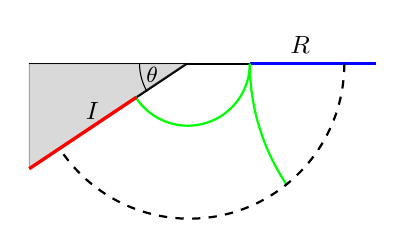
\begin{tikzpicture}[scale=0.8]
			\draw (-2.5,0) -- (0,0);
			\draw[thick](0,0) -- (1,0);
			\draw[very thick,blue] (1,0) -- (3,0);
			
			\node [anchor=south] at (1.8,0) {\small $R$};
			
			\draw[thick] (0,0) -- (-2.5,-2/3*2.5);
			
			\draw[thick,green] (1,0) arc (180:214:98pt);
			\draw[thick,green] (1,0) arc (0:-148:28pt);
			\draw[thick,dashed,black] (2.5,0) arc (0:-146:70pt);
			
			\draw [fill=gray,opacity=0.3] (0,0) -- (-2.5,0) -- (-2.5,-2/3*2.5)--(0,0);
			
			\node at (-1.5,-0.75) {\small $I$};
			\draw[very thick,red] (-0.8,-2/3*0.8) -- (-2.5,-2/3*2.5);
			
			\node at (-0.55,-0.18) {\footnotesize $\theta$};
			\draw (-0.75,0) arc (180:210:25pt);
		\end{tikzpicture}
	}
	\hskip 20mm
	\subfigure[][]{\label{fig:KR-grav}
		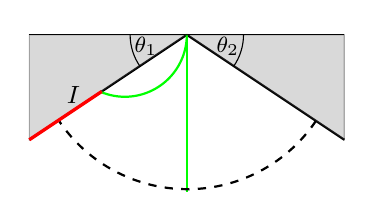
\begin{tikzpicture}[scale=0.8]
			\draw (-2.5,0) -- (2.5,0);	
			
			
			\draw[thick] (0,0) -- (-2.5,-2/3*2.5);
			\draw[thick] (0,0) -- (2.5,-2/3*2.5);
			
			\draw[thick,green] (0,0) -- (0,-2.5);
			\draw[thick,green] (0,0) arc (0:-113:28pt);
			\draw[thick,dashed,black] (2.05,-2/3*2.05) arc (-34:-146:70pt);
			
			\draw [fill=gray,opacity=0.3] (0,0) -- (-2.5,0) -- (-2.5,-2/3*2.5)--(0,0);
			\draw [fill=gray,opacity=0.3] (0,0) -- (2.5,0) -- (2.5,-2/3*2.5)--(0,0);
			
			\node at (-1.8,-0.95) {\small $I$};
			\draw[very thick,red] (-1.35,-2/3*1.35) -- (-2.5,-2/3*2.5);
			
			\node at (-0.65,-0.18) {\footnotesize $\theta_{1}$};
			\node at (0.65,-0.18) {\footnotesize $\theta_2$};
			\draw (-0.9,0) arc (180:215:25pt);
			\draw (0.9,0) arc (0:-35:25pt);
		\end{tikzpicture}
	}
	
	\caption{
		Left: Karch/Randall model for non-gravitating bath. The figure shows part of $AdS_5$ with the ETW brane cutting off the shaded region.
		The dashed curve is the black hole horizon and $R$ is the radiation region (blue). 
		The green curve ending on the horizon represents the HM surface; 
		the green curve extending from the boundary of $R$ to the ETW brane is the island surface. $I$ is the island (red).
		Right: For a gravitating bath a second ETW brane is introduced, leaving only a 3-dimensional part of the conformal boundary.
		\label{fig:KR}}
\end{figure}




A gravitating bath can be realized by introducing a second ETW brane as bath (fig.~\ref{fig:KR-grav}) \cite{Geng:2020fxl}.
This modifies description (b) to now comprise two CFTs coupled to gravity on distinct $AdS_4$ spaces, and coupled to each other at the conformal boundaries.
Description (c) is reduced to a 3d CFT.
Since both ETW branes have dynamical gravity, a conventional geometric EE can not be defined on the second ETW brane.
If one allows the end points of minimal surfaces on both ETW branes to be chosen dynamically, the surfaces can settle on the horizon and lead to a flat entropy curve, in line with the general arguments of \cite{Laddha:2020kvp}.
The quantity that was found to exhibit Page curve behavior in \cite{Geng:2020fxl} instead corresponds to minimal surfaces anchored at the remaining point of the conformal boundary of $AdS_5$, and was interpreted as EE between defect degrees of freedom represented by the left and right ETW branes.
The form of the entropy curve was found to have interesting dependence on the ETW brane angles, as will be discussed in more detail below.


\medskip
\textbf{Islands and Page curves in Type IIB:}
In this work we will study 10d  string theory versions of the Karch/Randall models
and show that the qualitative features captured by the bottom-up models are realized in a  UV-complete theory of quantum gravity.
We will discuss black holes coupled to non-gravitating and to gravitating baths, realized through 10d black hole solutions based on the $AdS_4\times S^2\times S^2\times\Sigma$ solutions of Type IIB constructed in \cite{DHoker:2007zhm,DHoker:2007hhe,Aharony:2011yc,Assel:2011xz}.



\begin{figure}
	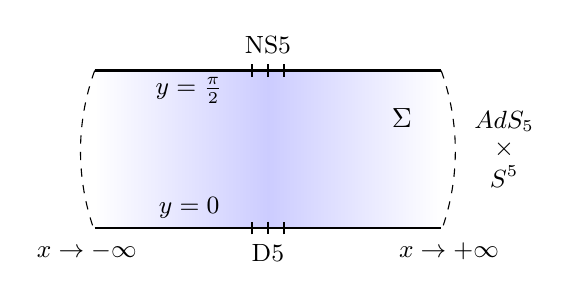
\begin{tikzpicture}
		\shade [ left color=blue! 0, right color=blue! 20] (-2.2,0)  rectangle (0,-2);
		\shade [ right color=blue! 0, left color=blue! 20] (0,0)  rectangle (2.2,-2);
		
		\draw[thick] (-2.2,0) -- (2.2,0);
		\draw[thick] (-2.2,-2) -- (2.2,-2);
		\draw[dashed] (-2.2,0) arc (160:200:85pt);
		\draw[dashed] (2.2,0) arc (20:-20:85pt);
		
		\node at (1.7,-0.6) {$\Sigma$};
		\node at (2.3,-2.3) {\small $x\rightarrow+\infty$};
		\node at (-2.3,-2.3) {\small $x\rightarrow-\infty$};
		\node at (3.0,-0.65) {\small $AdS_5$};
		\node at (3.0,-1) {\small $\times$};
		\node at (3.0,-1.35) {\small $S^5$};
		
		\draw[thick] (0.2,-0.08) -- (0.2,0.08);
		\draw[thick] (-0.2,-0.08) -- (-0.2,0.08);
		\draw[thick] (0,-0.08) -- (0,0.08) node [anchor=south] {\small NS5};
		\draw[thick] (0.2,-2-0.08) -- (0.2,-2+0.08);
		\draw[thick] (-0.2,-2-0.08) -- (-0.2,-2+0.08);
		\draw[thick] (0,-1.92) -- (0,-2.08) node [anchor=north] {\small D5};
		
		\node at (-1,-1.75) {\small $y=0$};
		\node at (-1,-0.25) {\small $y=\frac{\pi}{2}$};
		
	\end{tikzpicture}
\qquad\qquad
	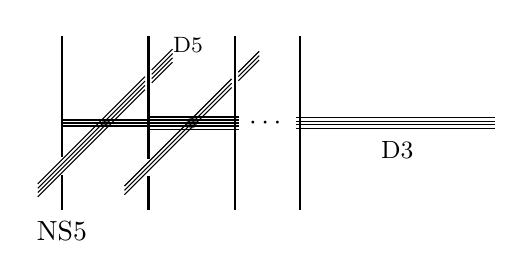
\begin{tikzpicture}[y={(0cm,1cm)}, x={(0.707cm,0.707cm)}, z={(1cm,0cm)}, scale=1.1]
	\draw[white,fill=gray!100] (0,0,0.5) circle (1.5pt);
	\draw[white,fill=gray!100] (0,0,1.5) circle (2pt);
	
	\draw[thick] (0,-0.39,0) -- (0,1,0);
	\draw[thick] (0,-1,0) -- (0,-0.6,0);
	
	\draw[thick] (0,-0.41,1) -- (0,1,1);
	\draw[thick] (0,-1,1) -- (0,-0.61,1);
	
	\draw[thick] (0,-1,2) -- (0,1,2);
	
	\node at (0,0,2.375) {$\cdots$};
	\draw[thick] (0,-1,2.75) -- (0,1,2.75);
	
	\foreach \i in {-0.075,-0.025,0.025,0.075}{ \draw (-1.1,\i,0.5) -- (0.65,\i,0.5);}
	\foreach \i in {-0.075,-0.025,0.025,0.075}{ \draw (0.76,\i,0.5) -- (1.1,\i,0.5);}
	
	\foreach \i in {-0.05,0,0.05}{ \draw (-1.1,\i,1.5) -- (0.65,\i,1.5);}
	\foreach \i in {-0.05,0,0.05}{ \draw (0.76,\i,1.5) -- (1.1,\i,1.5);}
	
	\foreach \i in {-0.025,0,0.025}{ \draw (0,1.4*\i,0) -- (0,1.4*\i,1);}
	\foreach \i in {-0.05,-0.025,0,0.025,0.05}{ \draw (0,1.4*\i,1) -- (0,1.4*\i,2.05);}
	\foreach \i in {-0.045,-0.015,0.015,0.045}{ \draw (0,1.4*\i,2.7) -- (0,1.4*\i,5);}
	
	\node at (-0.18,-0.18,4) {\small D3};
	\node at (1.0,0.2,0.75) {\footnotesize D5};
	\node at (0,-1.25) {NS5};
\end{tikzpicture}
	
\caption{
	Left: Geometry of $AdS_4\times S^2\times S^2\times\Sigma$ solutions with $\Sigma=\lbrace x+iy\in\mathds{C}\vert \,0\leq y\leq \frac{\pi}{2}\rbrace$ for non-gravitating baths. On each boundary component an $S^2$ collapses, so the 10d geometry is closed.
	D5/NS5 brane sources are located on the $y=0$/$y=\frac{\pi}{2}$ boundaries.
	The limit $x\rightarrow -\infty$ is a regular point of the internal space.
	For $x\rightarrow\infty$ the solutions approach locally $AdS_5\times S^5$; this region corresponds to the conformal boundary in fig.~\ref{fig:KR-nongrav}.
	The ETW brane in fig.~\ref{fig:KR-nongrav} can be seen as effective description for the remaining 10d geometry.
	Right: Associated configuration of D5, NS5 and D3 branes, with D3-branes suspended between 5-branes and semi-infinite D3-branes emerging in one direction. The distribution of 5-brane sources in the supergravity solution encodes how many D5/NS5 branes there are and how the D3-branes  end on them.
	\label{fig:AdS4-sol}}
\end{figure}



We start the discussion with non-gravitating baths.
The solutions constructed in \cite{DHoker:2007zhm,DHoker:2007hhe,Aharony:2011yc} can be used to describe semi-infinite D3-branes terminating on a system of D5 and NS5 branes with additional D3-branes suspended between the 5-branes.
The brane configurations engineer $\mathcal N=4$ SYM on a half space, corresponding to the semi-infinite D3-branes, coupled to a 3d SCFT on the boundary, corresponding to the D3-branes suspended between the D5 and NS5 branes. 
The structure of the supergravity solutions and brane setups is illustrated in fig.~\ref{fig:AdS4-sol}.
At each point of $\Sigma$ there is an $AdS_4$ and two 2-spheres, with independently varying radii.
%
The region $x\rightarrow\infty$ where the geometry becomes $AdS_5\times S^5$ is modeled in the Karch/Randall models in fig.~\ref{fig:KR-nongrav} by the $AdS_5$ region far away from the ETW brane.
The ETW brane itself can be understood as effective description for the remaining part of the 10d solution, i.e.\ the region around the 5-brane sources in fig.~\ref{fig:AdS4-sol}.
The intermediate holographic description, in which only the defect degrees of freedom are geometrized (description (b) above), corresponds to $AdS_4$ gravity in the region away from the $AdS_5\times S^5$ part coupled at the conformal boundary of $AdS_4$ to $\mathcal N=4$ SYM on a half space.
The 4d graviton has a mass, which, in the limit where the number of semi-infinite D3-branes is small, is set by the ratio of 4d and 3d central charges \cite{Bachas:2018zmb}.
We will modify these solutions by introducing black holes on the $AdS_4$ spaces, which leads to non-supersymmetric solutions of Type IIB that are asymptotic to the supersymmetric seed solutions and describe the dual QFTs at finite temperature.

The radiation region $R$ will be defined in the asymptotic $AdS_5\times S^5$ region at $x\rightarrow\infty$ in fig.~\ref{fig:AdS4-sol}, while the ``physical black hole'' corresponds to the region around the 5-brane sources.
The surfaces computing the entanglement entropy of the radiation region wrap both $S^2$'s and are anchored in the $AdS_5\times S^5$ region at a fixed value of the $AdS_4$ radial coordinate. 
For the non-gravitating baths we construct the HM surfaces explicitly at the time $t=0$ when their area is smallest.
The minimal surfaces can be described by specifying the $AdS_4$ radial coordinate $r$ as function of the coordinates on the Riemann surface $x$ and $y$.
The surfaces extend along the Riemann surface $\Sigma$, and either drop into the horizon in $AdS_4$ along a curve $x_h(y)$ (HM surfaces), or extend all the way to $x\rightarrow -\infty$, where they can close off smoothly before reaching the horizon in $AdS_4$ (island surfaces).

The extremality condition is a non-linear PDE on $\Sigma$. 
The boundary conditions will be derived from regularity of the induced metric on the minimal surface,
which will give a string theory justification for the use of Neumann boundary conditions at the ETW brane in the Karch/Randall models (other boundary conditions in 5d were discussed in \cite{Ghosh:2021axl}).
Solutions to the PDE are obtained numerically.
The class of $AdS_4\times S^2\times S^2\times \Sigma$ solutions is very broad, reflecting the breadth of brane configurations that can be realized with D3, D5 and NS5 branes.
We will choose representative solutions with $N_5$ D5-branes at $(x,y)=(0,0)$, $N_5$ NS5-branes at $(x,y)=(0,\frac{\pi}{2})$ and $2N_5K$ semi-infinite D3-branes. Studying more general solutions will be left for the future.

The 8d minimal surfaces can be visualized as 2d surfaces in the 3d space spanned by $\Sigma$ and the $AdS_4$ radial direction $r$,
with the horizon at some finite $r_h$. The conformal boundary of $AdS_4$ at $r\rightarrow\infty$ corresponds to the defect in fig.~\ref{fig:KR-nongrav}.
A sample of island and HM surfaces is shown in figs.~\ref{fig:islands}, \ref{fig:HM-surf}.
The island surfaces show distinct behavior near the 5-brane sources, which is discussed in sec.~\ref{sec:near-pole}.
The area differences between island surfaces and HM surfaces at $t=0$ are shown in fig.~\ref{fig:areadiff}. 
%
The results show that for radiation regions starting far in the bath (small $r$), the HM surface dominates at $t=0$.
The area of the HM surface grows in time and sets the initial growth of the entropy, but the entropy growth is bounded by the constant area of the island surface. 
This evades an information paradox and shows that the entropy follows a Page curve.


\medskip
\textbf{Critical angle:}
The analysis of  \cite{Geng:2020fxl} found a critical value for the tension/angle of the ETW brane ($\theta$ in fig.~\ref{fig:KR}), where the behavior of the island surfaces changes qualitatively.
%
The critical angle $\theta_c$ can be defined as follows:
At zero temperature, for an island surface anchored at a fixed point in the bath system, one can ask for the end point on the ETW brane as function of $\theta$. For $\theta>\theta_c$ this is a finite point.
As $\theta_c$ is approached, the end point on the ETW brane diverges towards the Poincar\'e horizon and below $\theta_c$ there are no more island minimal surfaces.

Remarkably, a similar phenomenon can be identified in 10d.
The angle $\theta$ in 5d is set by the tension of the ETW brane, which can be understood as a measure for the number of degrees of freedom represented by the ETW brane.
The relevant parameters in the 10d solutions considered here are the radius of the asymptotic $AdS_5\times S^5$ region, which is set by the number of semi-infinite D3-branes, and the number of D5 and NS5 branes on which the D3-branes terminate. 
The latter determines the 3d SCFT that $\mathcal N=4$ SYM is coupled to at the boundary of the half space.
One may expect that the brane angle in 5d captures the ratio of the number of D3-branes suspended between 5-branes and the number of semi-infinite D3-branes.
%
This is indeed the case: For island surfaces at zero temperature, with fixed anchor point in the $AdS_5\times S^5$ region, the end point at $x=-\infty$ is shown as function of $N_5/K$, which controls the ratio of suspended and semi-infinite D3-branes, in fig.~\ref{fig:crit-ang}.
The results indicate that there is a critical ratio at which the end point at $x=-\infty$ runs off towards the Poincar\'e horizon.
For black hole solutions with finite temperature this behavior is regulated (fig.~\ref{fig:crit-ang-T}), and island surfaces can be found  beyond the critical ratio.


\medskip
\textbf{Gravitating baths:} 
For the description of a gravitating bath the asymptotic $AdS_5\times S^5$ region in fig.~\ref{fig:AdS4-sol} is closed off. 
This corresponds to removing the semi-infinite D3-branes from the brane setup, leaving only D3-branes suspended between D5 and NS5 branes (fig.~\ref{fig:AdS4-sol-grav}). 
This is captured in the 5d Karch/Randall models by the introduction of a second ETW brane. 
The 10d solutions are holographic duals for 3d $T_\rho^\sigma[SU(N)]$ SCFTs \cite{Assel:2011xz} and have massless 4d gravitons.
Closing off the $AdS_5\times S^5$ region removes the part in which the radiation region was defined,
and a minimal surface stretching from $x=-\infty$ to $x=+\infty$ now has to satisfy Neumann boundary conditions on both ends. This allows it to settle onto the black hole horizon and  leads to a constant entropy identical to the thermal entropy of the bath, 
 in line with the general arguments of \cite{Laddha:2020kvp,Raju:2020smc}.

\begin{figure}
	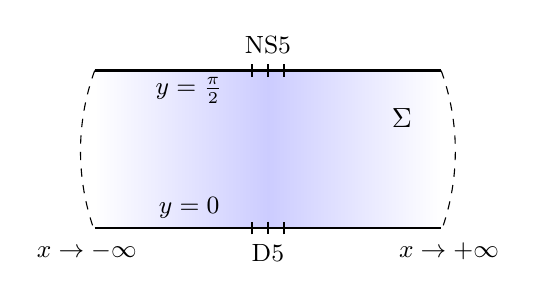
\begin{tikzpicture}
		\shade [ left color=blue! 0, right color=blue! 20] (-2.2,0)  rectangle (0,-2);
		\shade [ right color=blue! 0, left color=blue! 20] (0,0)  rectangle (2.2,-2);
		
		\draw[thick] (-2.2,0) -- (2.2,0);
		\draw[thick] (-2.2,-2) -- (2.2,-2);
		\draw[dashed] (-2.2,0) arc (160:200:85pt);
		\draw[dashed] (2.2,0) arc (20:-20:85pt);
		
		\node at (1.7,-0.6) {$\Sigma$};
		\node at (2.3,-2.3) {\small $x\rightarrow+\infty$};
		\node at (-2.3,-2.3) {\small $x\rightarrow-\infty$};
		
		\draw[thick] (0.2,-0.08) -- (0.2,0.08);
		\draw[thick] (-0.2,-0.08) -- (-0.2,0.08);
		\draw[thick] (0,-0.08) -- (0,0.08) node [anchor=south] {\small NS5};
		\draw[thick] (0.2,-2-0.08) -- (0.2,-2+0.08);
		\draw[thick] (-0.2,-2-0.08) -- (-0.2,-2+0.08);
		\draw[thick] (0,-1.92) -- (0,-2.08) node [anchor=north] {\small D5};
		
		\node at (-1,-1.75) {\small $y=0$};
		\node at (-1,-0.25) {\small $y=\frac{\pi}{2}$};
		
	\end{tikzpicture}
	\qquad\qquad
	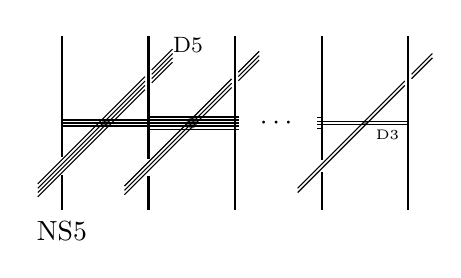
\begin{tikzpicture}[y={(0cm,1cm)}, x={(0.707cm,0.707cm)}, z={(1cm,0cm)}, scale=1.1]
		\draw[white,fill=gray!100] (0,0,0.5) circle (1.5pt);
		\draw[white,fill=gray!100] (0,0,1.5) circle (2pt);
		\draw[white,fill=gray!100] (0,0,3.5) circle (1pt);
		
		\draw[thick] (0,-0.39,0) -- (0,1,0);
		\draw[thick] (0,-1,0) -- (0,-0.6,0);
		
		\draw[thick] (0,-0.41,1) -- (0,1,1);
		\draw[thick] (0,-1,1) -- (0,-0.61,1);
		
		\draw[thick] (0,-1,2) -- (0,1,2);
		
		\node at (0,0,2.5) {$\cdots$};
		
		\draw[thick] (0,-0.43,3) -- (0,1,3);
		\draw[thick] (0,-1,3) -- (0,-0.57,3);
		
		\foreach \i in {-0.075,-0.025,0.025,0.075}{ \draw (-1.1,\i,0.5) -- (0.65,\i,0.5);}
		\foreach \i in {-0.075,-0.025,0.025,0.075}{ \draw (0.76,\i,0.5) -- (1.1,\i,0.5);}
		
		\foreach \i in {-0.05,0,0.05}{ \draw (-1.1,\i,1.5) -- (0.65,\i,1.5);}
		\foreach \i in {-0.05,0,0.05}{ \draw (0.76,\i,1.5) -- (1.1,\i,1.5);}
		
		\foreach \i in {-0.025,0.025}{ \draw (-1.1,\i,3.5) -- (0.65,\i,3.5);}
		\foreach \i in {-0.025,0.025}{ \draw (0.76,\i,3.5) -- (1.1,\i,3.5);}
		
		\foreach \i in {-0.025,0,0.025}{ \draw (0,1.4*\i,0) -- (0,1.4*\i,1);}
		\foreach \i in {-0.05,-0.025,0,0.025,0.05}{ \draw (0,1.4*\i,1) -- (0,1.4*\i,2.05);}
		\foreach \i in {-0.045,-0.015,0.015,0.045}{ \draw (0,1.4*\i,2.95) -- (0,1.4*\i,3);}
		\foreach \i in {-0.015,0.015}{ \draw (0,1.4*\i,3) -- (0,1.4*\i,4);}
		
		\draw[thick] (0,-1,4) -- (0,1,4);
		
		\node at (-0.2,0,3.9) {\tiny D3};
		\node at (1.0,0.2,0.75) {\footnotesize D5};
		\node at (0,-1.25) {NS5};
	\end{tikzpicture}
	
	\caption{
		Left: $AdS_4\,{\times}\, S^2\,{\times}\, S^2\,{\times}\,\Sigma$ solutions for gravitating baths. The $AdS_5\times S^5$ region is closed off; the limits $x\rightarrow \pm\infty$ both lead to regular points in the internal space.
		This leaves the 3d conformal boundary of $AdS_4$, corresponding to the remaining point of the conformal boundary in fig.~\ref{fig:KR-grav}.
		Right: The associated brane configurations have no semi-infinite D3-branes, only D3-branes suspended between 5-branes.
		\label{fig:AdS4-sol-grav}}
\end{figure}

One can instead consider minimal surfaces splitting the internal space, which are expected to compute non-geometric entanglement entropies (whose holographic interpretation was initiated in \cite{Mollabashi:2014qfa,Karch:2014pma}).
%
In the Karch/Randall models a ``left/right EE", represented by surfaces ending on the point where the two ETW branes meet in fig.~\ref{fig:KR-grav}, was found to exhibit Page curve behavior, and was interpreted as an internal entanglement entropy in \cite{Geng:2020fxl}.
%
The Type IIB solutions realize the dual of the defect as full 10d geometry, making them an ideal setting for studies of minimal surfaces separating degrees of freedom according to their representation in the internal space.

We consider surfaces wrapping the spatial part of $AdS_4$, both $S^2$'s, and a curve in $\Sigma$ which depends on the $AdS_4$ radial coordinate.
The surfaces are anchored at the conformal boundary of $AdS_4$ along a curve $x(y)$ in $\Sigma$ which separates the 5-brane sources and defines a split into black hole system and bath. 
Such surfaces may be expected to compute EEs associated with decompositions of the quiver diagram in the UV description of the dual 3d SCFT.
One again has to consider HM surfaces, extending through the horizon in $AdS_4$ into the thermofield double, and island surfaces which close off in one of the $x\rightarrow\pm\infty$ regions before reaching the horizon in $AdS_4$. These are 10d versions of the surfaces in fig.~\ref{fig:KR-grav}.
%
The class of $AdS_4\times S^2\times S^2\times \Sigma$ solutions that could be considered is again broad, and we focus on simple representatives.
We include two groups of D5-branes and two groups of NS5 branes, placed symmetrically at $x=\pm \delta$ on the boundary components of $\Sigma$. 
%
The separation of the 5-brane sources determines how the D3-branes in the associated brane configuration are suspended between the 5-branes.
Comparing to the Karch/Randall models in fig.~\ref{fig:KR-grav}, these particular 10d solutions correspond to two equal ETW brane angles.

Some 10d island surfaces are shown in fig.~\ref{fig:LRcrit2}. 
The corresponding HM surface is described by $x=0$ and a time-dependent embedding in the $AdS_4$ part of the geometry.
The difference in areas between island and HM surfaces at $t=0$ is shown in fig.~\ref{fig:LRcrit1b}.
We find that for $\delta$ above a ``Page value" $\delta_P$ the HM surface initially dominates at $t=0$.
The entropy growth indicated by the HM surfaces is bounded by the constant area of the island surfaces, leading again to Page curves, shown in fig.~\ref{fig:page}.
A second distinguished value for $\delta$ can be seen in fig.~\ref{fig:LRcrit1a}:
at a critical value $\delta_c$ the cap-off point of the island surface at $x=-\infty$ diverges towards the conformal boundary of $AdS_4$,
and no island minimal surfaces are found for $\delta<\delta_c$.
The numerical results suggest that $\delta_c$ is slightly smaller than $\delta_P$, though we leave the possibility that the difference could be a numerical artifact.
In the small (and possibly empty) range $\delta_c<\delta<\delta_P$ the island surfaces are found to dominate already at $t=0$, leading to a flat entropy curve.
These results bear striking resemblance with critical and Page angles found in the Karch/Randall models in \cite{Geng:2020fxl}, suggesting that the ETW brane angles capture aspects of how the 5-brane sources are distributed on $\Sigma$ in~10d.

In the regime where no island minimal surfaces were found in the 5d Karch/Randall models in \cite{Geng:2020fxl}, ``tiny island"
limiting surfaces, which degenerate to an infinitesimal segment at the defect in fig.~\ref{fig:KR-grav}, were found to dominate and limit the entropy growth indicated by the HM surface.
%
In 10d we find that similar tiny island surfaces connecting the $x=0$ locus to $x=\pm\infty$ arise for $\delta<\delta_c$.


\medskip 
\textbf{Outline:} 
The main part is organized as follows.
The 10d supergravity solutions are introduced in sec.~\ref{sec:IIBsol}.
In sec.~\ref{sec:surfaces} the ansatz for extremal surfaces is discussed along with the extremality and boundary conditions and the behavior near the 5-branes.
The method for constructing minimal surfaces is summarized in sec.~\ref{sec:numerics}.
%
Island surfaces and Page curves are discussed for non-gravitating baths  in sec.~\ref{sec:islands} and for gravitating baths in sec.~\ref{sec:grav-bath}. We close with a brief outlook in sec.~\ref{sec:outlook}.



\section{Type IIB supergravity solutions}\label{sec:IIBsol}

The general local form of the $AdS_4\times S^2\times S^2\times \Sigma$ solutions that will be used here was constructed in \cite{DHoker:2007zhm,DHoker:2007hhe}. 
For the study of minimal surfaces we will only need the geometry, which is a warped product of $AdS_4$ and two 2-spheres, $S_1^2$ and $S_2^2$, over a Riemann surface $\Sigma$.
For the solutions of interest here $\Sigma$ can be taken as a strip, 
\begin{align}
	\Sigma&=\lbrace z\in\mathds{C}\,\vert\, 0\leq \Im(z)\leq \pi/2\rbrace~.
\end{align}
On each of the boundary components of the strip one of the $S^2$'s closes off smoothly, so that the 10d geometry has no boundary.
Depending on the nature of the points at infinity, solutions for different types of field theories can be constructed: 
Janus solutions, dual to interface CFTs, can be realized if the points $\Re(z)\rightarrow \pm\infty$ both correspond to asymptotic $AdS_5\times S^5$ regions.
Solutions with one asymptotic region closed off were constructed in \cite{Aharony:2011yc} and are dual to BCFTs.
Duals for 3d SCFTs were constructed in \cite{Assel:2011xz} by closing both asymptotic $AdS_5\times S^5$ regions.

The solutions are generally parametrized by two harmonic functions $h_1$, $h_2$ on $\Sigma$.
The Einstein-frame metric takes the form
\begin{align}\label{eq:10d-metric}
	ds^2&=f_4^2 ds^2_{4}+f_1^2 ds^2_{S_1^2}+f_2^2 ds^2_{S_2^2}+4\rho^2 |dz|^2~,
\end{align}
where $ds^2_{4}$ and $ds^2_{S_i^2}$ are line elements of unit-radius $AdS_4$ and $S^2$, respectively.
The coefficient functions are given by
\begin{align}
	f_4^8&=16\frac{N_1N_2}{W^2}~, & f_1^8&=16h_1^8\frac{N_2 W^2}{N_1^3}~, & f_2^8&=16 h_2^8 \frac{N_1 W^2}{N_2^3}~,
	&
	\rho^8&=\frac{N_1N_2W^2}{h_1^4h_2^4}~,
\end{align}
where
\begin{align}
	W&=\partial\bar\partial (h_1 h_2)~, & N_i &=2h_1 h_2 |\partial h_i|^2 -h_i^2 W~.
\end{align}
The expressions for the fluxes and dilaton will not be needed here; they can be found in \cite{DHoker:2007zhm,DHoker:2007hhe,Aharony:2011yc,Assel:2011xz}.

Based on this local form broad classes of supergravity solutions can be constructed which describe D3-branes intersecting, ending on, or suspended between D5 and NS5 branes.
For the realization of Karch/Randall models with gravitating and non-gravitating baths we will employ representative solutions dual to BCFTs and 3d SCFTs, noting that more general solutions could be considered.
The form of the harmonic functions $h_1$, $h_2$ is
\begin{align}
	h_1&=\frac{\pi \alpha^\prime}{4} K e^z-\frac{\alpha^\prime}{4} \sum_{a}N_{\rm D5}^{(a)}\ln\tanh\left(\frac{z-\delta_a}{2}\right)+\rm{c.c.}
	\nonumber\\
	h_2&=-\frac{i \pi \alpha^\prime}{4} K e^z-\frac{\alpha^\prime}{4}\sum_b N_{\rm NS5}^{(b)}\ln\tanh\left(\frac{i\pi}{4}-\frac{z-\delta_b}{2}\right)+\rm{c.c.}
\end{align}
The solutions describe semi-infinite D3-branes ending on D5-branes and NS5-branes which have additional D3-branes suspended between them.
The number of semi-infinite D3-branes is controlled by $K$; for $K=0$ the solutions describe D3-branes suspended between D5 and NS5 branes.
Groups of D5/NS5 branes are represented by the poles of $\partial h_1$/$\partial h_2$ on the boundary of $\Sigma$.
The specific brane configuration can be characterized in terms of linking numbers, which are encoded in the distribution of the 5-brane sources on $\Sigma$ \cite{Aharony:2011yc,Assel:2011xz}.
For $K\neq 0$ an $AdS_5\times S^5$ region emerges at $\Re(z)\rightarrow + \infty$, with $\Re(z)$ becoming the radial coordinate of $AdS_5$ in $AdS_4$ slicing and $\Im(z)$ becoming an angular coordinate on $S^5$.
For $K=0$ the limit $\Re(z)\rightarrow\infty$ leads to a regular point in the internal space.
The limit $\Re(z)\rightarrow -\infty$ leads to a regular point in both cases.


We discuss the concrete solutions that will be used below first and briefly comment on the more general picture and dual field theories afterwards.
The solutions we will study for non-gravitating baths are dual to $\mathcal N=4$ SYM on a half space coupled to 3d $T_\rho^\sigma[SU(N)]$ theories on the boundary.
They are given by $h_{1/2}$ of the form
\begin{align}\label{eq:h1h2-BCFT}
	h_1&=\frac{\pi \alpha^\prime}{4} K e^z-\frac{\alpha^\prime}{4}N_5\ln\tanh\left(\frac{z}{2}\right)+\rm{c.c.}
	\nonumber\\
	h_2&=-\frac{i\pi\alpha^\prime}{4}K e^z-\frac{\alpha^\prime}{4}N_5\ln\tanh\left(\frac{i\pi}{4}-\frac{z}{2}\right)+\rm{c.c.}
\end{align}
The radii of $AdS_5$ and $S^5$ in the $AdS_5\times S^5$ region at $\Re(z)\rightarrow\infty$ are set by $L^4=8\pi{\alpha^\prime}^2N_5K$.
The asymptotic string coupling is $\lim_{x\rightarrow\infty}e^\phi=1$.
These solutions are string theory realizations of the Karch/Randall models with one ETW brane (fig.~\ref{fig:KR-nongrav}): the asymptotic region at $\Re(z)\rightarrow\infty$ corresponds to the $AdS_5$ part, while the region with the NS5/D5 sources is the string theory version of the ETW brane itself.
%
The brane configuration involves $2N_5K$ semi-infinite D3-branes ending on a combination of $N_5$ D5-branes and $N_5$ NS5-branes (fig.~\ref{fig:brane-non-grav}).
$N_5K$ D3-branes end on the D5 branes and $N_5K$ D3-branes end on the NS5-branes, and there are in addition $N_5^2/2$ D3-branes suspended between the D5 and NS5 branes.


\begin{figure}
	\subfigure[][]{\label{fig:brane-non-grav}
	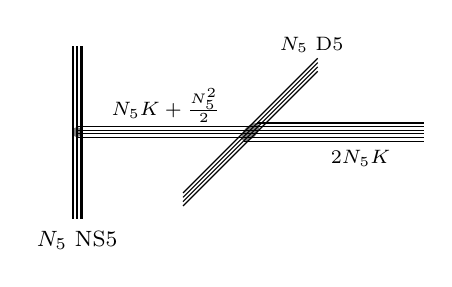
\begin{tikzpicture}[y={(0cm,1cm)}, x={(0.707cm,0.707cm)}, z={(1cm,0cm)}, scale=1.1]
	\draw[gray,fill=gray!100,rotate around={-45:(0,0,2)}] (0,0,2) ellipse (1.8pt and 3.5pt);
	\draw[gray,fill=gray!100] (0,0,0) circle (1.5pt);
	
	\foreach \i in {-0.05,0,0.05}{ \draw[thick] (0,-1,\i) -- (0,1,\i);}
	
	
	\foreach \i in {-0.075,-0.025,0.025,0.075}{ \draw (-1.1,\i,2) -- (1.1,\i,2);}
		
	\foreach \i in {-0.045,-0.015,0.015,0.045}{ \draw (0,1.4*\i,0) -- (0,1.4*\i,2+\i);}
	\foreach \i in  {-0.075,-0.045,-0.015,0.015,0.045,0.075}{ \draw (0,1.4*\i,2+\i) -- (0,1.4*\i,4);}
	
	\node at (-0.18,-0.18,3.4) {\scriptsize $2N_5 K$};
	\node at (1.0,0.3,2) {\scriptsize $N_5$ D5};
	\node at (0,-1.25) {\footnotesize $N_5$ NS5};
	\node at (0.18,0.18,0.9) {{\scriptsize $N_5 K+\tfrac{N_5^2}{2}$}};
\end{tikzpicture}
}
\hskip 20mm
\subfigure[][]{\label{fig:brane-grav}
		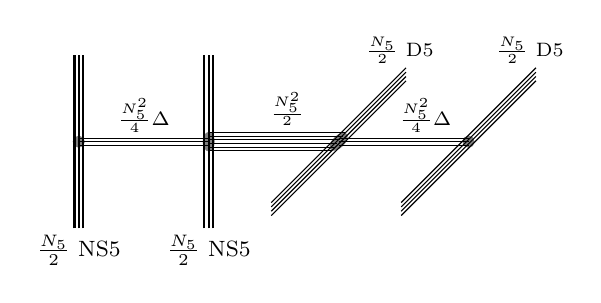
\begin{tikzpicture}[y={(0cm,1cm)}, x={(0.707cm,0.707cm)}, z={(1cm,0cm)}, scale=1.1]
		\draw[gray,fill=gray!100] (0,0,-0.5) circle (1.8pt);
		\draw[gray,fill=gray!100] (0,0,1) ellipse (1.8pt and 3pt);
		\draw[gray,fill=gray!100,rotate around={-45:(0,0,2.5)}] (0,0,2.5) ellipse (1.8pt and 3.5pt);
		\draw[gray,fill=gray!100] (0,0,4) circle (1.8pt);				
		
		\foreach \i in {-0.05,0,0.05}{ \draw[thick] (0,-1,-0.5+\i) -- (0,1,-0.5+\i);}
		\foreach \i in {-0.05,0,0.05}{ \draw[thick] (0,-1,1+\i) -- (0,1,1+\i);}


		\foreach \i in {-0.075,-0.025,0.025,0.075}{ \draw (-1.1,\i,2.5) -- (1.1,\i,2.5);}
		\foreach \i in {-0.075,-0.025,0.025,0.075}{ \draw (-1.1,\i,4) -- (1.1,\i,4);}
		
		\foreach \i in {-0.03,0,0.03}{ \draw (0,1.4*\i,-0.5) -- (0,1.4*\i,1);}
		\foreach \i in {-0.075,-0.045,-0.015,0.015,0.045,0.075}{ \draw (0,1.4*\i,1) -- (0,1.4*\i,2.5+\i);}
		\foreach \i in {-0.03,0,0.03}{ \draw (0,1.4*\i,2.5) -- (0,1.4*\i,4);}

		\node at (0,-1.25,-0.5) {\footnotesize $\tfrac{N_5}{2}$ NS5};
		\node at (0,-1.25,1) {\footnotesize $\tfrac{N_5}{2}$ NS5};
		\node at (1.0,0.35,2.5) {\scriptsize  $\tfrac{N_5}{2}$ D5};
		\node at (1.0,0.35,4) {\scriptsize  $\tfrac{N_5}{2}$ D5};
		\node at (0.22,0.22,1.75) {{\scriptsize $\tfrac{N_5^2}{2}$}};
		\node at (0,0.3,0.25) {{\scriptsize $\tfrac{N_5^2}{4}\Delta$}};
		\node at (0,0.3,3.5) {{\scriptsize $\tfrac{N_5^2}{4}\Delta$}};
	\end{tikzpicture}
}
\caption{Brane configurations for representative non-gravitating bath solutions (left) and gravitating bath solutions (right). 
	Hanany-Witten transitions can be used to make the 3d quiver gauge theories more apparent, as in figs.~\ref{fig:AdS4-sol}, \ref{fig:AdS4-sol-grav}. The numbers of D3-branes  on the right are controlled by $\delta$ through $\Delta=\frac{1}{2}+\frac{2}{\pi}\arctan e^{2\delta}$.
}
\end{figure}






The solutions for gravitating baths that will be considered below are holographic duals for 3d $T_\rho^\sigma[SU(N)]$ SCFTs.
The functions $h_1$ and $h_2$ are given by
\begin{align}\label{eq:h1h2-3d-grav}
	h_1&=-\frac{\alpha^\prime}{4}\frac{N_5}{2}\left[\ln\tanh\left(\frac{z-\delta}{2}\right)+
\ln	\tanh\left(\frac{z+\delta}{2}\right)\right]+\rm{c.c.}
	\nonumber\\
	h_2&=-\frac{\alpha^\prime}{4}\frac{N_5}{2}\left[\ln\tanh\left(\frac{i\pi}{4}-\frac{z-\delta}{2}\right)
	+\ln\tanh\left(\frac{i\pi}{4}-\frac{z+\delta}{2}\right)\right]+\rm{c.c.}
\end{align}
These solutions describe $N_5^2/2$ D3-branes suspended between two groups of D5-branes and two groups of NS5-branes, with $N_5/2$ 5-branes in each group.
There are no semi-infinite D3-branes and the asymptotic $AdS_5\times S^5$ region at $\Re(z)\rightarrow \infty$ is closed off.
The limits $\Re(z)\rightarrow \pm\infty$ both correspond to regular points in the internal space.
%
The 5-brane groups are represented in the supergravity solutions by sources with $N_5/2$ D5 and $N_5/2$ NS5-branes, respectively, at $z=\pm\delta$ and $z=\pm\delta+i\pi/2$. The parameter $ \delta$ determines how the D3-branes terminate on the D5 and NS5 branes (fig.~\ref{fig:brane-grav}); for $\delta=0$ the numbers of D3-branes terminating on each group of 5-branes are equal.
The dual 3d SCFTs are special cases of the theories discussed in sec.~5.3 of \cite{Coccia:2020wtk}.
%
Comparing to the 5d Karch/Randall models, the closing off of the asymptotic $AdS_5\times S^5$ region corresponds to the introduction of the second ETW brane in fig.~\ref{fig:KR-grav}. The entire 10d solution corresponds to the remaining wedge of $AdS_5$ in fig.~\ref{fig:KR-grav}.

The solutions (\ref{eq:h1h2-BCFT}) and (\ref{eq:h1h2-3d-grav}) are invariant under S-duality (exchange of $h_1$ and $h_2$ combined with $z\rightarrow \frac{i\pi}{2}-z$),
reflecting that the associated brane configurations are invariant under S-duality (in fig.~\ref{fig:brane-non-grav} up to Hanany-Witten transitions).
This will be useful below. 
From now on we set $\alpha^\prime=1$.

Solutions with more general arrangements of 5-brane sources (poles in $\partial h_{1/2}$) and no asymptotic $AdS_5\times S^5$ region describe configurations of D3-branes suspended between D5 and NS5 branes that can be characterized by two Young tableaux $\rho$ and $\sigma$, which determine how precisely the D3-branes terminate on the 5-branes.
The general relation between the distribution of the 5-brane sources on the boundary of $\Sigma$ and the Young tableaux $\rho$ and $\sigma$ can be found in  \cite{Assel:2011xz}.
The brane configurations engineer 3d $\mathcal N=4$ quiver gauge theories, and the supergravity solutions are dual to their IR fixed points.
%
%
For solutions with $AdS_5\times S^5$ region and semi-infinite D3-branes the dual field theory is $\mathcal N=4$ SYM on a half space coupled to a 3d $T_\rho^\sigma[SU(N)]$ SCFT on the boundary \cite{Aharony:2011yc}. 
The free energies obtained holographically were matched to field theory computations using supersymmetric localization for the former in \cite{Assel:2012cp}, \cite{Coccia:2020wtk} and for the latter in \cite{,VanRaamsdonk:2020djx}. 


\subsection{Finite temperature}
For each  $AdS_4\times S^2\times S^2\times\Sigma$ solution one may replace $AdS_4$ by a finite temperature black hole and still obtain a solution to the Type IIB supergravity field equations:
To verify the field equations one only needs that the 4d space is Einstein with negative curvature.
This is true for the $AdS_4$ black hole metrics we will use, so that replacing $AdS_4$ by a black hole yields non-supersymmetric solutions which  asymptotically approach the supersymmetric seed solution.
From a more general perspective, the $AdS_4\times S^2\times S^2\times\Sigma$ solutions are in the class for which \cite{Gauntlett:2007ma} conjecture that a  consistent truncation exists. 
Having a consistent truncation to 4d gauged supergravity would allow to uplift more general 4d solutions to 10d, but this is not needed for our purposes here.

To introduce finite temperature, we replace the $AdS_4$ metric in (\ref{eq:10d-metric}) by 
the $AdS_4$ black hole metric
\begin{align}\label{eq:ds2-AdS4-T}
	ds_4^2&=\frac{dr^2}{b(r)}+e^{2r}\left(-b(r)dt^2+ds^2_{\RR^2}\right)~,
	&
	b(r)&=1-e^{3(r_h-r)}~.
\end{align}
The horizon is at $r=r_h$, the conformal boundary at $r\rightarrow\infty$.
It will be convenient to also introduce the tortoise coordinate $u$ by
\begin{align}\label{eq:tortoise}
	du&=\frac{dr}{\sqrt{b(r)}}~, & u&=\frac{2}{3}\cosh^{-1}\left(e^{\frac{3}{2}(r-r_h)}\right)~.
\end{align}
The range $u\in\RR^+$ corresponds to the exterior region covered by the original coordinate $r$, with the horizon at $u=0$. The metric becomes
\begin{align}
	ds^2_4&=du^2+e^{2r_h}\cosh^{4/3}\left(\frac{3u}{2}\right)\left[-\tanh^2\left(\frac{3u}{2}\right)dt^2+ds^2_{\RR^2}\right]~.
\end{align}
From the CFT perspective replacing $AdS_4$ by a planar black hole corresponds to adding a finite temperature for $\mathcal N=4$ SYM on $AdS_4$ for solutions with an $AdS_5\times S^5$ region.
The black hole solutions without $AdS_5\times S^5$ region are dual to 3d $T_\rho^\sigma[SU(N)]$ SCFTs at finite temperature.



\section{Extremal surfaces}\label{sec:surfaces}

In this section we discuss the embedding ansatz for the surfaces that will be used for the entanglement entropy computations,
the extremality and boundary conditions, and the behavior near the 5-brane sources.


\subsection{Island surfaces}

The surfaces of interest are 8d minimal surfaces in the 10d geometry (\ref{eq:10d-metric}) that wrap both $S^2$'s, (part of) the Riemann surface $\Sigma$, and a part of the $AdS_4$ black hole geometry.
For the $AdS_4$ black hole we choose coordinates (\ref{eq:ds2-AdS4-T}), such that the 10d metric is given by (\ref{eq:10d-metric}) with
\begin{align}
		ds_4^2&=\frac{dr^2}{b(r)}+e^{2r}\left(-b(r)dt^2+ds^2_{\RR^2}\right)~.
\end{align}
The surfaces can be described by specifying the $AdS_4$ radial coordinate $r$ for any given point of $\Sigma$.
On $\Sigma$ we introduce real coordinates
\begin{align}
	z=x+iy~,
\end{align}
with $x\in\mathds{R}$ and $0\leq y\leq\frac{\pi}{2}$.
The embeddings are thus described by a single embedding function
\begin{align}
	r=r(x,y)~.
\end{align}
The induced metric on the surface reads
\begin{align}\label{eq:ind-met}
	ds^2_\gamma&=e^{2r}f_4^2ds^2_{\RR^2}+f_1^2ds^2_{S_1^2}+f_2^2ds^2_{S^2_2}+4\rho^2 (dx^2+dy^2)
	+\frac{f_4^2}{b(r)}\left(dx\, \partial_x r +dy \partial_y r \right)^2~.
\end{align}
The area of a general surface of this form is given by $A=V_{\RR^2}V_{S_1^2\times S_2^2}S_\gamma$, with
\begin{align}
	S_\gamma&=4\int dx dy \,e^{2r}f_4^2f_1^2f_2^2\rho^2\sqrt{1+\frac{f_4^2}{4b(r)\rho^2}\left((\partial_x r)^2+(\partial_y r)^2\right)}~.
\end{align}
The combinations of metric functions appearing in this expression are given by
\begin{align}\label{eq:fg-eval}
	f_4^2 f_1^2f_2^2\rho^2&=8\left|h_1 h_2 W\right|~,
	&
	\frac{f_4^2}{\rho^2}&=2\left|\frac{h_1h_2}{W}\right|~.
\end{align}
With these expressions the area simplifies to
\begin{align}\label{eq:S}
	S_\gamma&=32\int dx dy \,e^{2r}\left|h_1 h_2 W\right|\sqrt{1+\frac{1}{2b(r)}\left|\frac{h_1 h_2}{W}\right| (\nabla r)^2}~.
\end{align}
Since $4W=\Delta(h_1h_2)$, the area depends on $h_1$ and $h_2$ only through the combination $h_1h_2$.


The extremality condition resulting from variation of $S_\gamma$ (with $S_\gamma=\int L_\gamma$) can be written as
\begin{align}\label{eq:eom-fg}
	0\stackrel{!}{=}	\frac{\delta L_\gamma}{L_\gamma}&=
	\frac{1}{1+g(\nabla r)^2}\left[2-\nabla(g\nabla r)+\frac{1}{2}g\nabla r\cdot \nabla\ln\left(\frac{1+g(\nabla r)^2)}{b(r) f^2}\right)\right]~,
\end{align}
where $\nabla$ is the covariant derivative with respect to the metric on $\Sigma$ and
\begin{align}
	f&=|h_1 h_2 W|~, & g&=\frac{1}{2b(r)}\left|\frac{h_1 h_2}{W}\right|~.
\end{align}
The dependence on $r$ itself drops out for zero temperature, i.e.\ when $b(r)=1$.
If $r(x,y)$ is a solution to the extremality condition at zero temperature then so is $r(x,y)+c$ with a constant $c$, with different asymptotic values at $x\rightarrow \pm\infty$; this reflects the defect conformal symmetry.


\subsection{Boundary conditions}\label{sec:bc}

We now discuss the boundary conditions for surfaces extending along $\Sigma$, starting with the two boundary components of the strip at $y=0$ and $y=\frac{\pi}{2}$.
Near $y=0$ the sphere $S_1^2$, collapses, with $f_1^2\sim 4y^2 \rho^2$ so that the background has no conical singularity in the space parametrized by $y$ and $S_1^2$.
The induced metric (\ref{eq:ind-met}) near $y=0$ consequently takes the form
\begin{align}
	ds^2_\gamma&\approx e^{2r}f_4^2ds^2_{\RR^2}+f_2^2ds^2_{S^2_2}+4\rho^2 \left( dx^2+dy^2+y^2ds^2_{S_1^2}\right)+\frac{f_4^2}{b(r)}\left(dx\, \partial_x r +dy \partial_y r \right)^2~.
\end{align}
The contribution proportional to $(\partial_y r)^2 dy^2$ threatens to introduce a conical singularity in the $(y,S_1^2)$ part of the induced metric on the surface. A smooth metric is obtained with the Neumann boundary condition $\partial_y r\vert_{y=0}=0$.
The reasoning for the second boundary component, where $S_2^2$ collapses, is analogous. We conclude
\begin{align}\label{eq:Neumann-bc-y}
	\partial_y r(x,y)\big\vert_{y=0}&=0~, & \partial_y r(x,y)\big\vert_{y=\frac{\pi}{2}}&=0~.
\end{align}

For $x\rightarrow -\infty$ the space closes off smoothly; the limit corresponds to a single regular point on the boundary of $\Sigma$. For the surface to be smooth,  $\lim_{x\rightarrow -\infty}r(x,y)$ should be independent of $y$.
The asymptotic behavior of the metric functions, with coordinate $v=2e^{x}$ and $v\rightarrow 0$, is given by (see (3.15) of \cite{Assel:2011xz})
\begin{align}
	f_4^2&\approx L^2~, & f_1^2&\approx 4\sin^2\!y\,\rho^2~, & f_2^2&\approx 4\cos^2\!y\,\rho^2~, & 4\rho^2&\approx L^2v^2~.
\end{align}
The induced metric on the minimal surface becomes (noting that $\partial_y r\rightarrow 0$)
\begin{align}
	ds^2_\gamma&\approx L^2\left[ e^{2r}ds^2_{\RR^2}+dv^2+v^2\left(dy^2+\sin^2\!y\, ds^2_{S_1^2}+\cos^2\!y\,ds^2_{S_2^2}\right)+(\partial_x r)^2\frac{dv^2}{v^2}\right]~.
\end{align}
The part in the round bracket is the line element for $S^5$, and a smooth $\RR^8$ with no conical singularity is obtained if
\begin{align}\label{eq:bc-x-minus}
	\lim_{x\rightarrow-\infty}e^{-x}\partial_x r(x,y)=0~.
\end{align}
The conditions (\ref{eq:Neumann-bc-y}) and (\ref{eq:bc-x-minus}) are the 10d analog of the Neumann boundary conditions imposed at the ETW brane in the 5d Karch/Randall models.

The nature of the limit $x\rightarrow +\infty$ is different for the solutions in (\ref{eq:h1h2-BCFT}) for a non-gravitating bath, where an $AdS_5\times S^5$ region emerges in this limit, compared to the solution (\ref{eq:h1h2-3d-grav}) for a gravitating bath.
For the latter the limits $x\rightarrow \pm \infty$ both lead to regular boundary points, and the boundary condition at $x\rightarrow+\infty$ is given by (\ref{eq:bc-x-minus}) with $x\rightarrow -x$.
For the former, with the emerging $AdS_5\times S^5$ region, a Dirichlet condition anchoring the surface is imposed instead. 
The general form is 
\begin{align}
	\lim_{x\rightarrow+\infty} r(x,y)&=r_0(y)~.
\end{align}
The form of $r_0(y)$ can be determined by considering global $AdS_5\times S^5$, corresponding to $h_1=\cosh z+\rm{c.c.}$ and $h_2=-i \sinh z+\rm{c.c.}$ 
In that case $|h_1h_2/W|=2\cosh^2(x)$, which is independent of $y$.
As a result one can find extremal surfaces with no dependence on $y$, which is an angular coordinate on $S^5$.
For more general solutions the  boundary condition in the asymptotic $AdS_5\times S^5$ region at $x\rightarrow\infty$ therefore is that $r(x,y)$ should become independent of $y$ and satisfy a Dirichlet condition with $r_0(y)=r_R$. In summary,
\begin{align}\label{eq:Dirichlet}
	\lim_{x\rightarrow+\infty}r(x,y)&=r^{}_R\qquad \text{for (\ref{eq:h1h2-BCFT}),}
	&
	\lim_{x\rightarrow+\infty}e^{+x}\partial_x r(x,y)&=0 \qquad \text{for (\ref{eq:h1h2-3d-grav}).}
\end{align}


\subsection{Near-pole behavior}\label{sec:near-pole}

At zero temperature the minimal surfaces will show distinct behavior near the 5-brane sources, and cap off there.\footnote{This differs from the behavior of the spherical entangling surface centered on the defect studied in \cite{VanRaamsdonk:2020djx}, which has a simple universal embedding which is insensitive to the 5-brane sources.}
In this section we will discuss this behavior analytically, using the form of the supergravity solutions near the 5-brane sources.
At finite temperature the behavior near the 5-brane sources will be regulated by the horizon.

To discuss the behavior near a pole at $z=z_0$ it is convenient to introduce coordinates centered on the pole, 
$z=z_0+R e^{i\varphi}$ for $z_0$ on the real line and $z=z_0-Re^{i\varphi}$ for $\Im(z_0)=\pi/2$.
The combinations that appear in the area functional (\ref{eq:S}) behave at zero temperature as follows,
\begin{align}
	f=|h_1h_2 W|&\approx f_0\sin^2(\varphi)(-\ln R)~,
	&
	g=\frac{1}{2}\left|\frac{h_1h_2}{W}\right|&\approx -R^2\ln R~,
\end{align}
where $f_0$ is a constant which depends on the solution under consideration. 
The value of $f_0$ will not be relevant, since the extremality condition (\ref{eq:eom-fg}) is invariant under constant rescalings of $f$.


To discuss the near-pole behavior it is convenient to drop the overall factor in the extremality condition (\ref{eq:eom-fg}) and use the condition in the form
\begin{align}\label{eq:eom-nb}
	0&=2-\nabla\left(g\nabla r\right)+\frac{1}{2}g\nabla r\cdot \nabla\ln\left(\frac{1+g(\nabla r)^2}{f^2}\right)~.
\end{align}
The two non-trivial terms on the right hand side are generically of the same order, noting that $\nabla \ln(\ldots)=\mathcal O(1/R)$.
A scaling analysis suggests to take $\nabla r=\mathcal O(1/(R\ln R))$ and make an ansatz
\begin{align}
	r(R,\varphi)&= r_0\ln(-\ln R)+\frac{r_1(\varphi)}{\ln R}+\ldots
\end{align}
where the ellipsis denotes regular and subleading terms.
The leading non-trivial order in the extremality condition (\ref{eq:eom-nb}) then is its finite part. 
The near-pole solution without divergences in $\varphi$ is given by $r_0=-1$ and $r_1$ constant.
In summary, the behavior of the embedding near a 5-brane source at $z=z_0$ is given by
\begin{align}\label{eq:r-near-pole}
	r(z,\bar z)&= -\ln(-\ln |z-z_0|)+\ldots~.
\end{align}
Since $\lim_{z\rightarrow z_0}r(z,\bar z)=-\infty$, the minimal surface drops into the Poincar\'e horizon at the source.
At the point $z_0$ the background geometry is singular, as appropriate for a solution near a 5-brane source, and we do not impose additional regularity conditions for the minimal surface.


\subsection{HM surfaces}

We will focus on the non-gravitating bath solutions (\ref{eq:h1h2-BCFT}) for the discussion of HM surfaces; those for the gravitating bath solutions will be discussed in sec.~\ref{sec:grav-bath}.
%
We use the tortoise coordinate $u$ defined in (\ref{eq:tortoise}) and parametrize the embedding at $t=0$ in terms of $x(u,y)$ instead of $r(x,y)$.
The minimal surfaces range in $u$ from the value enforced by the Dirichlet boundary condition (\ref{eq:Dirichlet}) through the horizon into the thermofield double.
We focus on surfaces anchored at the same point $r_R$ in the thermofield double, which are symmetric with respect to reflection across $u=0$ at $t=0$.
So we can restrict to $u\geq 0$ to find the embeddings.
From that perspective the HM surfaces end on the horizon at $u=0$ along a curve $x_h(y)$ which is determined by the extremality condition.

The induced metric with the tortoise coordinate $u$ and the parametrization $x(u,y)$ becomes 
\begin{align}
	ds^2=\,&e^{2r_h}\cosh^{4/3}\left(\frac{3u}{2}\right)f_4^2ds^2_{\mathds{R}^2}+f_1^2 ds^2_{S_1^2}+f_2^2ds^2_{S_2^2}+
	\left[f_4^2+4\rho^2(\partial_u x)^2\right]du^2
	\nonumber\\ &
	+4\rho^2 \left[dy^2\left(1+(\partial_y x)^2\right)+(\partial_u x)(\partial_y x)(du\, dy+dy\,du)\right]~.
\end{align}
The area evaluated using (\ref{eq:fg-eval}) becomes
\begin{align}\label{eq:HM-area}
	S&=32\int du dy\, e^{2r_h}\cosh^{4/3}\left(\frac{3u}{2}\right)|h_1 h_2W|\sqrt{\frac{1}{2}\left|\frac{h_1 h_2}{W}\right|\left(1+(\partial_y x)^2\right)+(\partial_u x)^2}~.
\end{align}


For the boundary conditions we start with the boundaries of $\Sigma$ at $y=0$ and $y=\frac{\pi}{2}$.
Having no conical singularities at $y=0,\frac{\pi}{2}$ leads to the Neumann boundary conditions
\begin{align}\label{eq:Neumann-bc-y-HM}
	\partial_y x(u,y)\big\vert_{y=0}&=0~, &\partial_y x(u,y)\big\vert_{y=\frac{\pi}{2}}&=0~,
\end{align}
analogously to the arguments for  (\ref{eq:Neumann-bc-y}) before.
%
The Dirichlet condition which anchors the surface, given in (\ref{eq:Dirichlet}) for the parametrization $r(x,y)$, here becomes
\begin{align}
	\lim_{u\rightarrow u(r_R)} x(u,y)=\infty~.
\end{align}
On the other end the surface should intersect the horizon and end from the one-sided perspective at $u=0$.
The symmetry under reflection across $u=0$ leads to the Neumann condition
\begin{align}
	\partial_u x(u,y)\vert_{u=0}&=0~.
\end{align}
This condition also ensures that boundary terms in the variation of the area  at $u=0$ vanish. 

\section{Solving for minimal surfaces}\label{sec:numerics}

To summarize, the extremality conditions are non-linear second-order PDEs on the strip $\Sigma=\lbrace x+iy\vert x\in\mathds{R}, 0\leq y\leq\frac{\pi}{2}\rbrace$, with Neumann boundary conditions at $y=0$ and $y=\frac{\pi}{2}$.
The domain and boundary conditions in the $x$ direction depend on the background solution and type of surface under consideration.
%
The solutions are expected to be smooth, except for the locations on the two boundary components at $y\in\lbrace 0,\frac{\pi}{2}\rbrace$ where the D5/NS5 sources are in (\ref{eq:h1h2-BCFT}) and (\ref{eq:h1h2-3d-grav}).

To solve these PDEs numerically we start with a trial surface satisfying the boundary conditions and let it dynamically settle on a minimal area configuration.
To this end an auxiliary external time parameter $\tau$ is introduced, and the embedding, say for island surfaces, is described by a $\tau$-dependent function $r(x,y,\tau)$.
The $\tau$-evolution for $r(x,y,\tau)$ is chosen as
\begin{align}\label{eq:r-tau}
	\partial_\tau r(x,y,\tau)&=-L_\gamma^{-1}\frac{\delta L_\gamma}{\delta r(x,y,\tau)}~,
\end{align}
where $L_\gamma$ is the volume element of the surface in (\ref{eq:S}).
This exerts a force on the embedding in the direction in which the area decreases.
The right hand side is given by (\ref{eq:eom-fg}) with $r(x,y)$ replaced by $r(x,y,\tau)$.

To numerically implement the relaxation the embedding function $r(x,y,\tau)$ is discretized in $x$ and $y$, and eq.~(\ref{eq:r-tau}) is replaced by a set of ODEs for the values of $r$ at the lattice points, $r_{ij}(\tau)$.
We use $\tilde x = \tanh(x)$ to obtain a finite domain and a rectangular lattice with equidistant points. The derivatives are discretized using second-order finite differences and the boundary conditions are implemented such that they are compatible with the second-order accuracy of the finite differences.\footnote{%
For Neumann boundary conditions the lattice is extended by one row beyond the actual domain. The Neumann boundary conditions in the $y$ direction, (\ref{eq:Neumann-bc-y}), apply for regular points of $\partial\Sigma$, not at the locations of the 5-brane sources. This has to be taken into account in the discretization.}
The resulting set of ODEs is integrated numerically using Mathematica.

Asymptotically the evolution of the $r_{ij}(\tau)$ is expected to settle on an equilibrium configuration $r^\star_{ij}$, which is a discretized solution to the extremality condition for the minimal surface.
%
Letting the evolution (\ref{eq:r-tau}) run for a large time $\tau_{\rm max}\gg 1$ will yield an approximation to this equilibrium configuration. 
The quality of the final configuration $r_{ij}(\tau_{\rm max})$ can be assessed from the residuals
\begin{align}\label{eq:residuals}
	R_{ij}&=\left|L_\gamma^{-1}\frac{\delta L_\gamma}{\delta r(x,y,\tau)}\right|_{\tau=\tau_{\rm max}}~.
\end{align}
We typically use a lattice with $\mathcal O(100)$ nodes in the $\tilde x$ and $y$ directions,
though coarser lattices already capture the qualitative form of the surfaces well.
For the surfaces and data shown below the residuals have decreased to $\mathcal O(10^{-6})$ or less.
A limitation of this method is that it is unlikely to capture extremal surfaces for which the area functional does not take a local minimum (i.e.\ saddle points). However, the interest here is primarily in actual minimal surfaces.


Due to the symmetry of the D5/NS5 brane sources in the supergravity solutions (\ref{eq:h1h2-BCFT}) and (\ref{eq:h1h2-3d-grav}) under S-duality combined with $z\rightarrow i\pi/2 -z$, the Einstein-frame metric is invariant under $y\rightarrow \frac{\pi}{2}-y$. 
For the minimal surfaces discussed here the boundary conditions respect this symmetry, so that the surfaces themselves are symmetric.
The PDEs thus only have to be solved on the half of the strip $\Sigma$ with $0\leq y\leq\frac{\pi}{4}$, with a Neumann boundary condition at $y=\frac{\pi}{4}$ to enforce the symmetry.



\section{Islands with non-gravitating baths}\label{sec:islands}





In this section we discuss minimal surfaces, island contributions and the emergence of Page curves in the 10d solutions for non-gravitating baths, given in (\ref{eq:h1h2-BCFT}). 
The general structure of the supergravity solutions is illustrated in fig.~\ref{fig:AdS4-sol}, and we have D5 and NS5-brane sources, respectively, at $(x,y)=(0,0)$ and $(x,y)=(0,\pi/2)$.
The 8d minimal surfaces can be visualized as 2d surfaces in the 3d space spanned by the $x$ and $y$ coordinates parametrizing $\Sigma$ and the $AdS_4$ radial direction.
They are obtained using the relaxation method of sec.~\ref{sec:numerics}. 
We will start with a discussion of general features, before moving on to comparing the areas of island and HM surfaces.

\begin{figure}
	\includegraphics[width=0.4\linewidth]{islands-rR4.pdf}
	\hskip 10mm
	\includegraphics[width=0.4\linewidth]{islands-rR3.pdf}
	\\
	\includegraphics[width=0.4\linewidth]{islands-rR2.pdf}
	\hskip 10mm
	\includegraphics[width=0.4\linewidth]{islands-rR1.pdf}	
	\caption{
		Island surfaces from top left to bottom right anchored at $r_R\in\lbrace 5,3,2.1,1\rbrace$. The horizon is at $r_h=0$ and $N_5/K=2$. 
		The $AdS_5\times S^5$ region emerges at $\tanh x=1$, the 5-brane sources are at $\tanh x=0$ and $\tanh x=-1$ is a regular point in the internal space. For smaller $r_R$ (smaller radiation region) the surfaces stay closer to the horizon. Near the 5-brane sources the surfaces reach to the horizon for all $r_R$.
		\label{fig:islands}
	}
\end{figure}

\begin{figure}
	\includegraphics[width=0.43\linewidth]{HM-rR1.pdf}
	\hskip 10mm
	\includegraphics[width=0.43\linewidth]{HM-rR3.pdf}	
	\caption{
		HM surfaces at $t=0$ for $r_R=1$ (left) and $r_R=2.1$ (right), with $r_h=0$ and $N_5/K=2$. The plots show the tortoise radial coordinate $u$, in which the horizon is intersected orthogonally. 
		The further the HM surfaces are anchored from the horizon at $r_h=0$, the further they reach towards negative $x$.
		\label{fig:HM-surf}
	}
\end{figure}

\subsection{Island vs.\ HM surfaces}

A sample of island surfaces with varying anchor points $r_R=\lim_{x\rightarrow\infty}r(x,y)$ in the $AdS_5\times S^5$ region, for supergravity solutions (\ref{eq:h1h2-BCFT}), with temperature $r_h=0$ and $N_5/K=2$, is shown in fig.~\ref{fig:islands}. 
Simultaneous rescalings of $N_5$ and $K$ lead to an overall rescaling of the metric functions in (\ref{eq:10d-metric}), so the form of the minimal surfaces only depends on the ratio $N_5/K$. The ratio $N_5/K$ controls the ratio of the number of D3-branes suspended between the 5-branes and the number of semi-infinite D3-branes. For $N_5/K=2$ these numbers are equal (fig.~\ref{fig:brane-non-grav}).
For surfaces with large $r_R$, anchored far from the horizon, the impact of the 5-brane sources is clearly visible in fig.~\ref{fig:islands}, in line with the behavior discussed in sec.~\ref{sec:near-pole} (example surfaces at zero temperature are shown in fig.~\ref{fig:crit-T0-surfs}).
As the anchor point $r_R$ is decreased, moving towards the horizon,
the entire surface moves towards the horizon and the near-pole behavior becomes less pronounced.


For the surfaces in fig.~\ref{fig:islands} a discretization with $(200,100)$ points in $(\tanh x,y)$ was used, and the residuals (\ref{eq:residuals}) at $\tau=10^3$ are reduced to $\mathcal O(10^{-10})$. 
The quality of the solutions can also be investigated using the undiscretized extremality condition (\ref{eq:eom-fg}):
From a discretized solution one can construct a twice differentiable interpolating function $\tilde r(x,y)$. The interpolation should not necessarily be expected to capture the true solution accurately away from the lattice points, especially near the D5/NS5 sources where the true solution is not smooth. Evaluating (\ref{eq:eom-fg}) on the interpolation nevertheless only produces small errors near the poles, which decrease further with increased lattice resolution, suggesting that they are benign and not systematic.


Examples of $t=0$  HM surfaces for $N_5/K=2$  are shown in fig.~\ref{fig:HM-surf}.
For radiation regions that start far in the bath system, the surfaces are anchored close to the horizon at $\tanh x=1$, i.e.\ with $r_R$ close to $r_h$. These surfaces drop into the horizon along a curve $x_h(y)$ which is located well before reaching the D5/NS5 sources at $x=0$.\footnote{%
If the initial trial surface reaches beyond the 5-brane sources, the relaxation transitions it into the $x>0$ region.}
Upon moderately increasing $r_R$, the surfaces reach further towards smaller values of $x$.
The curve $x_h(y)$ starts to bulge out towards negative values in the interior of $\Sigma$, i.e.\ for $y\neq \lbrace 0,\pi/2\rbrace$, 
while the boundary values $x_h(0)$ and $x_h(\pi/2)$ remain at larger values and stay shy of reaching the 5-brane sources at $x=0$.
The behavior upon further increasing $r_R$ depends on $N_5/K$, and will be discussed below.





With the surfaces in hand we can compare the areas between island and $t=0$ HM surfaces anchored at the same $r_R$ and discuss the time evolution of the entropy.
The areas have the usual divergences associated with entanglement entropies in 4d.
Rather than isolating the divergences separately for island and HM surfaces, we directly compute the finite area difference between island and HM surfaces anchored at the same $r_R$. 
For numerical stability it is desirable to take the difference at the level of the integrands, at least in the region of large $x$.
Since the HM surface is obtained with a different parametrization, we transform the HM surface described by $x_{HM}(r,y)$ to a parametrization in terms of $r_{HM}(x,y)$, by inverting $x_{HM}(r,y)$ with respect to the first argument. 
The derivatives of $r_{\rm HM}$ can be expressed in terms of $x_{\rm HM}$,
\begin{align}
	\partial_x r_{HM}(x,y)&=\frac{1}{\partial_r x_{HM}(r,y)}\Big\vert_{r=r_{HM}(x,y)}~,
	&
	\partial_y r(x,y)&=-\frac{\partial_y x_{HM}(r,y)}{\partial_r x_{HM}(r,y)}\Big\vert_{r=r_{HM}(x,y)}~.
\end{align}
This is used to replace the derivatives in the area functional (\ref{eq:S}) before replacing $r_{HM}(x,y)$ itself by the inverse of $x_{\rm HM}$, to avoid taking derivatives of the inverted function and improve numerical stability.
The area integrands obtained this way are numerically smooth, and are used to compute the area differences with a cut-off $\tanh x\leq 1-\epsilon$.
The dependence on the cut-off is very mild, with percent level variation between $\epsilon=10^{-2}$ and $\epsilon=10^{-3}$,
and the latter is used for the plots.


\begin{figure}
	\begin{tikzpicture}
		\node at (0,0){\includegraphics[width=0.4\linewidth]{areaDiff.pdf}};
		\node at (3.6,-1.7) {\small $r_R$};
		\node at (-3.5,2) {\small $\Delta S$};
	\end{tikzpicture}
	
	
	\caption{Area difference $\Delta S=S_{\rm island}-S_{\rm HM}$ as function of the anchor point $r_R$ in the asymptotic $AdS_5\times S^5$ region. The defect is at $r=\infty$, the horizon at $r_h=0$.
		For $\Delta S>0$ the HM surface dominates at $t=0$.
		The radius of the $AdS_5\times S^5$ region is controlled by $N_5K$, the number of defect degrees of freedom by $N_5^2$.
		The color-coded dots are, from top to bottom, for $N_5/K\in\lbrace 1.2,1.6,2.0,2.4\rbrace$ with $K=1$.
		\label{fig:areadiff}}
\end{figure}


The results are shown in fig.~\ref{fig:areadiff}. They show that the island surface has larger area than the $t=0$ HM surface when $r_R$ is not too far from the horizon $r_h$. 
This leads to Page curves: The radiation region is identified far from the location where the gravity and bath systems meet ($r=\infty$), as the part of the $AdS_5\times S^5$ region at $x\rightarrow\infty$ with $AdS_4$ radial coordinate $r\leq r_R$, with $r_R$ close to $r_h$. 
The results in fig.~\ref{fig:areadiff} show that for these regions the area of the HM surface at $t=0$ is smaller than the area of the island surface. The area of the HM surface grows with time, but the entropy is bounded by the constant area of the island surface, leading to a Page curve.


The results in fig.~\ref{fig:areadiff} show that the area difference between the island and $t=0$ HM surfaces is larger for larger $N_5/K$.
One may compare this to expectations based on the Karch/Randall models: Larger $N_5/K$ corresponds to a BCFT with more 3d defect degrees of freedom relative to 4d bulk degrees of freedom, which in the 5d models amounts to larger tension of the ETW brane.
Larger tension bends the ETW brane towards the conformal boundary of $AdS_5$ in fig.~\ref{fig:KR} (i.e.\ smaller $\theta$; a tensionless brane has $\theta=\pi/2$).
From this 5d perspective one would expect the island surface to have larger area relative to the $t=0$ HM surface for smaller $\theta$, since the ETW brane is further from the bath. This is the 5d version of the area difference being larger for larger $N_5/K$ in 10d.


The curves in fig.~\ref{fig:areadiff} further show transition points $\hat r_R$ at which the areas of the island and HM surfaces are equal at $t=0$, suggesting constant entropies for $r_R>\hat r_R$. 
Near the end points of the curves, which for small $N_5/K$ are close to $\hat r_R$, the evolution of trial HM surfaces via (\ref{eq:r-tau}) changes: 
beyond values  $r_R^\star$ near the end points, the relaxation extends the trial surface all the way to $x=-\infty$ and ceases to settle on an equilibrium configuration.
%
If the HM surface becomes a shallow minimum or a saddle point, the relaxation could transition over it towards the island surface. 
One may also suspect that HM surfaces extending to negative $x$ also on the boundary of $\Sigma$ become relevant (those would reach to the horizon along a curve $x_h(y)$ and in a disconnected region around the 5-brane sources, and can not be parametrized globally by $x(u,y)$).
The value of $r_R^\star$ starts small for small $N_5/K$, increases to $r_R^\star\approx 2.1$ for $N_5/K=2$ 
(the surface on the right in fig.~\ref{fig:HM-surf} is close to $r_R^\star$), and appears to diverge towards $N_5/K\approx 4$. 
For larger $N_5/K$ HM surfaces can be found explicitly with no noticeable bound on $r_R$.
The limit $N_5\gg K$ corresponds to the number of 3d degrees of freedom being large compared to the number of 4d degrees of freedom. 
This corresponds in the 5d bottom-up models to an ETW brane close to the conformal boundary of $AdS_5$, which is the limit considered in \cite{Chen:2020uac,Chen:2020hmv}.
The separation between $r_R^\star$ and $\hat r_R$ appears to grow with $N_5/K$.
%
For radiation regions far in the bath (small $r_R$) we find Page curves.
For $r_R>\hat r_R$ fig.~\ref{fig:areadiff} suggests that the island surfaces lead to constant entropies,
though if new types of HM surfaces become relevant the entropy curve may remain non-trivial. 
In either case, the entropy is bounded by the area of the island surfaces, which we find explicitly for small and large $r_R$.



\subsection{Critical brane setups}

\begin{figure}
	\subfigure[][]{\label{fig:crit-T0-plot}
		\includegraphics[width=0.4\linewidth]{crit-angle-T0.pdf}
	}
	\qquad
	\subfigure[][]{\label{fig:crit-T0-surfs}
		\includegraphics[width=0.4\linewidth]{crit-angle-T0-surf.pdf}
	}
	\caption{Left: $r_R-r_L$, where $r_R= \lim_{x\rightarrow +\infty}r(x,y)$ is the  anchor of the minimal surface in the non-gravitating bath and $r_L= \lim_{x\rightarrow -\infty}r(x,y)$, as function of $N_5/K$ at zero temperature.
		Right: island surfaces, from top to bottom for $N_5/K\in\lbrace 1.2,1.6,2.0,2.4\rbrace$.
		At zero temperature $r_R-r_L$ is independent of $r_R$.
		\label{fig:crit-ang}}
\end{figure}

The ratio $N_5/K$ plays a prominent role also at zero temperature.
A sample of island minimal surfaces for different values of $N_5/K$ at zero temperature is shown in fig.~\ref{fig:crit-T0-surfs}.
For fixed anchor point in the asymptotic $AdS_5\times S^5$ region, the point where the surfaces close off at $x\rightarrow -\infty$ moves towards the Poincar\'e horizon as $N_5/K$ is increased. 
%
This is shown more quantitatively in fig.~\ref{fig:crit-T0-plot}, which shows the difference between $r_R=\lim_{x\rightarrow +\infty}r(x,y)$ and $r_L=\lim_{x\rightarrow -\infty} r(x,y)$ as function of $N_5/K$.
For small $N_5/K$ the difference $r_R-r_L$ grows linearly, but for larger $N_5/K$ it starts to grow rapidly.
The plot suggests the existence of a critical value, 
\begin{align}\label{eq:crit-nongrav-T0}
	\left(\frac{N_5}{K}\right)_{\rm crit}&\approx \ 4.0~,
\end{align}
at which $r_R-r_L$ diverges.
For the surfaces from which the data in fig.~\ref{fig:crit-T0-plot} is extracted the residuals (\ref{eq:residuals}) are reduced to at most $\mathcal O(10^{-7})$.
Increasing $N_5/K$ beyond the critical value appears to lead to irreducible residuals (\ref{eq:residuals}), which remain finite and keep driving the anchors $r_L$ and $r_R$ further apart with increasing runtime in $\tau$, rather than settling on an equilibrium configuration.
%
This is consistent with $r_R-r_L$ diverging when $N_5/K$ approaches (\ref{eq:crit-nongrav-T0}), and there being no island minimal surfaces beyond the critical value at zero temperature.

These results line up well with the observations in the Karch/Randall models: As noted before, the angle $\theta$ of the ETW brane in 5d is expected to be an effective description for the number of defect degrees of freedom relative to the number of 4d degrees of freedom, which in this particular example of a 10d solution is determined by the ratio $N_5/K$.
The discussion in \cite{Geng:2020fxl} found that, as the angle is decreased, the point where the island minimal surface with fixed anchor on the bath brane hits the ETW brane moves towards the infrared, and diverges towards the Poincar\'e horizon at a critical angle.
%
This is consistent with the behavior of the 10d solutions considered here if $1/\theta$ is identified with $N_5/K$.
It would be interesting to investigate more general 10d solutions, e.g.\ with multiple 5-brane sources, in which one may expect a more complicated phase structure.


\begin{figure}
	\includegraphics[width=0.4\linewidth]{crit-angle-finite-T.pdf}
	\caption{Difference $r_R-r_L$ between the end points at $x\rightarrow\pm\infty$ at finite temperature, with $r_h=0$, from bottom to top for $N_5/K\in\lbrace 2.25,2.75,3.25,3.75,4.25\rbrace$. The solid black line shows $r_L=0$.\label{fig:crit-ang-T}
	}	
\end{figure}



At finite temperature the runaway behavior of the cap-off point $r_L$ at the critical $N_5/K$ is regulated by the black hole horizon, and island surfaces can be found beyond the critical $N_5/K$.
The behavior can again be diagnosed by the difference $r_R-r_L$.
At zero temperature and below the critical $N_5/K$ this difference is finite and independent of $r_R$, with its value growing rapidly towards the critical $N_5/K$.
At finite temperature and below the critical value of $N_5/K$, the difference $r_R-r_L$ is not constant, but it approaches a constant for large $r_R$. 
This behavior can be seen in fig.~\ref{fig:crit-ang-T} as the curves that saturate towards a constant.
The constant is set by the zero temperature value of $r_R-r_L$.
As $N_5/K$ approaches the critical value, the point where the growth of $r_R-r_L$ saturates increases rapidly. 
The results are consistent with $r_R-r_L$ staying linear without bound for $N_5/K$ beyond the critical value.
The end point $r_L$ appears stuck below a critical value, similar to the behavior found in the 5d models in \cite{Geng:2020fxl}.




\section{Islands with gravitating baths}\label{sec:grav-bath}

We now turn to the gravitating bath solutions (\ref{eq:h1h2-3d-grav}), in which the $AdS_5\times S^5$ region at $x\rightarrow\infty$ is reduced to a regular point of the internal space (fig.~\ref{fig:AdS4-sol-grav}).
These solutions have massless 4d gravitons (the 4d Newton constant is related to the free energy of the dual 3d SCFTs which is proportional to $\int_\Sigma h_1 h_2 W$).
Without the $AdS_5\times S^5$ region there is no natural place to geometrically define radiation regions (compatible with diffeomorphism invariance)  at $x=\infty$, or to anchor minimal surfaces. 
Minimal surfaces stretching from $x=-\infty$ to $x=+\infty$ instead satisfy Neumann boundary conditions on both ends, as discussed in sec.~\ref{sec:bc}, and are found to settle onto the horizon. This leads to a flat entropy curve, in line with the arguments of \cite{Laddha:2020kvp} for gravitating baths.\footnote{Attempts to define notions of effective geometric entropies with dynamical gravity and discussions of their Page curves can be found in \cite{Krishnan:2020oun,Dong:2020uxp,Krishnan:2020fer}.}

As suggested in \cite{Laddha:2020kvp}, a Page curve may still arise for other quantities in situations with gravitating baths.
An alternative is to consider surfaces that divide the internal space, which may be expected to compute non-geometric EE's.
Though the general interpretation of such surfaces may not be entirely understood, one can view some of them in the current context as limiting cases of surfaces computing geometric EE's, as suggested in \cite{Geng:2020fxl} (an earlier example where geometric EE's turn non-geometric in the IR can be found in \cite{Balasubramanian:2017hgy}). The proposal of  \cite{Geng:2020fxl}  can be made precise in 10d: Consider brane configurations where D3-branes suspended between 5-branes are kept finite in extent, to realize $\mathcal N=4$ SYM on an interval. One may compute conventional geometric EE's on that interval. Though holographic duals for $\mathcal N=4$ SYM on an interval are not explicitly known, these geometric EE's would be represented by conventional Ryu/Takayanagi surfaces in the putative holographic duals. 
As IR fixed points one obtains 3d $T_\rho^\sigma[SU(N)]$ SCFTs, with holographic duals of the form discussed here.\footnote{
The setup can be seen as string theory realization of wedge holography in the sense of \cite{Akal:2020wfl}. The internal space in the 10d $AdS_4$ solution is the string theory uplift of the wedge region.
}
At the IR fixed point the geometric EE's on the interval become non-geometric EE's, and the Ryu/Takayanagi surfaces become minimal surfaces in the internal space.
We thus expect at least certain minimal surfaces separating regions in the internal space to compute non-geometric EE's.
In lower-dimensional examples such EE's are discussed in \cite{Geng:2021iyq}.

There are numerous ways to separate regions in the internal space in the 10d Type IIB solutions.
One may for example divide one of the $S^2$'s, which should be related to a split of the Hilbert space based on the $R$-symmetry  \cite{Karch:2014pma}. The surfaces which arise from geometric EE's as outlined above are expected to split the Riemann surface $\Sigma$ instead, where they can separate the 5-brane sources.
%
As shown in  \cite{Graham:2014iya}, minimal surfaces dividing the internal space end, when reaching the conformal boundary of the $AdS$ part, on an extremal sub-surface in the internal space. Boundary conditions can be imposed to fix the subleading behavior as the conformal boundary in the $AdS$ part is approached, instead of the leading behavior (e.g.\ for surfaces splitting the $S^5$ in $AdS_5\times S^5$ the slipping mode away from the equator).
In the solutions (\ref{eq:h1h2-3d-grav}) there is a natural candidate extremal surface in $\Sigma$: due to the reflection symmetry of the solution under $x\rightarrow -x$, the locus $x(y)=0$ is extremal in $\Sigma$ and can serve as an anchor point for 8d minimal surfaces wrapping the spatial part of $AdS_4$, both $S^2$'s and a curve in $\Sigma$ which depends on the $AdS_4$ radial coordinate $u$.

A symmetric HM surface which is anchored at $x(y)=0$ also in the thermofield double is given by $x(u,y)=0$. This entire surface is extremal thanks to the reflection symmetry in $x\rightarrow -x$.
More general surfaces may be obtained by specifying non-trivial subleading behavior in the $AdS_4$ radial coordinate as the $x=0$ locus is approached.\footnote{Admissible choices for the fall-off behavior near the boundary of $AdS_4$ can be determined by linearizing the extremality condition around the $x(u,y)=0$ surface and performing a mode expansion in the $y$ direction.}
%
We only impose that the surface be anchored at $x(y)=0$ for $u\rightarrow\infty$ and in the thermofield double, and then let the relaxation method settle on a surface. 
This procedure selects the $x(u,y)=0$ HM surface at $t=0$.
Since $x(y)=0$ is an extremal curve in $\Sigma$, finding the HM surfaces for $t\neq 0$ reduces to a problem within the $AdS_4$ part of the geometry, which is identical to the discussion in appendix A of \cite{Geng:2020fxl}.

\begin{figure}
	\includegraphics[width=0.3\linewidth]{3d-crit-3.pdf}
	\hskip 5mm
	\includegraphics[width=0.3\linewidth]{3d-crit-2.pdf}
	\hskip 5mm
	\includegraphics[width=0.3\linewidth]{3d-crit-1.pdf}		
	\caption{Island surfaces in gravitating bath solutions, from left to right for $\delta\in\lbrace 0.5,0.4,0.3\rbrace$.
		The vertical axis shows the tortoise $AdS_4$ radial coordinate $u$. The surfaces are anchored at the conformal boundary of $AdS_4$ ($u\rightarrow\infty$) on the curve $x(y)=0$ in $\Sigma$.
		The plots only cover the $x\leq 0$ part of $\Sigma$. Near the 5-brane sources the surface caps off close to the horizon.  The cap-off point at $x=-\infty$ increases as $\delta$ decreases.
		\label{fig:LRcrit2}}
\end{figure}


For the island surfaces we impose that they are similarly anchored for $u\rightarrow\infty$ along the $x(y)=0$ curve.
They should reach one of the $x=\pm\infty$ regions with the Neumann boundary condition (\ref{eq:bc-x-minus}) for some value $u_L>0$, which is determined dynamically. Since the supergravity solution is invariant under $x\rightarrow -x$ the surfaces ending at $x=+\infty$ and $x=-\infty$ are symmetry-related, and we only construct the ones ending at $x=-\infty$ explicitly.

A sample of island surfaces for different values of the 5-brane source locations $\delta$ on $\Sigma$ is shown in fig.~\ref{fig:LRcrit2} (the plots show only half the range of $x$).
For larger $\delta$ the surfaces more rapidly approach the horizon and then stay close to it.
This behavior is captured more quantitatively in fig.~\ref{fig:LRcrit1a}, which shows the end point at $x=-\infty$ in the tortoise coordinate $u$ as function of $\delta$.
The cap-off points $u_L$ show an exponential fall-off towards large $\delta$, which is shown as the fitted dashed line.
Towards small $\delta$ the cap-off points start to grow more rapidly.
The data is consistent with $u_L$ diverging towards the conformal boundary for a critical value
\begin{align}\label{eq:deltac}
	\delta_c&\approx 0.28~.
\end{align}
In line with this interpretation, the relaxation method does not settle on equilibrium minimal surfaces below $\delta_c$.
Instead, the trial surfaces keep approaching the conformal boundary of $AdS_4$ at generic points of $\Sigma$, while staying close to the horizon at the 5-brane sources (in line with behavior derived in sec.~\ref{sec:near-pole}). 
This will be discussed further below.

The area differences between the island and $t=0$ HM surfaces are computed similarly to the non-gravitating bath case. 
To implement the subtraction at the integrand level, the embedding for the island surface, $u_{\rm island}(x,y)$, has to be inverted with respect to the first argument to match the parametrization of the HM surface. The embeddings are not invertible on the entire domain, so the subtraction is implemented at the integrand level in a patch around $x=0$ and at the integral level for the remaining parts.
%
The resulting area differences are shown in fig.~\ref{fig:LRcrit1b}, as colored curves for different choices of cut-off on the $AdS_4$ radial coordinate. The cut-off on the radial coordinate is imposed in Fefferman-Graham gauge, $e^{-u}\geq\epsilon$ corresponding to $\tanh u\leq 1-2\epsilon^2$, with $\epsilon$ varied between $0.005$ and $0.05$.
The curves are indistinguishable for generic values of $\delta$. 
They only spread in a narrow region around $\delta_c$, where the island surfaces approach the conformal boundary of $AdS_4$ (though the cap-off point for the surfaces considered remains well below the cut-off) and residual cut-off dependence can be seen.
The residual cut-off dependence is smooth, and is fitted for each $\delta$ to obtain an extrapolation to zero cut-off.
The result is shown as dashed black curve.



\begin{figure}
	\subfigure[][]{\label{fig:LRcrit1a}
		\begin{tikzpicture}
		\node at (0,0) {\includegraphics[width=0.4\linewidth]{LR-crit.pdf}};
		\node at (-2.75,2.35) {\scriptsize $\tanh u_L$};
		\node at (3.5,-1.7) {\footnotesize $\delta$};
		\end{tikzpicture}
	}
	\hskip 10mm
	\subfigure[][]{\label{fig:LRcrit1b}
		\begin{tikzpicture}
		\node at (0,0) {\includegraphics[width=0.4\linewidth]{LR-areas.pdf}};
		\node at (-2.7,2.25) {\scriptsize $\Delta S/N^4$};
		\node at (3.5,0.45) {\footnotesize $\delta$};
		\end{tikzpicture}
	}
	\caption{Left: Cap-off point $u_L=\lim_{x\rightarrow -\infty} u(x,y)$ at $x=-\infty$ as function of the separation of brane sources $\delta$. 
		For large $\delta$, $u_L$ approaches the horizon at $u=0$ exponentially; the dashed line shows $u_L=1.17\exp(-4.28\,\delta)$. 
		At a finite $\delta_c$,  $u_L$ diverges towards the conformal boundary (at $\tanh u=1$ in the plot).
		Right: Area difference $\Delta S=S_{\rm island}-S_{\rm HM}$, as colored curves for different choices of cut-off on the $AdS_4$ radial coordinate. The dashed black curve shows an extrapolation to zero cut-off.
		\label{fig:LRcrit1}}
\end{figure}


The area differences in fig.~\ref{fig:LRcrit1} show that generically for large $\delta$ the HM surface at $t=0$ has smaller area than the island surface. The area of the HM surface grows in time, and when it equals that of the island surface the island surface becomes dominant, leading to a Page curve.
The curves in fig.~\ref{fig:LRcrit1} suggest a second distinguished value for $\delta$, 
a ``Page value" $\delta_P$ where $\Delta S$ at $t=0$ vanishes. 
The value of $\delta_P$ obtained from the numerical data,
\begin{align}
	\delta_P\approx 0.29\,,
\end{align}   
is close to but slightly larger than the critical $\delta_c$ in (\ref{eq:deltac}).
Since the difference between $\delta_c$ and $\delta_P$ is small and the island surfaces become numerically challenging for $\delta\approx \delta_c$, as evidenced in the spread of the curves in fig.~\ref{fig:LRcrit1},
the possibility remains that the true area difference may be non-negative for all $\delta>\delta_c$.
In the (possibly empty) range $\delta_c<\delta<\delta_P$, the island surface dominates already at $t=0$ and leads to a flat entropy curve.
%
Regardless of the relation between $\delta_c$ and $\delta_P$, for all $\delta>\delta_c$ the entropy growth indicated by the HM surface is limited by island surfaces whose area is constant.


Finding time-dependent HM surfaces reduces to a problem within the $AdS_4$ part of the geometry, since $x=0$ is an extremal curve in $\Sigma$. Up to an overall factor, the area as function of time can then be determined as in appendix A of \cite{Geng:2020fxl}, to which we refer for details on that part of the computation.
The overall factor arises from the parts of the internal space wrapped by the 8d minimal surfaces in the 10d solutions.
It can be determined by integrating the area functional in (\ref{eq:HM-area}) evaluated on the $x=0$ embedding over $y$.
This leads to the factor
\begin{align}\label{eq:C-def}
	C&=32\int_0^\pi dy\,\sqrt{\frac{1}{2}\left|h_1^3h_2^3W\right|}\,\Bigg\vert_{x=0}~.
\end{align}
It will be convenient to discuss the time-dependent entropy curves normalized to this factor, so that the (re)normalized area of the HM surface does not depend on the details of the 10d solution.
The area differences between island and HM surfaces at $t=0$ normalized to $C$ are shown in fig.~\ref{fig:DeltaSdC} as function of $1/\delta$.
The normalized area differences are monotonically increasing with $\delta$.
%
The time-dependent entropy curves, up to factors of $C$ and the 10d Newton constant, are shown in fig.~\ref{fig:page}. 
To obtain the curves a time-independent divergent part has been minimally subtracted, and a factor 2 has been included to account for the parts of the surfaces in the thermofield double.
Fig~\ref{fig:page} shows the transition from the HM surface to the island surfaces for various $\delta$.
The Page time, at which the transition occurs, increases monotonically with $\delta$: though the $t=0$ area differences in fig.~\ref{fig:LRcrit1b} are not monotonic, the Page time depends also on the growth rate of the HM surface, which decreases with $\delta$.
The Page time vanishes at $\delta_P$.

\begin{figure}
	\subfigure[][]{\label{fig:DeltaSdC}
		\includegraphics[width=0.42\linewidth]{DeltaSdC.pdf}
	}\hskip 15mm
	\subfigure[][]{\label{fig:page}
		\includegraphics[width=0.4\linewidth]{page.pdf}
	}
	\caption{Left: Area differences $\Delta S=S_{\rm island}-S_{\rm HM}$ normalized to the constant in (\ref{eq:C-def}). The plot shows the extrapolated curve of fig.~\ref{fig:LRcrit1b}.
		Right: Page curves. The solid line shows the time-dependent finite part of the area of the HM surface. The corresponding constant areas of island surfaces are shown as dashed lines, from bottom to top for $\delta\in\lbrace 0.29,0.32,0.4,0.5,0.6\rbrace$. The Page time increases monotonically with $\delta$.}
\end{figure}



The 10d results are remarkably consistent with the phase structure found in 5d Karch/Randall models  if the inverse brane angle $\theta$ in 5d is seen as effective description for the brane stack separation $\delta$ on $\Sigma$:
the analysis of \cite{Geng:2020fxl} identified critical angles and Page angles, with a phase structure of minimal surfaces that, with the aforementioned identification, qualitatively matches the results found here (compare e.g.\ fig.~5 of \cite{Geng:2020fxl} to fig.~\ref{fig:DeltaSdC}). 
The symmetry of the 10d solutions (\ref{eq:h1h2-3d-grav}) under $x\rightarrow -x$ suggests that they give rise to Karch/Randall models with two equal ETW brane angles. 
More general Karch/Randall models with two unequal brane angles descend from 10d solutions with asymmetric distributions of 5-brane sources on $\Sigma$.

The range $\delta<\delta_c$, where no island minimal surfaces are found, corresponds to the regime above the critical ETW brane angle in 5d. The dominant contribution in 5d was identified as ``tiny islands", which arise as limiting surfaces that connect the defect to one of the ETW branes infinitesimally close to the conformal boundary.
%
In 10d the behavior of the island surfaces for  $\delta\rightarrow\delta_c$ and of the trial island surfaces below $\delta_c$, summarized around (\ref{eq:deltac}), both indicate that similar tiny island limiting surfaces arise for $\delta<\delta_c$.
The evolution of trial island surfaces for $\delta<\delta_c$ indicates that the 10d tiny islands approach the conformal boundary of $AdS_4$ almost everywhere on $\Sigma$, except for narrow throats around the 5-brane sources where they reach to the horizon.
In 5d the tiny islands were further motivated in \cite{Geng:2020fxl} through a deformation in which the ETW branes are separated and the tiny islands arise as limits of extremal surfaces computing geometric EE's.
This deformation has a clear analog in 10d, as keeping some D3 branes finite in extent to describe $\mathcal N=4$ SYM on an interval.
It would be interesting to study this deformation also in 10d, which would require as a first step the corresponding supergravity solutions.




\section{Outlook}\label{sec:outlook}

The results presented here  demonstrate in a UV-complete string theory setting the emergence of entanglement islands and Page curves for black holes in four-dimensional theories of gravity. 
The gravity theories certainly differ from the one we experience in nature. 
But they have dynamical gravitons, with a mass that can be controlled, and show versions of the information paradox whose resolution can be analyzed using concrete AdS/CFT dualities. We close with some thoughts on avenues for future exploration:


The discussions were based on representative Type IIB supergravity solutions that realize 5d Karch/Randall braneworlds with non-gravitating and gravitating baths in 10d.  
These solutions are members of a broad class of solutions corresponding to more general configurations of D3, D5 and NS5 branes. It would be interesting to study further examples.
The brane angles that play a crucial role in the phenomenology of the Karch/Randall models were given analogs in the representative 10d solutions, where the entanglement entropies exhibit a similar phase structure. One may suspect more complicated phase structures to emerge for more general 10d solutions.

It would be desirable to understand the time evolution of the entanglement entropies from the perspective of the dual QFTs.
The (critical) parameters in the supergravity solutions translate in a precise way to brane configurations and in turn to parameters in  $\mathcal N=4$ SYM on a half space and 3d $T_\rho^\sigma[SU(N)]$ SCFTs.
This should provide a concrete starting point for investigating the resolution of information paradoxes through entanglement islands in 4d using QFT methods.

A key holographic aspect appears to be a better understanding of minimal surfaces in the internal space and their associated field theory quantities. These are apparently  quantities which exhibit Page curve behavior with a gravitating bath, both in the 5d Karch/Randall models and in the string theory versions.
The 10d setups, with the full internal space present, should be a viable starting point for more detailed investigations of Page curve behavior in surfaces bisecting the internal space.
The surfaces studied in sec.~\ref{sec:grav-bath} are natural candidates for computing EEs associated with decompositions of the quiver diagram in the UV description of the dual 3d SCFTs.


\let\oldaddcontentsline\addcontentsline
\renewcommand{\addcontentsline}[3]{}
\begin{acknowledgments}
I am grateful to Andreas Karch,
Hao Geng, Carlos Perez-Pardavila, Suvrat Raju, Lisa Randall, Marcos Riojas, and
Sanjit Shashi for very interesting and useful discussions.	
This work is supported, in part, by the US Department of Energy under Grant No.~DE-SC0007859 	and by the Leinweber Center for Theoretical Physics.
\end{acknowledgments}
\let\addcontentsline\oldaddcontentsline



\bibliography{islands}
\end{document}

A particularly useful manifestation of double holography is when the end-of-the-world brane is ``tensionless" in the sense of the Karch-Randall-Sundrum constructions \cite{Randall:1999vf,Karch:2000ct,Karch:2000gx}. While such a ``probe" brane does not backreact on the bulk geometry of (III), there is still a tower of spin-2 Kaluza-Klein (KK) modes living on the brane \cite{Karch:2000ct}. As discussed in \cite{Geng:2020qvw}, one may still consider the picture (II) by taking the lowest-mass mode to be a graviton and the higher modes to compose the CFT.\footnote{We elaborate on this point in Section \ref{sec3}.} While such a theory is certainly not standard Einstein gravity, the upshot of using a tensionless braneworld is that holographic calculations in the bulk (III) do not require particularly intricate numerics, unlike in setups with nontrivial tension parameters \cite{Almheiri:2019psy,Geng:2020fxl,Geng:2021eps}.

The scenario relevant for the black hole information paradox is (II). The relationship between (I) and (III) is the \textit{AdS/BCFT correspondence} \cite{Takayanagi:2011zk,Fujita:2011fp}. The advantage of such doubly holographic models is that the interesting semiclassical physics in (II) can be extracted from computations performed classically in (III) \cite{Almheiri:2019hni,Akal:2020twv,Akal:2021foz,Chen:2020uac}. Concretely, the generalized entropy of (II) is well-approximated, to leading order in $1/G_N$, in (III) by a classical entanglement surface computed via the \textit{Ryu-Takayanagi (RT)} prescription \cite{Ryu:2006bv} (or its covariant extension \cite{Hubeny:2007xt})---the surface is extremal and thus must satisfy some boundary condition on the brane.\footnote{Technically speaking, it is $S_{\text{matter}}$ which is well-approximated by such an area. However, so long as the only gravitational terms on the brane are ``induced" by gravity in the bulk, the $G_d^{-1}$ term vanishes at tree level and thus counts as a quantum correction which we neglect in a semiclassical approximation taking only an effective theory on the brane. This is discussed by \cite{Chen:2020uac,Geng:2020fxl}.} This perspective allows us to interpret the island $\mathcal{I}$ of the entanglement surface of the radiation region $\mathcal{R}$ as ``completing" the standard homology condition and serving as a portion of the boundary of the full fixed-time entanglement wedge.

We note that interpreting $\mathcal{R}$ as embodying the degrees of freedom of Hawking radiation from some black hole on the brane is simply one interpretation commonly seen in double holography \cite{Almheiri:2019psy,Chen:2020hmv,Chen:2020uac,Geng:2020fxl,Geng:2020qvw,Geng:2021eps} which we also employ. One could reasonably argue that, although the entropy of such intervals is well-defined, it is not the appropriate quantity to compute when dealing with black hole information in these setups. However, studying Hawking radiation would then require an alternative entropy proposal altogether.

\subsection{The ``Eternal" Information Paradox}

To see how islands appear in doubly holographic braneworlds, we can consider a simpler analog to the information paradox of evaporating black holes which instead appears when examining eternal black holes coupled and in thermal equilibrium with a bath.

In the landscape of double holography, we consider the evolution of two BCFT systems comprising a thermofield double state characterized by inverse temperature $\beta$. The corresponding solution in (II) is a two-sided AdS$_d$ black hole in thermal equilibrium with two finite-temperature baths, while the solution in (III) is an AdS$_{d+1}$ black hole with a brane present. At a given time $t = t_0$, the radiation region of interest (shown in Figure \ref{figs:eternalBH}) consists of two disconnected pieces---$\mathcal{R}^L(t_0)$ and $\mathcal{R}^R(t_0)$.

\begin{figure}
\centering
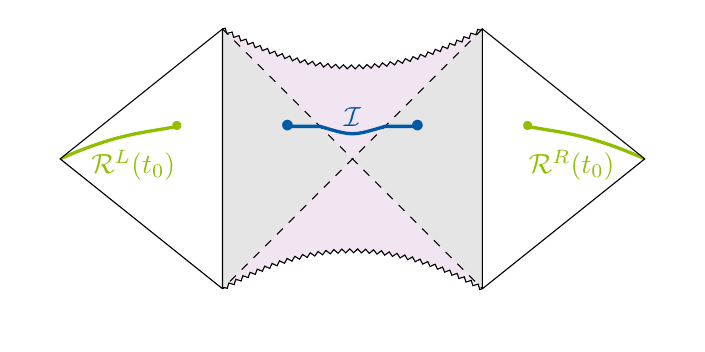
\begin{tikzpicture}[scale=1.65]
\node at (1.35,0.25) {\textcolor{black!25!lime}{\footnotesize$\bullet$}};
\draw[-,black!25!lime,very thick] (1.35,0.25)  .. controls (1.6,0.2) and (1.8,0.2) ..  (2.25,0);
\draw[-,draw=none,fill=white] (1,1) to (2.25,0) to (2.5,0) to (1.25,1) to (1,1);


\node at (-1.35,0.25) {\textcolor{black!25!lime}{\footnotesize$\bullet$}};
\draw[-,black!25!lime,very thick] (-1.35,0.25) .. controls (-1.6,0.2) and (-1.8,0.2) .. (-2.25,0);
\draw[-,draw=none,fill=white] (-1,1) to (-2.25,0) to (-2.5,0) to (-1.25,1) to (-1,1);


\node at (3.375/2,-0.05) {\textcolor{black!25!lime}{$\mathcal{R}^R(t_0)$}};
\node at (-3.375/2,-0.05) {\textcolor{black!25!lime}{$\mathcal{R}^L(t_0)$}};



\draw[-,draw=none,fill=black!10] (1,1) to (1,-1) to (0,0) to (1,1); 
\draw[-,draw=none,fill=black!10] (-1,1) to (-1,-1) to (0,0) to (-1,1);

\draw[-,draw=none,fill=violet!10] (-1,1) to[bend right] (1,1) to (0,0) to (-1,1); 
\draw[-,draw=none,fill=violet!10] (1,-1) to[bend right] (-1,-1) to (0,0) to (1,-1);

\draw[-,decoration = {zigzag,segment length = 1mm, amplitude = 0.25mm},decorate] (-1,1) to[bend right] (1,1);
\draw[-] (1,1) to (1,-1);
\draw[-,decoration = {zigzag,segment length = 1mm, amplitude = 0.25mm},decorate] (1,-1) to[bend right] (-1,-1);
\draw[-] (-1,-1) to (-1,1);

\draw[-,dashed] (-1,1) to (1,-1);
\draw[-,dashed] (1,1) to (-1,-1);

\draw[-] (1,-1) to (2.25,0) to (1,1) to (1,-1);
\draw[-] (-1,-1) to (-2.25,0) to (-1,1) to (-1,-1);


\draw[-,very thick,blue!30!teal] (-0.5,0.25) to (-0.25,0.25) .. controls (0,0.175) .. (0.25,0.25) to (0.5,0.25);
\node[blue!30!teal] at (-0.5,0.25) {$\bullet$};
\node[blue!30!teal] at (0.5,0.25) {$\bullet$};

\node[blue!30!teal] at (0,0.325) {$\mathcal{I}$};
\node at (0,-1.2) {};
\end{tikzpicture}
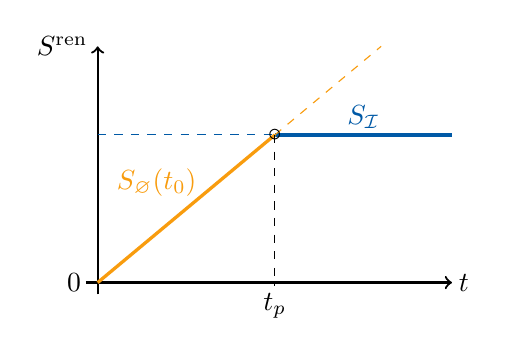
\begin{tikzpicture}[scale=0.75]
\draw[->,thick] (0,-0.2) to (0,4);
\draw[->,thick] (-0.2,0) to (6,0);

\node at (-0.6,4) {$S^{\text{ren}}$};
\node at (6.2,0) {$t$};

\draw[-,blue!30!teal,very thick] (3,2.5) to (6,2.5);
\draw[-,dashed,blue!30!teal] (0,2.5) to (3,2.5);

\draw[-,dashed,yellow!20!orange] (3,2.5) to (4.8,4);
\draw[-,yellow!20!orange,very thick] (0,0) to (3,2.5);
\node at (3,2.5) {$\circ$};
\draw[-,dashed] (3,2.5) to (3,0);
\draw[-] (3,0) to (3,-0.05);
\node at (3,-0.4) {$t_p$};


\node[yellow!20!orange] at (1,1.7) {$S_\varnothing(t_0)$};
\node[blue!30!teal] at (4.5,2.8) {$S_{\mathcal{I}}$};

\node at (-0.4,0) {$0$};
\end{tikzpicture}
\caption{On the left is the two-sided thermal configuration of (II) featuring both the $t = t_0$ radiation region $\mathcal{R}^L(t_0) \cup \mathcal{R}^R(t_0)$ and the island $\mathcal{I}$ which emerges at late times. The right figure is a sketch of the (eternal) Page curve depicting (renormalized) entanglement entropy versus time---initially the time-dependent no-island entropy $S_\varnothing$ is minimal, but it eventually exceeds the non-trivial island entropy $S_{\mathcal{I}}$. This curve can be obtained by computing (renormalized) areas in the (III) configuration.}
\label{figs:eternalBH}
\end{figure}

In (III), following the RT prescription without regarding the islands---that is for $\mathcal{I} = \varnothing$---tells us that \textit{Hartman-Maldacena surfaces} encode the entanglement entropy of radiation \cite{Hartman:2013qma}. In satisfying the homology constraint, these spacelike surfaces cross the interior of the AdS$_{d+1}$ black hole's Einstein-Rosen bridge. The entropy thus exhibits monotonic growth from $t = 0$, with the late-time $t \gg \beta$ growth being linear. This eternal growth is an information paradox in (II)---the Hawking radiation becomes more entropic than even the black hole \cite{Almheiri:2019yqk}.

This issue is resolved if nontrivial islands are considered. In particular, \cite{Almheiri:2019yqk} discusses how the minimal entropy after the \textit{Page time} $t = t_p$ counts an entanglement island which goes outside of the black hole interior, so at $t = t_p$ there is a phase transition. This is explicitly seen by a classical computation in (III) if we compare the Hartman-Maldacena area---a time-dependent quantity---to the area of a minimized extremal surface residing solely outside of the interior and ending on the brane---a time-independent quantity. The resulting late-time entropy is thus constant, as found by \cite{Almheiri:2019yqk}. This means that the Page curve is indeed encoded by the semiclassical picture in which gravity resides on the brane and radiation escapes into a bath.

Note that this phase transition depicted in the eternal Page curve (Figure \ref{figs:eternalBH}) is analogous to the typical Hartman-Maldacena phase transition seen with no branes \cite{Hartman:2013qma}. With no branes, we have an RT surface which is entirely homologous to the boundary interval and in the exterior, so this surface would bound the late-time entropy and produce the same sort of entropy curve. In fact, the setup with the tensionless brane is precisely a $\mathbb{Z}_2$ orbifold \cite{Shashi:2020mkd,Geng:2020qvw}, and so the phase transition of interest is literally the one of Hartman and Maldacena when interpreted in the bulk (as opposed to one which is informed by some nontrivial extremal surface boundary condition at the brane).

Nonetheless, the important interpretation is that of the braneworld theory (II), not the bulk theory (III). The former is where we may view this entropy curve as corresponding to a phase transition of quantum extremal surfaces \cite{Engelhardt:2014gca}, while the latter is simply a classical phase transition.

As an aside, the comparison can be done entirely on the $t = 0$ slice, for which there is no interior contribution to a Hartman-Maldacena surface's area. Fixing the endpoints of $\mathcal{R}^L$ and $\mathcal{R}^R$ to be the same distance from the brane, one can find whether or not the island surface is already minimal at $t = 0$ \cite{Geng:2020qvw}---this would imply no phase transition and no Page curve. In doing so, one finds that the radiation region cannot be too close to the brane to get a Page curve (see Section \ref{sec3.1}).

\subsection{Massive Gravity from the Bath}

All of this begs the question---to what extent does the coupling of an external bath influence the story? Previous work has explored the effect of the graviton mass. It is known that in $d \geq 4$, by coupling the $AdS_d$ brane to a bath with a transparent boundary condition at the interface, the localized gravitational theory on the brane becomes a theory of massive gravity with no massless graviton \cite{Aharony:2003qf,Aharony:2006hz}. In \cite{Geng:2020qvw} the authors tuned the near-zero mass down, finding that the nontrivial island candidate surface grows in response. This limit is essentially performed by tuning the tension of the brane up towards its critical value; in response however, the brane's cosmological constant $\Lambda_b$ and dynamical gravity on the brane turns off. A way out which preserves the massless graviton and dynamical gravity was found by \cite{Krishnan:2020fer}, which puts the critical brane at a cutoff surface in the AdS$_{d+1}$ bulk to keep $G_d$ finite. This procedure saves the islands for $d = 2$, although whether it works for $d > 2$ remains to be seen.\footnote{The case of $d > 2$ would \textit{also} need to be reconciled with \cite{Geng:2021gau}, which argues for incompatibility between islands and massless gravitons in $d > 2$ using the Hamiltonian constraints of gravity.}

A different way to introduce a zero-mass graviton \cite{Geng:2020fxl} is to make the bath itself \textit{gravitating}, but this gives a \textit{constant} entropy curve if we follow a dynamical\footnote{Here, ``dynamical" simply means that the higher-dimensional classical island surface has Neumann boundary conditions on both branes.} island rule---a result in agreement with \cite{Laddha:2020kvp}. Note however that there is disagreement in the literature on whether the flat curve of \cite{Laddha:2020kvp,Geng:2020fxl} actually depicts the appropriate entropy for a black hole in the first place; \cite{Krishnan:2020oun} argues for a different factorization from \cite{Laddha:2020kvp} as being relevant to the radiating black hole while \cite{Ghosh:2021axl} uses the gravitating bath of \cite{Geng:2020fxl} with alternate (Dirichlet) boundary conditions for the island surface. \cite{Krishnan:2020oun,Ghosh:2021axl} both find Page curves in their respective analyses, with the presence of a bath potentially muddying the picture of how one should factorize.

Differences in the literature and pending questions aside, a lot can be learned by either slightly deviating from or further probing the typical ``brane and nongravitating half-space BCFT bath" construction, as done by \cite{Caceres:2020jcn,Anderson:2021vof,Bhattacharya:2021jrn,Ghosh:2021axl,Geng:2021iyq,Qi:2021sxb,Geng:2021eps}.

\subsection{Deforming the Bath}

In this work we pursue a different way of altering (although not eliminating) the nongravitating bath: we study a bath deformation corresponding to a scalar field in the bulk and explore how it affects the Page curve. With no branes, it is known that introducing a scalar deformation on the conformal boundary of an AdS black hole will change the near-singularity geometry from AdS-Schwarzschild to a \textit{Kasner universe} \cite{Kasner:1921zz,Belinski:1973zz,Das:2006dz,Frenkel:2020ysx}. The Kasner universe metric is essentially that of the Schwarzschild geometry but with some extra warp factors. Up to pre-factors and in $d+1$ bulk dimensions ($d \geq 2$), the near-singularity geometry and scalar field behave as (restricting to isotropic gravity + scalar solutions), 
\begin{equation}
ds^2 \sim -d\tau^2 + \tau^{2p_t}dt^2 + \tau^{2p_x} d\vec{x}^2,\ \ \phi(r) \sim -\sqrt{2} p_\phi \log\tau,\label{kasMet}
\end{equation}
where $\tau,t \in \mathbb{R}$, $\vec{x} \in \mathbb{R}^{d-1}$, and $p_t,p_x,p_\phi$ are the \textit{Kasner exponents}. These exponents obey a set of constraints,
\begin{align}
p_t + (d-1)p_x &= 1,\label{exp1}\\
p_\phi^2 + p_t^2 + (d-1)p_x^2 &= 1,\label{exp2}
\end{align}
so there is only one free exponent.

Notably, these exponents affect the \textit{entanglement velocity}---the speed of the late-time linear growth of the Hartman-Maldacena surface spanning the interior. As this is also the early-time entanglement surface when a brane is present, it is natural to think that the Page curve and, in particular, the Page time will also change.\footnote{There is a subtlety regarding $d = 2$ when adding a brane: the lowest order terms in the brane's induced gravity action are a nondynamical Einstein-Hilbert term and a nonlocal Polyakov $R\log|R|$ term \cite{Chen:2020uac}. As we are assuming an effective dynamical description on the brane, any of our statements about Page curves only work for $d > 2$.}

The deformed geometries studied by \cite{Frenkel:2020ysx} are called \textit{Kasner flows} because, from the holographic RG flow program \cite{Balasubramanian:1999jd}, the scalar deformation induces an RG flow from a UV fixed point state on the conformal boundary to a late-time singularity in the black hole's interior \cite{Kiritsis:2016kog,Gursoy:2018umf}, with the scaling changing from spacelike to timelike at the horizon. Thus as mentioned above, the flow is to an IR state at the horizon then gets analytically-continued to a trans-IR flow towards the Kasner universe.

The flows are labeled by a dimensionless parameter on the boundary. Each of these flows thus describes a particular coarse-graining of the UV state, controlled by a corresponding radial scale $r_{\text{RG}}$ which is probed by the Hartman-Maldacena surface. This scale is roughly defined such that the UV physics dominates between the conformal boundary and $r_{\text{RG}}$, while the IR/trans-IR physics becomes more important between the singularity and $r_{\text{RG}}$. Concretely, we get a more rapidly coarse-grained state as $r_{\text{RG}}$ approaches the boundary.

Upon adding a brane, each flow becomes one of a BCFT thermal state \cite{Rozali:2019day,Sato:2020upl}, and we must account for the island surface. This introduces an independent radial scale $r_T$---the intersection depth of the island surface with the brane---which is directly determined by the metric functions and the size of the radiation region $\mathcal{R}$. This radial scale is tied to how many bath degrees of freedom we trace out when directly computing the entropy of Hawking radiation. It is thus related to the ``dynamics" of the entanglement entropy; a larger $r_T$ corresponds to tracing-out more degrees of freedom and thus a higher saturation value of the entropy.

From this perspective, when adding a brane the resulting Page curves found by the island rule probe both the coarse-graining and the entanglement dynamics. Purely from a BCFT perspective, we would heuristically expect two things: (1) that strong IR effects in the bath should increase the Page time by decreasing the $c_{\rm bulk}$ \cite{Rozali:2019day} and (2) that the dynamical part of the Page curve can only be seen after integrating away a minimum number of degrees of freedom. We indeed find both to be the case at least within the numerical range we explore.


%%%%%%%%%%%%%%%%%%%%%%%%

%%%%%%%%%%%%%%%%%
\section{Kasner Flows as AdS/CFT Solutions}\label{sec2}
%%%%%%%%%%%%%%%%%

We start with a review of the Kasner flows, following \cite{Frenkel:2020ysx} but generalizing their equations. We take $(d+1)$-dimensional Einstein gravity ($d \geq 2$) with negative cosmological constant $\Lambda = -d(d-1)/2$ (setting the AdS radius to $1$) and coupled to a scalar field $\phi$ with potential $V(\phi)$. With $16\pi G_{d+1} = 1$, the action is,
\begin{equation}
I = \int d^{d+1}x \sqrt{-g}\left(R + d(d-1) - \frac{1}{2}\left[\nabla^\alpha\phi \nabla_\alpha\phi + V(\phi)\right]\right).\label{action}
\end{equation}
As in \cite{Frenkel:2020ysx}, we consider the minimal case of a free massive scalar field---the potential being $V(\phi) = m^2 \phi^2$. Note that the flows solving this action with an additional higher-order $\lambda\phi^4$ coupling have been studied by \cite{Wang:2020nkd}.

The bulk equations of motion are the usual Einstein + scalar equations and the Klein-Gordon equations (defining $\square = \nabla_\alpha \nabla^\alpha$),
\begin{align}
G_{\mu\nu} - \frac{d(d-1)}{2}g_{\mu\nu} &= \frac{1}{4}\left[2\nabla_\mu \phi \nabla_\nu \phi - g_{\mu\nu}\left(\nabla^\alpha \phi \nabla_\alpha \phi + m^2\phi^2\right)\right],\\
(\square - m^2)\phi &= 0,
\end{align}
For the metric, we take solutions of the form,
\begin{equation}
ds^2 = \frac{1}{r^2}\left[-f(r)e^{-\chi(r)} dt^2 + \frac{dr^2}{f(r)} + d\vec{x}^2\right],\label{metAnsatz}
\end{equation}
where $t \in \mathbb{R}$, $r > 0$, and $\vec{x} \in \mathbb{R}^{d-1}$. For $\phi$, we consider a radial ansatz: $\phi = \phi(r)$. The dual scalar operator $\mathcal{O}$ is then a constant boundary deformation. By the AdS/CFT dictionary \cite{Aharony:1999ti}, its conformal dimension $\Delta$ satisfies a mass-dimension relation,
\begin{equation}
m^2 = \Delta(\Delta - d).\label{massdimension}
\end{equation}
Plugging this into the Klein-Gordon equation and combining the result with the $tt$ and $rr$ components of the Einstein + scalar equations yields a set of ODEs,
\begin{align}
\phi'' + \left(\frac{f'}{f} - \frac{d-1}{r} - \frac{\chi'}{2}\right)\phi' + \frac{\Delta(d-\Delta)}{r^2 f}\phi& = 0,\label{eom1}\\
\chi' - \frac{2f'}{f} - \frac{\Delta(d-\Delta)\phi^2}{(d-1)rf} - \frac{2d}{rf} + \frac{2d}{r} &= 0,\label{eom2}\\
\chi' - \frac{r}{d-1}\left(\phi'\right)^2 &= 0,\label{eom3}
\end{align}
in agreement with \cite{Frenkel:2020ysx} when $d = 3$ and $m^2 = -2$.

We are concerned with black holes, so we suppose that $f$ has a simple root at $r = r_+$---this is the horizon. Furthermore while the conformal boundary is located at $r = 0$, the singularity in our coordinates is at $r = \infty$. We must also have regularity of the metric \eqref{metAnsatz} at the horizon. To emphasize this point, we note the existence of infalling coordinates in which the metric takes the form,
\begin{equation}
ds^2 = \frac{1}{r^2}\left[-f(r) e^{-\chi(r)} du^2 + 2e^{-\chi(r)/2} du\,dr + d\vec{x}^2\right].
\end{equation}
Lastly observe that the above ansatz with a particular choice of the radial functions becomes the AdS-Schwarzschild black hole---take $f(r) = 1-(r/r_+)^{d}$ and $\chi(r) = 0$. The equations of motion (specifically \eqref{eom2}) then imply,
\begin{equation}
\phi(r) = 0,
\end{equation}
so AdS-Schwarzschild is indeed the vacuum solution with no backreaction from $\phi$.

We now describe the asymptotic behavior of the radial functions as well as the corresponding field theoretic data both near the UV boundary theory ($r \to 0$) and near the IR singularity theory ($r \to \infty$). Additionally we discuss how the bulk represents an RG flow from one to the other, allowing us to treat the near-singularity data as emergent from the near-boundary data.

%%%%%%%%%%%%%%%%%
\subsection{Near-Boundary Expressions and Data}\label{sec2.1}
%%%%%%%%%%%%%%%%%

The near-boundary ($r \to 0$) expressions are standard to AdS/CFT. While there is some subtlety upon which we expand in Appendix \ref{appA}, the key point is that a relevant scalar operator with conformal dimension $\Delta < d$ is precisely dual to a bulk scalar field with negative $m^2$ but satisfying the \textit{Breitenlohner-Freedman stability bound} \cite{Breitenlohner:1982bm},
\begin{equation}
-\frac{d^2}{4} \leq m^2 < 0.
\end{equation}
However, we restrict to operator dimension above the unitarity bound,
\begin{equation}
\Delta \geq \frac{d-2}{2}.
\end{equation}
Thus for any value of $m^2$ between $-d^2/4$ and $1-d^2/4$, the mass-dimension relation \eqref{massdimension} gives us two possibilities for $\Delta$ depending on the boundary conditions of $\phi$ \cite{Klebanov:1999tb,Minces:1999eg}.\footnote{For the edge case $m^2 = -d^2/4$, we only consider the Dirichlet boundary condition to avoid a double root in the CFT two-point function when taking $\Delta = d/2$.} \cite{Frenkel:2020ysx} uses the ``canonical" quantization in which the larger candidate (which is more strictly bounded from below by $d/2$) is chosen, but we can still take any $\Delta$ above the unitarity bound. While the bulk equations of motion are only sensitive to $m^2$, this choice will affect our interpretations of the leading-order and next-to-leading-order modes in the near-boundary expressions.

With that in mind, we now write the $\Delta \neq d/2$ near-boundary mode expansion of the field $\phi(r)$ in terms of the boundary \textit{source} $\phi_0$ and the \textit{one-point function} $\expval{\mathcal{O}}$,
\begin{equation}
\phi(r) \sim \phi_0 r^{d-\Delta} + \frac{\expval{\mathcal{O}}}{2\Delta - d}r^{\Delta}.\label{fieldBdry}
\end{equation}
Next, we use the fall-off of the $tt$ component of the metric to write,
\begin{equation}
-r^2 g_{tt} = f(r)e^{-\chi(r)} \sim 1 - \expval{T_{tt}}r^d,\label{fg}
\end{equation}
where $\expval{T_{tt}}$ is the \textit{energy density} of the thermal state. These expressions are enough to write the near-boundary expansion of $\chi(r)$ by plugging into the equation of motion \eqref{eom3} and noting that $\chi(0) = 0$,
\begin{equation}
\begin{split}
\chi(r) \sim\ &\frac{d-\Delta}{2(d-1)}\phi_0^2 r^{2(d-\Delta)} + \frac{2\Delta(d-\Delta)}{d(d-1)(2\Delta - d)}\phi_0 \expval{\mathcal{O}} r^d\\
&+ \frac{\Delta}{2(d-1)(2\Delta-d)^2}\expval{\mathcal{O}}^2 r^{2\Delta}.
\end{split}
\end{equation}
For $\Delta = d/2$ however, while we still have \eqref{fg}, we now write the Dirichlet expression \cite{Minces:1999eg},
\begin{equation}
\phi(r) \sim \phi_0 r^{d/2}\log r,
\end{equation}
and integrating the differential equation \eqref{eom3} yields,
\begin{equation}
\chi(r) \sim \frac{\phi_0^2}{4d(d-1)} r^d \left[2 + 2d\log r + d^2 (\log r)^2\right].
\end{equation}
There is one more aspect of the boundary state left---the temperature $T$. Because \eqref{metAnsatz} is time-independent, we may easily compute the surface gravity $\kappa$ to get $T$. Defining $\vec{K} = \partial_t$, $f_+' = f'(r_+)$ (nonzero by assumption), and $\chi_+ = \chi(r_+)$,
\begin{equation}
T = \frac{\kappa}{2\pi} = \left.\frac{1}{2\pi}\sqrt{-\frac{1}{2}(\nabla^\alpha K^\beta)(\nabla_\alpha K_\beta)}\right|_{r = r_+} = \frac{|f'_+|e^{-\chi_+/2}}{4\pi}.\label{tempDef}
\end{equation}
Imposing regularity on the radial functions at the horizon, the near-boundary data---$\expval{T_{tt}}$ and $\expval{\mathcal{O}}$ in particular---can be written in terms of the dimensionless ratio $\phi_0/T^{d-\Delta}$---the \textit{deformation parameter}. As this data determines the rest of the bulk geometry by the equations of motion, the entire holographic RG flow (for each $d$ and $\Delta$ and including the near-singularity data in the IR) is labeled by $\phi_0/T^{d-\Delta}$.

%%%%%%%%%%%%%%%%%
\subsection{Near-Singularity Expressions and Data}\label{sec2.2}
%%%%%%%%%%%%%%%%%

We now write the near-singularity ($r \to \infty$) expressions for the radial functions. The scalar field is dominated by a logarithmic divergence \cite{Doroshkevich:1978aq,Fournodavlos:2018lrk} which we write as,
\begin{equation}
\phi(r) \sim (d-1) c\log r.\label{singField}
\end{equation}
Here $c$ is a constant with $c = 0$ corresponding to the Schwarzschild solution to the Einstein + scalar theory. Plugging this into \eqref{eom3} yields the near-singularity behavior of $\chi$,
\begin{equation}
\chi(r) \sim (d-1)c^2 \log r + \chi_1,
\end{equation}
where $\chi_1$ is a constant. We then use the remaining equations of motion to write $f$, bearing in mind that it is negative in the interior.
\begin{equation}
f(r) \sim -f_1 r^\rho,\ \ \rho = d + \left(\frac{d-1}{2}\right)c^2.
\end{equation}
Note that these expressions all coincide with \cite{Frenkel:2020ysx} at $d = 3$. Plugging these into the metric \eqref{metAnsatz} and reparameterizing the now-timelike radial coordinate as,
\begin{equation}
r = \tau^{-2/\rho},
\end{equation}
yields (up to rescalings of the spacelike coordinates and an overall factor) the Kasner universe and corresponding scalar field \eqref{kasMet},
\begin{equation}
ds^2 \sim -d\tau^2 + \tau^{2p_t} dt^2 + \tau^{2p_x} d\vec{x}^2,\ \ \phi(\tau) \sim -\sqrt{2} p_\phi\log\tau,
\end{equation}
with the Kasner exponents being (in terms of $\rho$),
\begin{equation}
p_t = 1 - \frac{2(d-1)}{\rho},\ \ p_x = \frac{2}{\rho},\ \ p_\phi = \frac{2\sqrt{(d-1)(\rho-d)}}{\rho}.
\end{equation}
These indeed satisfy the Kasner constraints \eqref{exp1} and \eqref{exp2}. Furthermore at the Schwarzschild value $c = 0 \implies \rho = d$, we get,
\begin{equation}
\text{Schwarzschild:}\ \ p_t = -1 + \frac{2}{d},\ \ p_x = \frac{2}{d},\ \ p_\phi = 0.
\end{equation}


%%%%%%%%%%%%%%%%%
\subsection{Emergent Kasner Exponents from Flow}\label{sec2.3}
%%%%%%%%%%%%%%%%%

\begin{table}
\centering
\begin{tabular}{c||c|c}{}
& Near-boundary ($r \to 0$) & Near-singularity ($r \to \infty$)\\\hline\hline & & \vspace{-1em}\\
$\underset{(\Delta \neq d/2)}{\phi(r)}$ & $\phi_0 r^{d-\Delta} + \dfrac{\expval{\mathcal{O}}}{2\Delta - d} r^\Delta$ & $\sqrt{2(d-1)(\rho - d)}\log r$\\ & & \vspace{-1em}\\ \hline & &\vspace{-1em}\\
$\underset{(\Delta = d/2)}{\phi(r)}$ & $\phi_0 r^{d/2}\log r$ & $\sqrt{2(d-1)(\rho - d)}\log r$\\ & & \vspace{-1em}\\ \hline & &\vspace{-1em}\\
$\underset{(\Delta \neq d/2)}{\chi(r)}$ & $\dfrac{d-\Delta}{2(d-1)}\phi_0^2 r^{2(d-\Delta)} + \dfrac{2\Delta(d-\Delta)}{d(d-1)(2\Delta - d)}\phi_0\expval{\mathcal{O}}r^d$ & $2(\rho-d) \log r + \chi_1$\\
& $ \qquad\qquad\qquad\qquad+ \dfrac{\Delta}{2(d-1)(2\Delta-d)^2}\expval{\mathcal{O}}^2 r^{2\Delta}$ & \\ & & \vspace{-1em}\\ \hline & &\vspace{-1em}\\
$\underset{(\Delta = d/2)}{\chi(r)}$ & $\dfrac{\phi_0^2}{4d(d-1)} r^d \left[2 + 2d\log r + d^2 (\log r)^2\right]$ & $2(\rho-d) \log r + \chi_1$\\ & & \vspace{-1em}\\ \hline & &\vspace{-1em}\\
$f(r)$ & $e^{\chi(r)}\left(1 - \expval{T_{tt}}r^d\right)$ & $-f_1 r^{\rho}$
\end{tabular}
\caption{The near-boundary and near-singularity expressions for the radial functions characterizing a Kasner flow ansatz for the Einstein + scalar theory. The near-boundary data is controlled by the deformation parameter $\phi_0/T^{d-\Delta}$ while all of the near-singularity data is determined by the Kasner exponent $p_t$.}
\label{tables:asymptoticExpressions}
\end{table}

We summarize the results of Sections \ref{sec2.1} and \ref{sec2.2} in Table \ref{tables:asymptoticExpressions}. While these results seem disconnected, we now discuss how these different asymptotic limits are linked by the bulk RG flow.

From studying the near-boundary and near-singularity data, we have that, independently of the holographic RG flow, the former is fixed by $\phi_0/T^{d-\Delta}$ while the latter is fixed by any one of the Kasner exponents---we use $p_t$ as done in \cite{Frenkel:2020ysx,Wang:2020nkd}. However, when equipped with both the near-boundary data and the equations of motion, the entire flow is already fixed and thus sets a value for $p_t$. Thus the Kasner exponents are emergent from the deformation parameter and the flow.

The most concrete way to examine this relationship is to plot the value of $p_t$ as a function of $\phi_0/T^{d-\Delta}$. For the Einstein + scalar theory, we do so for various dimensions in Figure \ref{figs:kasnerVsDef}. These plots are numerically determined, requiring $d$ and $\Delta$ as inputs. The details of our methodology are discussed in Appendix \ref{appB}.
{
\floatsetup[figure]{style=plain,subcapbesideposition=center}
\begin{figure}
\centering
\sidesubfloat[$d=2$]{
\includegraphics[scale=0.75]{figs/kasnerVsDef/kasnerVsDefd2.pdf}
}\\\vspace{0.4cm}
\sidesubfloat[$d=3$]{
\includegraphics[scale=0.75]{figs/kasnerVsDef/kasnerVsDefd3.pdf}
}\\\vspace{0.4cm}
\sidesubfloat[$d=4$]{
\includegraphics[scale=0.75]{figs/kasnerVsDef/kasnerVsDefd4.pdf}
}
\caption{The emergent Kasner exponent $p_t$ versus the dimensionless deformation parameter $\phi_0/T^{d-\Delta}$ for various $d$ and $\Delta$, computed via a numerical shooting method outlined in Appendix \ref{appB}. We show the results for (a) $d = 2$, (b) $d = 3$, and (c) $d = 4$. The dashed lines correspond to $\Delta = d/2$.}
\label{figs:kasnerVsDef}
\end{figure}
}

While the numerical values depend on $d$---even the exactly-known Schwazrschild value for $p_t$ depends on dimension---the qualitative behavior of the emergent $p_t$ appears to satisfy an inversion-like symmetry. Specifically there is a value of $\phi_0/T^{d-\Delta}$ for which $p_t$ is maximized, whereas $\phi_0/T^{d-\Delta} \to \infty$ appears to give the Schwarzschild value.\footnote{This is also stated by \cite{Frenkel:2020ysx,Wang:2020nkd}, but it is not immediate from the plots. Rather, this is assumed asymptotic behavior based on running the numerics to large $\phi_0/T^{d-\Delta}$.} However there is still a problem of fine-tuning---it is unclear how the maximum is actually set. As a preliminary observation, the numerics indicate that the corresponding $\Delta = \Delta_+$ and $\Delta = \Delta_-$ (same $m^2$) flows attain the same maximum $p_t$.

The work done in a self-interacting scalar theory \cite{Wang:2020nkd} finds the qualitative behavior to hold more generally, but the fine-tuning problem persists---the value and location of the maximum depends on the details of the theory. How these flows may exhibit universal behavior is an interesting open question which we intend to revisit.

%%%%%%%%%%%%%%%%%
\section{Page Curves as Probes of Flows}\label{sec3}
%%%%%%%%%%%%%%%%%

Taking \eqref{metAnsatz}, we add a \textit{Karch-Randall (KR) brane} and excise space beyond it. We then study the entanglement surfaces in the resulting geometry. Before discussing the details however, we briefly review the set-up (also discussed in the Introduction).

We consider the action \eqref{action} with an additional term (with $16\pi G_{d+1} = 1$),
\begin{equation}
I_{RS} = 2\int_{\mathcal{Q}} d^dx \sqrt{-h}(K-T_{RS}).
\end{equation}
$\mathcal{Q}$ is a \textit{Randall-Sundrum (RS) brane} with tension $T_{RS}$, induced metric $h_{ab}$, and extrinsic curvature $K_{ab}$. In RSII models characterized by end-of-the-world branes, $\mathcal{Q}$ is the boundary of a manifold solving \eqref{action} and satisfying a Neumann condition,
\begin{equation}
K_{ab} = (K-T_{RS})h_{ab}.\label{neumannBrane}
\end{equation}
With no scalar field, $\mathcal{Q}$ is a KR brane specifically when the induced geometry is AdS$_d$. This occurs precisely when the tension is \textit{subcritical}, satisfying the bound,
\begin{equation}
|T_{RS}| < d-1.\label{critical}
\end{equation}
In practice, we find such KR branes by taking some foliation of AdS$_{d+1}$ into AdS$_d$ slices, then computing their respective tensions \cite{Aharony:2003qf}. However in our work, we are considering (scalar) backreacted geometries, so the induced geometry on the brane is not a vacuum solution. Nonetheless we still have a KR brane so long as we find a boundary for which \eqref{neumannBrane} is satisfied.
%\pagebreak
\FloatBarrier

Einstein gravity in the bulk ``localizes" to ``induced" quantum gravity on the brane \cite{Karch:2000ct,Karch:2000gx,Chen:2020uac}, although what localization means is a matter of interpretation. Agnostically, the original Karch-Randall story \cite{Karch:2000ct} considers the transverse-traceless (TT) modes of linearized fluctuations arising from the backreaction of the brane. Generically, these TT modes satisfy the Schr\"odinger equation with a ``volcano" potential containing a weighted $\delta$-function term centered at the brane (see Figure \ref{figs:volcanoPotential}). However, the weight of the $\delta$-function smoothly vanishes as $T_{RS} \to 0$ (i.e. the probe limit), resulting in the loss of the volcano's ``crater." Regardless of the tension however, solving for the KK tower of spin-2 modes becomes a quantum mechanics problem---computing the eigenstates (labeled by their masses) of the Schr\"odinger equation with the volcano potential.

In the near-critical-tension regime when \eqref{critical} is nearly saturated, the lowest-mass (``almost-zero") mode has a positive mass which is nonetheless much smaller than the masses in the rest of the tower \cite{Karch:2000ct,Miemiec:2000eq,Schwartz:2000ip}. Furthermore, the almost-zero mode's wavefunction is sharply peaked at the brane. Thus we think of the almost-zero KK mode as a graviton that is ``localized" to the brane in the sense of its wavefunction dying off quickly in the bulk. The higher modes meanwhile dualize to a CFT on the brane. This gives description (II) in the Introduction for the near-critical branes.

However, we remark that there is not necessarily a problem with maintaining this interpretation as we leave the critical limit. As we tune the tension down by $O(1)$ factors, the mass spacing between the almost-zero mode and the first excited state will decrease, and the former's corresponding wavefunction will broaden. In other words, the almost-zero mode no longer has an obvious interpretation as a localized graviton. Nonetheless, these changes are quantitative rather than qualitative, and there is no sign of a discontinuity in the bulk analysis. Thus, one may advocate (as we do so here) that viewing the almost-zero mode as a graviton coupled to a CFT obtained from the higher modes is still a valid holographic interpretation of the picture.\footnote{We thank Andreas Karch for clarifying this point and its corresponding rationale to us.} Indeed, \cite{Almheiri:2019psy} considers such a scenario at a tension which is certainly subcritical.\footnote{\cite{Almheiri:2019psy} considers $d = 4$. The critical tension is $3$, but they use a brane with tension $3/\sqrt{2}$.} However, the theory of gravity here would be far more unusual than in the near-critical limit in that there is stronger mixing between the graviton and the CFT, since the states of the KK tower are all ``closer together."

\begin{figure}
\centering
\includegraphics[scale=0.85]{figs/volcanoPot.pdf}
\caption{A sketch of the AdS volcano potential $V(w)$ in \cite{Karch:2000ct} for $d = 4$, depicted as a function of a coordinate $w$ which is normal to the brane. We show both the $T > 0$ case (which has a crater) and the $T = 0$ case (which lacks a crater).}
\label{figs:volcanoPotential}
\end{figure}

The fine-tuning which pushes the limits of this reasoning the most is the tensionless case, in which we lack both the almost-zero-mode wavefunction's sharp peak and, as stated above and shown in Figure \ref{figs:volcanoPotential}, the crater of the volcano potential. Both features might be viewed as signals of ``localization." However, there is still no discontinuity when going from nonzero to zero tension; indeed, the crater vanishes smoothly as seen in the volcano potential written in \cite{Karch:2000ct} for $d = 4$. Along the reasoning of \cite{Geng:2020fxl} (which, as we do here, studies entanglement islands), the tensionless braneworld theory is then ``no worse" than that of nonzero tension, at least away from the near-critical regime.
%\sanjit{End of new paragraph}

With dynamical gravity on the brane, the conformal boundary acts as a ``bath" into which information may flow from the brane theory. We thus have a natural arena in which to explore black hole information---simply put a black hole on the brane itself. Furthermore as we have a scalar deformation on the bath controlled by $\phi_0/T^{d-\Delta}$, we can observe how tuning the deformation affects information.

To further take a semiclassical approximation, we consider the leading-order effective induced action---identified as $d$-dimensional Einstein gravity from the series worked out by \cite{Chen:2020uac}. The induced Einstein action is dynamical for $d > 2$ but not for $d = 2$ (for which having a dynamical effective theory would require inclusion of the next-to-leading order Polyakov term $\sim R\log|R|$). We thus only consider $d > 2$ and leave explorations of the relationship between scalar deformations and Page curves in $d = 2$ to future work.

Concretely, we compute holographic entanglement entropy. We assume that the appropriate semiclassical holographic prescription is still the island rule \cite{Penington:2019npb,Almheiri:2019psf,Almheiri:2019hni,Almheiri:2020cfm} but in the backreacted geometry---for some radiation region $\mathcal{R}$ on the boundary as shown in Figure \ref{figs:islands}, its entanglement entropy to leading order as $G_{d+1} \to 0$ is given as,
\begin{equation}
S(\mathcal{R}) = \frac{A(\gamma)}{4G_{d+1}},\label{islandRuleInduced}
\end{equation}
Here $\gamma$ is the minimal-area surface in the island rule, so it can either be entirely homologous to $\mathcal{R}$ or be homologous to $\mathcal{R} \cup \mathcal{I}$ where $\mathcal{I}$ is an entanglement island residing on the brane. We specifically study two-sided black holes, so the radiation region consists of a left piece $\mathcal{R}^L$ and right piece $\mathcal{R}^R$ as in Figure \ref{figs:eternalBH}.

%\sanjit{start of new paragraph}
Using \eqref{islandRuleInduced} however requires fixing a particular KR brane and thus setting a tension $T_{RS}$. For mathematical simplicity, we consider the probe limit $T_{RS} = 0$; islands with nonzero tension have been studied by \cite{Almheiri:2019psy,Geng:2020qvw,Geng:2020fxl,Chen:2020uac,Chen:2020hmv} but we leave how this part of the story interacts with scalar deformations of the bath open to exploration. We also reiterate that, although the holographic interpretation of the tensionless ``brane + bath" theory is highly nonstandard gravity due to the lack of separation between the almost-zero and excited spin-2 KK modes, in following \cite{Geng:2020fxl} we proceed on the basis of this scenario being not particularly worse than those of nonzero-tension braneworlds.
%\sanjit{End of new paragraph}

Regarding the position of the brane, picking-out a transverse coordinate $x^1$ in $\vec{x} = (x^1,...,x^{d-1})$ as shown in the metric \eqref{metAnsatz}, we take the slice,
\begin{equation}
x^1 = 0.\label{probeBrane}
\end{equation}
We must ensure that this is a proper KR brane---that given the full action \eqref{action} plus the RS term, both the geometry \eqref{metAnsatz} and the radial scalar field ansatz $\phi = \phi(r)$ discussed in Section \ref{sec2} satisfy boundary conditions on $\mathcal{Q}$. Starting with the former, we note that the normal unit vector is,
\begin{equation}
n_\mu = \frac{1}{r}\delta_{\mu 1},
\end{equation}
where $\delta_{\mu 1}$ is the Kronecker delta and $1$ denotes the $x^1$ coordinate. The resulting extrinsic curvature on the \eqref{probeBrane} slice is then,
\begin{equation}
K_{ab} = 0,
\end{equation}
so this is certainly a tensionless KR brane.

As for the scalar field $\phi = \phi(r)$, it clearly satisfies a Neumann boundary condition because it is independent of $x^1$,
\begin{equation}
n^\mu \partial_\mu \phi(r) = r \partial_1 \phi(r) = 0.
\end{equation}
The punchline is that, for a particular scalar deformation---that is some deformation parameter $\phi_0/T^{d-\Delta}$---there exist radiation regions for which the entanglement entropy between the left and right parts of a two-sided black hole with a KR brane obeys a Page curve (Figure \ref{figs:eternalBH}). There are technically three parameters which can be tuned given $d$: $\phi_0/T^{d-\Delta}$, the operator dimension $\Delta$, and the endpoint of the radiation region $x_\mathcal{R}$ (on both sides---we take $\mathcal{R}^L$ and $\mathcal{R}^R$ to start at $x^1 = x_\mathcal{R}$).

The primary parameter of interest is $\phi_0/T^{d-\Delta}$ because, by keeping $\Delta$ and $x_\mathcal{R}$ fixed, the resulting Page curves correspond directly to bulk RG flows from the same equations of motion. We also study how changing $\Delta$ affects the Page curve. The underlying motivation behind this analysis is to understand how changing the bath deformation may alter the physics, so we leave $x_\mathcal{R}$ alone (although we need to justify that such a radiation region which can be kept stable despite tuning the deformation indeed exists---see Section \ref{sec3.1} for details).

Nonetheless, it is also interesting to understand what happens when we tune $x_\mathcal{R}$. To do so meaningfully, we fix $d = 3$ and $\Delta = 2$, comparing the AdS-Schwarzschild solution ($\phi_0/T = 0$) to a solution for a nontrivial deformation. We find that larger $x_\mathcal{R}$ correspond to more direct probes of backreaction in the interior specifically.

%%%%%%%%%%%%%%%%%
\subsection{The Page Point}\label{sec3.1}
%%%%%%%%%%%%%%%%%

When tuning the scalar deformation, a natural question arises: can we definitively choose a radiation region $\mathcal{R}$ which yields a Page curve regardless of the values of $\phi_0/T^{d-\Delta}$ and $\Delta$? We thus define the \textit{Page point} $x_p$ as the value of $x_\mathcal{R}$ for which,
\begin{align}
0 \leq x_\mathcal{R} \leq x_p &\implies \text{no Page curve for }S(\mathcal{R}),\\
x_\mathcal{R} > x_p &\implies \text{Page curve for }S(\mathcal{R}).
\end{align}
The analysis below essentially follows \cite{Geng:2020qvw} but for a probe brane \eqref{probeBrane}, general blackening factor $f(r)$, and various dimensions. \cite{Geng:2020qvw} confirms the existence of Page points in AdS-Schwarzschild for $d = 4$.

Specifically, we restrict our attention to the $t = 0$ slice on which the interior is trivial. Given some radiation region, we will ultimately find two candidates for the entanglement surface (Figure \ref{figs:candidateSurfaces}): Hartman-Maldacena surfaces \cite{Hartman:2013qma} which span the black hole without hitting the brane and \textit{island surfaces} which hit the brane outside of the horizon \cite{Almheiri:2019yqk}. The Hartman-Maldacena surfaces grow away from the $t = 0$ slice because of the growth in the Einstein-Rosen bridge, whereas the island surfaces are time-independent and thus maintain a constant area.

\begin{figure}
\centering
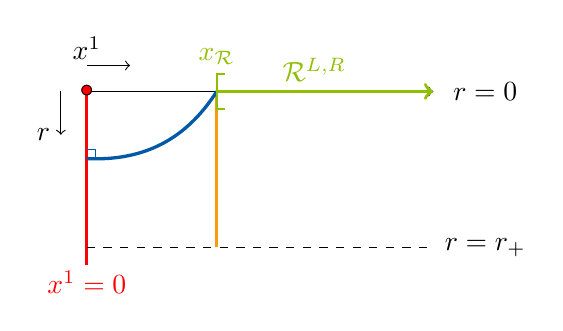
\begin{tikzpicture}[scale=1.1]
\draw[->] (0,2) to (2+2,2);
\draw[-,very thick,red] (0,2) to (0,0);

\draw[->] (0,2.3) to (0.5,2.3);
\node at (0,2.5) {$x^1$};

\draw[->] (-0.3,2) to (-0.3,1.5);
\node at (-0.5,1.5) {$r$};

\node at (0,-0.2) {\textcolor{red}{$x^1 = 0$}};

\draw[-,dashed] (0,0.2) to (2+2,0.2);

\node at (2+2.6,0.2) {$r = r_+$};
\node at (2+2.6,2) {$r = 0$};

\draw[-,yellow!20!orange,very thick] (1.5,2) to (1.5,0.2);
\draw[-,blue!30!teal,very thick] (1.5,2) to[bend left] (0,1.225);
\draw[-,blue!30!teal] (0.1,1.225) to (0.1,1.325) to (0,1.325);

\draw[->,very thick,black!25!lime] (1.5,2) to (4,2);
\node at (2.625,2.25) {\textcolor{black!25!lime}{$\mathcal{R}^{L,R}$}};

\draw[-,black!25!lime,thick] (1.6,2.2) to (1.5,2.2) to (1.5,1.8) to (1.6,1.8);
\node at (1.5,2.4) {\textcolor{black!25!lime}{$x_\mathcal{R}$}};

\node[color=red] at (0,2) {$\bullet$};
\node at (0,2) {$\circ$};
\end{tikzpicture}
\caption{The candidate RT surfaces in one of the exterior regions. The orange line entering the horizon is the Hartman-Maldacena surface, whereas the blue arc which ends perpendicularly on the brane is the island-producing exterior surface.}
\label{figs:candidateSurfaces}
\end{figure}

For a particular radiation region defined by $x_\mathcal{R}$, we can identify which of these surfaces is ``initially" minimal and deduce whether or not we get a Page curve---this happens if the Hartman-Maldacena surface is minimal at $t = 0$.\footnote{Note that in our calculations, we will be computing the portions of the area in just one of the exterior patches and multiplying by $2$ to get the $t = 0$ areas.} We will ultimately compute the Page point for various dimensions as a function of $\phi_0/T^{d-\Delta}$.

Jumping into the calculation, the geometry of the $t = 0$ slice is,
\begin{equation}
ds^2|_{t=0} = \frac{1}{r^2}\left[\frac{dr^2}{f(r)} + d\vec{x}^2\right] = \frac{1}{r^2}\left[\frac{dr^2}{f(r)} + \sum_{i=1}^{d-1} (dx^i)^2\right].
\end{equation}
Parameterizing an arbitrary surface as $x^1 = x^1(r)$, its area functional is,
\begin{equation}
A = \int dx^2 \cdots dx^{d-1} \int \frac{dr}{r^{d-1}}\sqrt{\frac{1}{f(r)} + \dot{x}^1(r)^2},\ \ \dot{x}^1 = \frac{dx^1}{dr}.
\end{equation}
Integrating over $(x^2,...,x^{d-1})$ produces an overall volume factor $V_{d-2}$ which is irrelevant when comparing different surfaces $x^1(r)$ together, so we only care about the \textit{area density} (also called ``area" for convenience) $\mathcal{A}$ and its Lagrangian $\mathcal{L}$,
\begin{equation}
\mathcal{A} = \frac{A}{V_{d-2}} = \int \frac{dr}{r^{d-1}}\sqrt{\frac{1}{f(r)} + \dot{x}^1(r)^2} = \int dr\,\mathcal{L}.\label{area}
\end{equation}
We want to minimize $\mathcal{A}$. The Euler-Lagrange equations indicate that $\partial\mathcal{L}/\partial\dot{x}^1$ is a constant of motion. In fact, defining the \textit{turnaround point} $r = r_T > 0$ as the root of $1/\dot{x}^1(r)$ (so $dr/dx^1 = 0$ here), we have that minimal surfaces satisfy,
\begin{equation}
\frac{\dot{x}^1(r)}{r^{d-1}\sqrt{\frac{1}{f(r)} + \dot{x}^1(r)^2}} = \pm\frac{1}{r_{T}^{d-1}} \implies \dot{x}^1(r) = \pm\frac{r^{d-1}}{\sqrt{f(r)\left[r_T^{2(d-1)} - r^{2(d-1)}\right]}}.\label{solutionsMinimal}
\end{equation}
These surfaces must also satisfy boundary conditions at the conformal boundary ($r = 0$) and at the brane ($x^1 = 0$). Because of the branching in \eqref{solutionsMinimal}, the conditions must be derived by assuming a more general parameterization $(r(s),x^1(s))$ with $s \in [0,1]$ \cite{Geng:2020fxl}. They are respectively a Dirichlet condition and a Neumann condition,
\begin{align}
\text{Boundary:}&\ \ x^1(0) = x_\mathcal{R},\\
\text{Brane:}&\ \ \left.\frac{1}{\dot{x}^1(r)}\right|_{x^1 = 0} = 0.
\end{align}
So for some $x_\mathcal{R}$, the minimal surfaces in the presence of a probe brane are those which satisfy \eqref{solutionsMinimal} and either do not end on the brane (Hartman-Maldacena),
\begin{equation}
r_T = \infty \implies x^1(r) = x_\mathcal{R},
\end{equation}
or do end on the brane (island surfaces). For the latter case, the turnaround point is precisely along the brane, i.e.,\footnote{These statements come from viewing the tensionless braneworld as orbifolded AdS$_{d+1}$ \cite{Shashi:2020mkd,Geng:2020qvw}.}
\begin{equation}
x^1(r_T) = 0,
\end{equation}
but the above equations of motion constrain the value of $r_T$ to depend on $x_\mathcal{R}$. Specifically by integrating \eqref{solutionsMinimal} (noting that the only branch which reaches the brane from $x_\mathcal{R} > 0$ is the negative one), we have,
\begin{equation}
\int_0^{r_T}dr \frac{r^{d-1}}{\sqrt{f(r)\left[r_T^{2(d-1)} - r^{2(d-1)}\right]}} = x_\mathcal{R}.\label{radEnd}
\end{equation}
We now use \eqref{area} to write the $t = 0$ areas of both the Hartman-Maldacena surface and the island surface given some $x_\mathcal{R}$. Respectively they are (taking the area in one exterior patch and multiplying by $2$),
\begin{align}
\mathcal{A}_{HM}(0) &= 2\int_0^{r_+} \frac{dr}{r^{d-1}\sqrt{f(r)}},\label{hm0}\\
\mathcal{A}_I &= 2\int_0^{r_T} \frac{dr}{r^{d-1}\sqrt{f(r)}} \frac{r_T^{d-1}}{\sqrt{r_T^{2(d-1)} - r^{2(d-1)}}}.
\end{align}
Both of these are divergent at the boundary, so we will need to renormalize them. We use the standard holographic renormalization---integrating from a cutoff $r/r_+ = \epsilon \ll 1$ then adding the appropriate counterterm before taking $\epsilon \to 0$. For both of these areas, the integrands go to $1/r^{d-1}$ as $r \to 0$, so the counterterm is the same as for areas in empty AdS$_{d+1}$ and only depends on the dimension,
\begin{equation}
r_+^{d-2} \mathcal{A}_{CT} = -\dfrac{2}{(d-2)}\dfrac{1}{\epsilon^{d-2}}.\label{areaCT}
\end{equation}
While this is important for evaluating Page curves, in determining whether or not there is a Page curve to begin with we only need to use the area difference,
\begin{equation}
\begin{split}
\Delta\mathcal{A}(0)
=\ &\mathcal{A}_I - \mathcal{A}_{HM}(0)\\
=\ &2\int_0^{r_T} \frac{dr}{r^{d-1}\sqrt{f(r)}} \left[\frac{r_T^{d-1} - \sqrt{r_{T}^{2(d-1)} - r^{2(d-1)}}}{\sqrt{r_T^{2(d-1)} - r^{2(d-1)}}}\right] -2\int_{r_T}^{r_+} \frac{dr}{r^{d-1}\sqrt{f(r)}},
\end{split}\label{areaDiff}
\end{equation}
which is UV-finite. There is then a Page curve if and only if $\Delta\mathcal{A}(0) > 0$.

\begin{figure}
\centering
\subfloat[Area difference]{
\includegraphics[scale=0.4]{figs/pagePointAS/areaDiffAdSSchwarzschild.pdf}}\qquad
\subfloat[Page point]{
\includegraphics[scale=0.4]{figs/pagePointAS/pagePointAdSSchwarzschild.pdf}}
\caption{(a) The area difference $\Delta\mathcal{A}(0)$ \eqref{areaDiff} versus $x_\mathcal{R}$ \eqref{radEnd} for $d = 3,4,5$ and (b) the Page point $x_p$ as a function of (analytically-continued) $d > 2$, all in the AdS-Schwarzschild geometry and in $r_+$ units. The area difference in each dimension monotonically increases with $x_\mathcal{R}$, crossing $0$ at a particular value beyond which we have Page curves. The Page point thus approaches the brane as we increase $d$.}
\label{figs:pagePointAS}
\end{figure}
{
\floatsetup[figure]{style=plain,subcapbesideposition=center}
\begin{figure}
\centering
%\sidesubfloat[$d=2$]{\includegraphics[scale=1]{figs/pagePointKasner/pagePointd2.pdf}}\\\vspace{0.4cm}
\sidesubfloat[$d=3$]{\includegraphics[scale=0.27]{figs/pagePointKasner/pagePointd3.pdf}}\\\vspace{0.4cm}
\sidesubfloat[$d=4$]{\hspace{-0.1cm}\includegraphics[scale=0.27]{figs/pagePointKasner/pagePointd4.pdf}}
\caption{The Page point $x_p$ as a function of $\phi_0/T^{d-\Delta}$ for (a) $d = 3$ and (b) $d = 4$ (the cases in Section \ref{sec3.2}). The horizontal lines are at the AdS-Schwarzschild Page points shown in Figure \ref{figs:pagePointAS}. The Page point decreases as $\phi_0/T^{d-\Delta}$ increases.}
\label{figs:pagePointKasner}
\end{figure}
}


If we have AdS-Schwarzschild---that is $f(r) = 1 - (r/r_+)^d$---then it is straightforward to plot $\Delta\mathcal{A}(0)$ as a function of $x_\mathcal{R}$ using \eqref{radEnd} and \eqref{areaDiff}. We do this for various dimension in Figure \ref{figs:pagePointAS}, thus finding the Page points $x_p$ in such geometries. Numerically, these Page points (in dimensionless coordinates) for $d = 3,4$ are,
\begin{equation}
\frac{x_p}{r_+} \approx \begin{cases}
0.589,&\text{if}\ d = 3,\\
0.444,&\text{if}\ d = 4.
\end{cases}
\end{equation}
We now extend this analysis to nonzero $\phi_0/T^{d-\Delta}$---increasing the deformation parameter changes $f(r)$ and thus the calculation of $\mathcal{A}$. We again utilize a shooting method, this time numerically solving for $f(r)$ in the exterior. Doing so allows us to compute the Page points in a particular $d$ as a function of $\phi_0/T^{d-\Delta}$ (Figure \ref{figs:pagePointKasner}).


Observe that the Page point decreases as we increase $\phi_0/T^{d-\Delta}$---a large scalar deformation results in Page curves for larger radiation regions. Notably, if we take a radiation region $x_\mathcal{R}> x_p$ with zero deformation (i.e. in AdS-Schwarzschild), then we may tune $\phi_0/T^{d-\Delta}$ up while keeping $x_\mathcal{R}$ fixed without losing the Page curve. This justifies the viewpoint of our work---that the Page curves for a particular radiation region probe Kasner flows.

%%%%%%%%%%%%%%%%%
\subsection{Entanglement Entropy and Page Curves}\label{sec3.2}
%%%%%%%%%%%%%%%%%

We now compute the Page curves for various dimensions $d$ and conformal dimensions $\Delta$. To reiterate, the endpoint $x_{\mathcal{R}}$ of the radiation region is also a tunable parameter, but in studying the effect of changing the scalar deformation we start by keeping it fixed. For much of the analysis below, we will assume,
\begin{equation}
x_{\mathcal{R}} = 2x_p,\label{radRegionFix}
\end{equation}
which ensures that we always have a Page curve with finite Page time. We subsequently briefly touch on the physics of increasing $x_\mathcal{R}$.

However, while the island surfaces are constant in time, the Hartman-Maldacena surfaces are not---we merely know them to be constant-$x^1$ surfaces. In Section \ref{sec3.1} we computed the areas of these surfaces at $t = 0$, so we now consider the areas as functions of time. Only then can we plot the Page curves themselves.

%\FloatBarrier

%%%%%%%%%%%%%%%%%
\subsubsection{Growth of the Hartman-Maldacena Surfaces}\label{sec3.2.1}
%%%%%%%%%%%%%%%%%

The procedure for computing the time-dependent Hartman-Maldacena surfaces is outlined by \cite{Hartman:2013qma}. Since the analysis in this particular section is blind to KR branes, we include $d = 2$ here. For a constant-$x^1$ slice,\footnote{The analysis below is blind to which constant-$x^1$ slice we take.} the induced metric from \eqref{metAnsatz} is,
\begin{equation}
ds^2|_{x^1 = x_{\mathcal{R}}} = \frac{1}{r^2}\left[-f(r)e^{-\chi(r)} dt^2 + \frac{dr^2}{f(r)} + \sum_{i=2}^{d-1} (dx^i)^2\right].
\end{equation}
%\FloatBarrier


\noindent For a surface $r = r(t)$, the area functional is then,
\begin{equation}
A = V_{d-2}\int \frac{dt}{r(t)^{d-1}} \sqrt{-f[r(t)] e^{-\chi[r(t)]} + \frac{\dot{r}(t)^2}{f[r(t)]}},\ \ \dot{r} = \frac{dr}{dt},\label{areaTimeInt}
\end{equation}
with the area (density) functional and corresponding Lagrangian being,
\begin{equation}
\mathcal{A}= \int \frac{dt}{r(t)^{d-1}} \sqrt{-f[r(t)] e^{-\chi[r(t)]} + \frac{\dot{r}(t)^2}{f[r(t)]}} = \int dt\,\mathcal{L}.\label{timeArea}
\end{equation}
The lack of explicit $t$-dependence in this Lagrangian gives us a constant of motion which we identify as the ``energy" $E$ of the minimal surface (suppressing $t$),
\begin{equation}
E = \dot{r}\pdv{\mathcal{L}}{\dot{r}} - \mathcal{L} = \frac{f(r)e^{-\chi(r)}}{r^{d-1}\sqrt{-f(r)e^{-\chi(r)} + \frac{\dot{r}^2}{f(r)}}},
\end{equation}
so the minimal trajectories are defined by,
\begin{equation}
\dot{r} = \pm f(r)e^{-\chi(r)/2}\sqrt{1+\frac{f(r)e^{-\chi(r)}}{(r^{d-1}E)^2}}.\label{hmBranches}
\end{equation}
We may conventionally take the sign of $E$ to match the sign of \eqref{hmBranches}. Now observe that $\dot{r} = 0$ in the interior (when $f < 0$) if there is a radius $r = r_{*}$ such that,
\begin{equation}
-\frac{f(r_*)e^{-\chi(r_*)}}{r_*^{2(d-1)}} = E^2.\label{energyRStar}
\end{equation}
So for a surface with such an energy $E$, this is the maximal value of $r$ assumed. In full, the surface starts at the conformal boundary, reaches $r = r_*$, then goes to the other side of the black hole. Thus (reparameterizing as $t = t(r)$ and using $dt/dr = 1/\dot{r}$), we have that the area is,
\begin{equation}
\mathcal{A}_{HM}(t_b) = 2\int_0^{r_*} \frac{dr}{r^{d-1}\sqrt{f(r) + e^{\chi(r)}(r^{d-1}E)^2}} \implies \dot{r}|_{r = r_*} = 0.
\end{equation}
Here, we refer to the Hartman-Maldacena area as being a function of the \textit{boundary time} $t_b$. This is to avoid confusion with the bulk time coordinate.\footnote{The specific case of $t_b = 0$ coincides exactly with the analysis on the $t = 0$ slice. We can confirm this by noting that the corresponding energy is $E = 0$.} We find it by considering the integral,
\begin{equation}
\int_0^{r_*} \frac{dr}{\dot{r}} = t_* - t_b,
\end{equation}
which computes the time difference between $t_b$ and $t_* = t(r_*)$. By restricting our attention to \textit{symmetric} surfaces---those for which $t_*$ is purely imaginary---we get the boundary time in terms of $E$ \cite{Frenkel:2020ysx} (removing the pole at the horizon),
\begin{equation}
t_b = -P\int_0^{r_*} \frac{\text{sgn}(E) e^{\chi/2}}{f(r)\sqrt{1 + f(r)e^{-\chi(r)}/(r^{d-1}E)^2}}.
\end{equation}
To summarize, $E$ is a parameter for the Hartman-Maldacena surfaces which determines the maximal radius $r_*$, the boundary time $t_b$, and the area $\mathcal{A}_{HM}$. We restrict consideration to $E \geq 0$---this keeps us in the $t_b \geq 0$ regime.

To conclude this discussion, we analyze the late-time ($t_b \to \infty$) behavior of these surfaces. It is first necessary to observe that the function,
\begin{equation}
g(r) = -\frac{f(r)e^{-\chi(r)}}{r^{2(d-1)}},
\end{equation}
has a maximum at some \textit{critical radius} $r = r_c$ in the interior. This is because,\footnote{This argument breaks down for $d = 2$ in AdS-Schwarzschild---$c = 0$ and thus $\rho = 2$. Instead, the ``maximum" is at infinity, so we take $r_c = \infty$. The late-time Hartman-Maldacena surfaces here are thus geodesics which probe the singularity itself.}
\begin{equation}
g(r_+) = 0,\ \ \lim_{r \to \infty} g(r) = \lim_{r \to \infty} f_1 e^{-\chi_1} r^{-(\rho - 2)} = 0,\ \ g(r)|_{r > r_+} > 0.
\end{equation}
We have used the asymptotic expressions for $f$ and $\chi$ (Table \ref{tables:asymptoticExpressions}). Denoting the corresponding energy for the surface with $r_* = r_c$ by $E = E_c$, \eqref{energyRStar} indicates that,
\begin{equation}
1 + \frac{f(r_c)e^{-\chi(r_c)}}{(r_c^{d-1}E_c)^2} = 0,
\end{equation}
so the integral for the boundary time diverges, i.e. $t_b \to \infty$ as $r_* \to r_c$. This surface is in a sense the ``maximal" one.

Now by plugging into \eqref{timeArea} as in \cite{Hartman:2013qma}, we can obtain the linear-growth term for $\mathcal{A}_{HM}$ and hence for the entanglement entropy $S = V_{d-2}\mathcal{A}_{HM}/(4G_{d+1})$. Specifically for late boundary times, we use the integrand to write,\footnote{When writing the late-time linear behavior of entropy, one typically uses an \textit{entropy density} $s$ in conjunction with the transverse volume. We find it to be $\sim 2/r_+^{d-1}$.}
\begin{equation}
\pdv{\mathcal{A}_{HM}}{t_b} = -2 \frac{f(r_c)e^{-\chi(r_c)}}{r_c^{2(d-1)}} \frac{1}{|E_c|} = 2\sqrt{-\frac{f(r_c) e^{-\chi(r_c)}}{r_{c}^{2(d-1)}}} = \frac{2v}{r_{+}^{d-1}},\label{eVel}
\end{equation}
where $v$ is the entanglement velocity---a dimensionless factor which captures the speed of entropy growth---as written by \cite{Frenkel:2020ysx}. In AdS-Schwarzschild \cite{Hartman:2013qma},
\begin{equation}
v_{AS} = \frac{\sqrt{d}(d-2)^{(d-2)/(2d)}}{[2(d-1)]^{(d-1)/d}}.\label{velocityAS}
\end{equation}
\cite{Frenkel:2020ysx} plots $v$ in the Kasner metric in terms of $p_t$ for $d = 3$, $\Delta = 2$. As we care about boundary data, we present analogous plots for various $d$ and $\Delta$ in Figure \ref{figs:entanglementVelocity}.

{
\floatsetup[figure]{style=plain,subcapbesideposition=center}
\begin{figure}
\centering
\sidesubfloat[]{\hspace{0.11cm}\includegraphics[scale=0.55]{figs/entanglementVelocities/vspt/velVsptd2.pdf}\hspace{-0.3cm} \includegraphics[scale=0.5375]{figs/entanglementVelocities/vsphi0/velVsphi0d2.pdf}}\\\vspace{0.4cm}
\sidesubfloat[]{\hspace{0.09cm}\includegraphics[scale=0.55]{figs/entanglementVelocities/vspt/velVsptd3.pdf}\hspace{-0.3cm} \includegraphics[scale=0.5465]{figs/entanglementVelocities/vsphi0/velVsphi0d3.pdf}}\\\vspace{0.4cm}
\sidesubfloat[]{\hspace{-0.01cm}\includegraphics[scale=0.562]{figs/entanglementVelocities/vspt/velVsptd4.pdf}\hspace{-0.315cm} \includegraphics[scale=0.539]{figs/entanglementVelocities/vsphi0/velVsphi0d4.pdf}}
\caption{Entanglement velocity $v$ as a function of $p_t$ and $\phi_0/T^{d-\Delta}$ for (a) $d = 2$, (b) $d = 3$, and (c) $d = 4$. Each plot starts at its AdS-Schwarzschild value from \eqref{velocityAS}. The $p_t$ curves obey a $\Delta \leftrightarrow d-\Delta$ symmetry---they are sensitive to $m^2$.}
\label{figs:entanglementVelocity}
\end{figure}
}

For all relevant deformations used in our numerics---including $\Delta > d/2$, $\Delta < d/2$, and $\Delta = d/2$---as a function of $\phi_0/T^{d-\Delta}$ the entanglement velocity decreases from the AdS-Schwarzschild value $v_{AS}$ until reaching a minimal value, then slowly increases back towards $v_{AS}$. This is much like what we see in the behavior of the Kasner exponent $p_t$ (Figure \ref{figs:kasnerVsDef}). Essentially this indicates a nontrivial relationship between the scalar deformation and the ``speed" of entanglement in the bath.

Regarding the Page time, we still need to compare the Hartman-Maldacena surfaces to the island surfaces. These also change under the scalar deformation but additionally depend on $x_\mathcal{R}$ (whereas the Hartman-Maldacena surfaces alone do not).



%%%%%%%%%%%%%%%%%
\subsubsection{Initial Area Difference and the Page Time}\label{sec3.2.2}
%%%%%%%%%%%%%%%%%

We are now equipped to compute Page curves given some $d$, $\Delta$, and $x_\mathcal{R}$ (returning to the KR model and $d > 2$). As we wish to understand the physics of the scalar deformation, we first keep the radiation region fixed at $x_\mathcal{R}= 2 x_p$ \eqref{radRegionFix}, thus ensuring a Page curve regardless of the deformation. We present our numerics in terms of the area and boundary time in units of $r_+$.

As a preliminary exercise, we numerically compute the Page curve for $d = 3$, $\Delta = 2$ for both $\phi_0/T = 0$ and $\phi_0/T \approx 35.0$ (the latter being close to the minimum for $v$). To do so, we simply use the expressions from Section \ref{sec3.2.1} to acquire the entropy from the Hartman-Maldacena surface and those of Section \ref{sec3.1} to get its upper bound---the entropy from the island surface. We renormalize both of the areas using the standard counterterm \eqref{areaCT}. The result is shown in Figure \ref{figs:pageCurveEx}.

\begin{figure}
\includegraphics[scale=0.425]{figs/pageCurveExample.pdf}
\caption{The Page curves for $\phi_0/T = 0$ and $\phi_0/T \approx 35.0$ with $d = 3$, $\Delta = 2$, presented in terms of the area $\mathcal{A}$ and boundary time $t_b$ in units of $r_+$. The orange curves are Hartman-Maldacena surface areas while the blue curves are island surface areas. For both, we observe a phase transition from the former to the latter at finite boundary times---the respective Page times given these deformations.}
\label{figs:pageCurveEx}
\end{figure}

To confirm that our numerics are appropriately tuned, we perform two checks. The first is to compare the initial area $r_+^{d-2} \mathcal{A}_{HM}(0)$ of the $\phi_0/T = 0$ curve to the analytical result (Appendix \ref{appC}). Indeed for $d = 3$, we have,
\begin{equation}
r_+^{d-2}\mathcal{A}_{HM}(0)|_{\phi_0/T = 0} = -\frac{2\sqrt{\pi}\Gamma\left(\frac{2}{3}\right)}{\Gamma\left(\frac{1}{6}\right)} \approx -0.862,
\end{equation}
which closely aligns with Figure \ref{figs:pageCurveEx}.

The second check is to compare the entanglement velocities (found from halving the late-time slope of the Hartman-Maldacena surface areas \eqref{eVel}) against both each other and the values seen in previous sections. According to our numerics,
\begin{equation}
v|_{\phi_0/T = 0} \approx 0.687,\ \ v|_{\phi_0/T \approx 35.0} \approx 0.653.
\end{equation}
These match Figure \ref{figs:entanglementVelocity}, with $v|_{\phi_0/T = 0}$ also being the AdS-Schwarzschild value found from \eqref{velocityAS}.

Observe that the entanglement velocity is not the only thing which changes---the scalar deformation also affects the initial difference $\Delta\mathcal{A}(0)$ between the Hartman-Maldacena and island surfaces to O$(10^{-1})$,
\begin{equation}
\Delta\mathcal{A}(0)|_{\phi_0/T = 0} \approx 1.43,\ \ \Delta\mathcal{A}(0)|_{\phi_0/T \approx 35.0} \approx 1.72.
\end{equation}
Furthermore the Page times read from Figure \ref{figs:pageCurveEx} are,
\begin{equation}
\left.\frac{t_p}{r_+}\right|_{\phi_0/T = 0} \approx 1.34,\ \ \left.\frac{t_p}{r_+}\right|_{\phi_0/T \approx 35.0} \approx 1.52.
\end{equation}
Indeed, we may ask which effect is more significant in influencing the Page time: the change to the entanglement velocity or the change to the area difference. Assuming linear behavior by the Hartman-Maldacena area---a loose but apparently safe approximation within $t_b/r_+ \sim O(1)$---we can estimate the Page time as,
\begin{equation}
t_p \approx \frac{\Delta\mathcal{A}(0)}{2v},
\end{equation}
so the ``first-order" variation in the Page time $\delta t_p$ is related to the variations in initial area difference and entanglement velocity by,
\begin{equation}
\delta t_p \approx \frac{\delta(\Delta\mathcal{A}(0))}{2v} - \frac{\Delta\mathcal{A}(0)}{2v^2} \delta v.\label{varTP}
\end{equation}
So for the numbers above and using the average values of $\Delta\mathcal{A}(0)$ and $v$, this estimation yields (writing both terms individually and setting $r_+ = 1$),
\begin{equation}
\delta t_p \approx 0.22 + 0.06 = 0.28.
\end{equation}
The point is not exactness, but to demonstrate that the contribution from $\delta(\Delta\mathcal{A}(0))$ (of $O(10^{-1})$) is more significant than the contribution from $\delta v$ (of $O(10^{-2})$. The former comes from backreaction in the exterior while the latter comes from backreaction in the interior. As our numerics indicate that $\delta t_p$ is actually closer to $0.19 \sim O(10^{-1})$, it is the former effect---the exterior backreaction---which has a greater influence on the Page time.

To obtain a more complete picture, we numerically compute two additional sets of plots, expanding our analysis to $d = 3,4$ and a range of $\Delta$. The first set is the initial area difference $\Delta \mathcal{A}(0)$ as a function of $\phi_0/T^{d-\Delta}$. The second is the Page time $t_p$ as a function of $\phi_0/T^{d-\Delta}$. We present our results in Figure \ref{figs:areasAndPageTimes}.

{
\floatsetup[figure]{style=plain,subcapbesideposition=center}
\begin{figure}
\centering
\sidesubfloat[]{\hspace{-0.02cm}\includegraphics[scale=0.335]{figs/areasAndPageTimes/3dAreaDiff.pdf}\hspace{0.3cm} \includegraphics[scale=0.35]{figs/areasAndPageTimes/3dPageTime.pdf}}\\\vspace{0.4cm}
\sidesubfloat[]{\hspace{-0.07cm}\includegraphics[scale=0.335]{figs/areasAndPageTimes/4dAreaDiff.pdf}\hspace{0.3cm} \includegraphics[scale=0.343]{figs/areasAndPageTimes/4dPageTime.pdf}}
\caption{The initial area difference $\Delta\mathcal{A}(0)$ and the Page time $t_p$ plotted as functions of $\phi_0/T^{d-\Delta}$ for (a) $d = 3$ and (b) $d = 4$, all for various $\Delta$. The axes are in $r_+$ units.}
\label{figs:areasAndPageTimes}
\end{figure}
}

The numerics are unstable at larger values of $\phi_0/T^{d-\Delta}$, which is why we restrict to $\sim 1500$. In spite of this limitation, there are lessons in how the plots for different $\Delta$ relate to one another. Firstly, the $\phi_0/T^{d-\Delta} = 0$ values---when the deformation is turned off---has no dependence on $\Delta$. There is no backreaction and thus, unsurprisingly, the geometry is just AdS-Schwarzschild.

For all $\Delta$, as we increase the deformation parameter both the initial area and the Page time grow, seemingly together with the range of variation being $O(10^{-1})$. This is evidence for the statement above: the changes to the entanglement velocity are so small that it is indeed the changes to the initial area difference which more strongly inform the changes in the Page time.

Noteworthy is the large $\phi_0/T^{d-\Delta}$ behavior. The Page time $t_p/r_+$ curves in particular appear to fall into two ``families" of behavior---the $\Delta < d/2$ curves (corresponding to the ``Neumann" $\Delta = \Delta_-$ quantization) and the $\Delta \geq d/2$ curves (corresponding to the ``Dirichlet" $\Delta = \Delta_+$ quantization)\footnote{We reiterate that there technically exists a Neumann $\Delta = d/2$ quantization which we do not include here.} seem to separate from another. This is most evident for the Page time plot in $d = 4$, in which the curves in the same family actually approach one another.

Taking this behavior seriously, we may claim that upon introducing a large scalar deformation, the Page time is not sensitive to $\Delta$---only the quantization (as viewed by \cite{Klebanov:1999tb}) of the deformation, which we recall is related to the boundary condition of the scalar field \cite{Minces:1999eg}.

%%%%%%%%%%%%%%%%%
\subsubsection{Interior Versus Exterior Backreaction}\label{sec3.2.3}
%%%%%%%%%%%%%%%%%

In the previous section we present our results across a variety of $d$ and $\Delta$ but keeping $x_\mathcal{R}$ fixed at twice the Page point $x_p$. While we were able to probe the effect of simply tuning the deformation on the Page time, we found that the exterior backreaction influenced the quantitative results more than the interior backreaction. We thus now keep $d = 3$ and $\Delta = 2$, again comparing $\phi_0/T = 0$ to $\phi_0/T \approx 35.0$ but tuning $x_\mathcal{R}$.

The numbers of interest are the variation in the initial area difference and the variation in the Page time. Respectively we recall them to be,
\begin{align}
\delta(\Delta\mathcal{A}(0))
&= \Delta\mathcal{A}(0)|_{\phi_0/T \approx 35.0} - \Delta\mathcal{A}(0)|_{\phi_0/T = 0},\\
\delta t_p
&= t_p|_{\phi_0/T \approx 35.0} - t_p|_{\phi_0/T = 0},
\end{align}
and these are plotted as functions of $x_\mathcal{R}$ (in units of $r_+$) in Figure \ref{figs:variationRadEnd}.

\begin{figure}
\centering
\subfloat[Variation in initial area difference]{
\includegraphics[scale=0.45]{figs/variationRadEnd/areaVariation.pdf}}\qquad
\subfloat[Variation in Page time]{
\includegraphics[scale=0.45]{figs/variationRadEnd/pageTimeVariation.pdf}}
\caption{The variations in the (a) initial area difference and the (b) Page time as functions of the radiation region. We compute these quantities up to $x_\mathcal{R}/x_p = 6$, at which point our numerics become too noisy to be taken as reliable. Nonetheless, even within this range the numerics indicate that the variation in initial area difference monotonically falls while the variation in the Page time drops then rises.}
\label{figs:variationRadEnd}
\end{figure}

We again look at \eqref{varTP} in $r_+ = 1$ units. To reiterate, the variation in the initial area surface can be thought of as coming from the backreaction in the exterior, whereas $\delta v$---the variation in entanglement velocity---comes from the backreaction of the interior. For $x_\mathcal{R} \approx x_p$, the first term is much closer to the order of $\delta t_p$ than the second term. This is seen in our previous analysis and again in the early part of the plots in Figure \ref{figs:variationRadEnd}.

However, taking the behavior in Figure \ref{figs:variationRadEnd} seriously would indicate that $\delta(\Delta\mathcal{A}(0))$ remains $O(10^{-1})$ even as $x_\mathcal{R} \gg x_p$, whereas $\delta t_p$ increases and is eventually orders of magnitude larger. \eqref{varTP} would imply that the $\delta v$ term is responsible---specifically the initial area difference $\Delta\mathcal{A}(0)$ itself is what grows and thus more heavily weights the effect of $\delta v$ on $\delta t_p$.

Physically, we interpret this is as the existence of two regimes: $x_\mathcal{R} \approx x_p$ in which the exterior backreaction plays a significant, leading-order role in determining the Page time and $x_\mathcal{R} \gg x_p$ in which the interior backreaction has a stronger influence on Page time. Nonetheless these numerics still indicate that, regardless of the regime of $x_\mathcal{R}$, the Page time with a scalar deformation is longer than with no scalar deformation.

%%%%%%%%%%%%%%%%%%%%%%%%%%%%%%%%%%%%%%%%
\section{Conclusions and Outlook} %%%%%%
%%%%%%%%%%%%%%%%%%%%%%%%%%%%%%%%%%%%%%%%

In this paper, we use a doubly holographic setup to investigate the effect of a bath deformation on the fine-grained entanglement dynamics of a gravitating black hole. We add a relevant scalar operator in the bath and study the change of the Page curve, Page point, and Page time as functions of the deformation parameter $\phi_0/T^{d-\Delta}$. Performing two analyses, we find the following:
\begin{itemize}
\item[(1)] Keeping the radiation region $\mathcal{R}$ fixed, we increase the deformation parameter and find, within our numerics, that the Page time monotonically increases. Similarly, the initial area difference also increases, so scalar backreaction on the geometry both outside and inside of the black hole informs the Page curve.

\item[(2)] Comparing two fixed values of the deformation parameter, we find that the difference in Page time increases as $\mathcal{R}$ is pushed away from the interface with the brane, i.e. as we trace out more boundary degrees of freedom. The change in the initial area difference meanwhile levels-off, so backreaction in the interior---the trans-IR effects---appears to become more important.
\end{itemize}
There are several different aspects to the physics of our setup and findings. We list them below, as well as some potential avenues of future exploration.

\subsection*{Parameterization of Coarse-Graining}

We observe that for any generic value of the deformation parameter $\phi_0/T^{d-\Delta}$, the fine-grained entropy curve for the black hole is accessible, even though the bath undergoes some coarse-graining. Increasing $\phi_0/T^{d-\Delta}$ affects the radial scale, denoted by $r_\text{RG}$, at which the scalar backreaction becomes significant.

This radial scale can be identified with an energy scale in the bath; we denote this by $E_\text{RG}$. For any fine-grained physical question above this energy scale, the UV CFT state should be a good description, while for more coarse-grained physics below this scale, IR/trans-IR states reached by the holographic RG flow should dominate.

That being said, given the RT surface ending on the brane, its intersection with the brane $r_T$ can be compared to $r_{\text{RG}}$. These are two independent scales which define separate procedures. While $r_{\text{RG}}$ defines the regime of dominance of the UV fixed point in the holographic RG flow, $r_T$ is related to the size of the radiation region by \eqref{radEnd} and is thus reflective of how much of the bath is traced out.

Comparing these two scales can shed light on whether there is any sense in which the island could be made ignorant about the scalar backreaction, in terms of (1) when the entanglement wedge contains a part of the black hole interior and (2) whether the island depends crucially on the coarse-graining of the bath. On the other hand, by construction, the Hartman-Maldacena surface can never be ignorant about the scalar backreaction, since it probes the entire geometry. There is thus a question of which part of the Page curve is affected more by the tracing-out of the bath versus the coarse-graining tied to the RG flow, particularly as the deformation is tuned. We have most directly addressed this question, but a simple and potentially informative extension to our analysis would be to keep $r_T$ fixed (which would lead to $x_\mathcal{R}$ changing with the deformation) and study the resulting behavior of the Page time.
%\sanjit{The wording here was confusing so I changed it around. Is this essentially what we had in mind to say---that we can compare the effects of both coarse-graining and tracing-out on the Page curve?}

\subsection*{RG-Flowing the BCFT State}

If we put aside the black hole information paradox, our results can be interpreted purely in terms of the boundary degrees of freedom and are relevant for our understanding of the QFT dynamics at strong coupling. Note that here we are momentarily adopting the vocabulary of \cite{Rozali:2019day}; ``bulk" in the BCFT context refers to the continuous $d$-dimensional CFT degrees of freedom while ``boundary" refers to the degrees of freedom localized to the $(d-1)$-dimensional ``defect" CFT. We start with the expectations set by a simple model which, although potentially different from our setup, is nonetheless instructive.

Usually in the BCFT context, an RG flow is considered within the CFT bulk degrees of freedom, keeping the boundary unaltered.\footnote{Note, however, that we are considering the RG flow of a state in the theory and not the theory itself. While we do not associate a central charge with the particular state of the system, it is nevertheless true that the IR description is arrived at by integrating out UV modes. Therefore, the accessible degree of freedom, even for the given state, is expected to decrease.} However, the bulk RG flow gets related to an RG flow in the boundary conditions such that the corresponding boundary states change. In fact, mapping out all possible fixed points under all possible relevant deformations to a CFT is equivalent to classifying all possible boundary conditions for that CFT; see \cite{Cardy:2017ufe} for a detailed proposal regarding this point. 

If we imagine turning on the relevant deformation to the bulk CFT (the bath) at the same time as coupling it with the boundary CFT, a coarse-grained count of the microstates in the boundary CFT can be obtained by computing entanglement entropy and waiting sufficiently long in time. The Page time is then governed by the ratio of central charges $c_{\rm bdry}/c_{\rm bulk}$ as demonstrated by \cite{Rozali:2019day}.

Along an individual real RG flow of the bulk CFT, $c_{\rm bulk}$ decreases by the usual $c$-theorem. If the boundary CFT is indeed kept unaltered---so $c_{\rm bdry}$ stays fixed---then the ratio of central charges increases under the RG flow. The result would then be an increasing Page time as the deformation parameter is increased, assuming the UV physics is dominant or the IR is stable with respect to $\phi_0/T^{d-\Delta}$.\footnote{The subtlety here lies in the UV fixed point being the same for all of the flows labeled by the deformation parameter, but the IR points generically being different. If the UV physics dominates, then these differences do not matter. If the UV physics does not dominate, then a lack sensitivity of the IR regimes to $\phi_0/T^{d-\Delta}$ would allow for increasing Page time, since $r_{\text{RG}}$ is still monotonically approaching the boundary.} This is because larger values of $\phi_0/T^{d-\Delta}$ correspond to RG flows for which $r_{\text{RG}}$ approaches the boundary, thus the IR physics---which sets a minimum $c_{\text{bulk}}$---dominates.

However, note that our procedure does not actually keep the boundary CFT fixed. There is a nontrivial tower of scalar fields localized to the brane which should then be dual to a nontrivial tower of scalar operators in the boundary CFT---such operators arise naturally from the bulk CFT operator by a \textit{boundary operator product expansion (BOPE)} \cite{Karch:2017fuh}. If the boundary-localized modes are irrelevant or even marginally irrelevant, then this is not a problem; the boundary CFT is still not undergoing a nontrivial RG flow and being coarse-grained. Nonetheless, it is possible that these modes are relevant in our setup. Regardless, within the regime probed by out numerics, we still see an increase in the Page time, indicating two possibilities:
\begin{itemize}
\item[(1)] For some reason, $c_{\text{bulk}}$ decreases faster than $c_{\text{bdry}}$, such that $c_{\text{bdry}}/c_{\text{bulk}}$ ultimately increases anyway.

\item[(2)] While our discussion assumes that the ratios of central charges provide good, leading-order approximations for the Page time, perhaps the real story is more complicated and the Page time depends more nontrivially on other parameters.
\end{itemize}

%For the specific case of $d-1 \leq \Delta < d$, we further know that the deformation does not trigger an RG flow of the boundary CFT to an IR fixed point because the operator is not relevant.
% Said differently, the boundary CFT gets ``jumbled" with the boundary condition corresponding to the relevant deformation of the bulk CFT, but this can be ``unjumbled" only after the Page time, which increases with increasing $\phi_0/T^{d-\Delta}$.\sanjit{Discuss what this means again? Seems unclear now}

%\sanjit{Added this in; discuss}
\noindent Additionally, we reiterate that there is an analytically-continued part of the RG flow beyond the IR, as well. This trans-IR flow is also probed by the Page curves (albeit only up to $r_*$ \eqref{energyRStar}) and could further complicate the intuition gained from the simpler model.

Our observation regarding the lack of sensitivity of the Page time to $\Delta$ for large deformation parameter is consistent with the Page time being determined by a ratio of the central charges, and for a massive QFT as a bath, in the infinite deformation limit, depends only the ratio of the number of degrees of freedom.
%%%%%%%%%%%%%%%%%%%%%%%%%%%%%%%%%%%%%%%%%%%


\subsection*{Large Deformations and Significance of the Page Point}

We also note the physical significance of the Page point; it essentially sets a critical lower bound for the degrees of freedom which must be traced out to see nontrivial time-dependence in the Page curve. Our numerical observations suggest that as $\phi_0/T^{d-\Delta}$ is tuned to larger values, the Page point seems to decrease and ultimately asymptote to a nonzero value in the supergravity limit.

\textit{A priori} there are three possibilities for the asymptotic behavior\footnote{There could also be interesting behavior leading up to the asymptotic limit, such as saddles, but what such behavior would mean in principle is unclear.} of the Page point as $\phi_0/T^{d-\Delta} \to \infty$. It may either (1) approach $0$, (2) indeed level-off at a finite value, or (3) increase without bound. Each result would have its own physical interpretation and potential questions:
\begin{itemize}
\item[(1)] For large deformations, the need to trace out the bath would become less and less significant. We would observe the full fine-grained Page curve of the Hawking radiation while not needing to integrate out bath degrees of freedom after taking $\phi_0/T^{d-\Delta} \to \infty$.%On the surface, this is both the most boring and the most likely result.

\item[(2)] There would be a nontrivial lower bound for the amount of tracing-out needed to observe a Page curve. It would then be natural to wonder what parameters of the theory set such a value.

\item[(3)] For large deformations, we would essentially need to trace out all bath degrees of freedom to see a Page curve. However in this extreme limit, we do not actually expect to see a Page curve because, without a bath, Hawking radiation simply leaves the gravitating system due to the transparent boundary conditions at the interface. We thus get a nonunitary entropy curve and therefore an information paradox in the $\phi_0/T^{d-\Delta} \to \infty$ limit. There would also necessarily be a minimum Page point for some finite deformation---the tuning of this value would be important to understand.
\end{itemize}
It would thus be interesting to perform an agnostic analysis to figure out which of these three pictures actually happens. Relatedly, our numerics also suggest that the Page time becomes independent of $\Delta$, as long as $\Delta < d$, in the $\phi_0/T^{d-\Delta} \to \infty$ limit. However, we require more robust numerics capable of probing larger $\phi_0/T^{d-\Delta}$ to state this conclusively.

%This is, of course, not easy (and certainly not practical at this point) but seems to raise an interesting possibility since we know that there is no Page time when the radiation region resides in\sanjit{If I'm understanding this right, then ``resides in" is a weird way to phrase it. I would probably phrase it as ``when the radiation region fills the bath" or ``approaches the gravitating region"} the gravitating region. In the extreme limit when we have integrated out {\it all} bath degrees of freedom\sanjit{Isn't the limit where the endpoint of the radiation region goes to the brane equivalent to integrating out \textit{none} of the bath, rather than all of it?}, we do not expect to obtain a Page curve. This is because, firstly, there is no radiation region where one may compute a fine-grained entropy; secondly, there is simply no bath in the system. Radiation that leaves the black hole simply goes out of the system due to transparent boundary conditions at the asymptotic boundary. Therefore, the system appears nonunitary. Correspondingly, the real-valued solutions for the Page point should also cease to exist, or simply be pushed away to infinity. In the latter case, the Page point curve will exhibit at least one minimum, before increasing again. 

%\item When introducing the scalar, to what extent do the Page curves probe the backreaction of the interior geometry vs. of the exterior geometry? Depends on radiation region through its endpoint $x_\mathcal{R}$.

\subsection*{Future Directions}

There are several additional questions related to our work beyond those mentioned above that are worth exploring:
\begin{itemize}

\item In our setup, the scalar field $\phi$ dual to the boundary operator is supported both on the bulk and on the brane. Thus, our results encode a deformation of the bath and the brane. To isolate the effects on the bath we need a scalar field $\tilde{\phi}(r,x^1)$ such that $\tilde{\phi}$ vanishes at $x^1 = 0$. Then in the brane plus bath theory, we will only be deforming the bath. The brane physics could still be influenced through the scalar field in the extra dimension, but a braneworld-restricted observer would be expected to be blind to it. 

\item Adding higher-curvature terms, either in induced gravity or as done with JT/DGP gravity \cite{Chen:2020uac}, would change the theory on the brane and would allow $d = 2$ to be studied. Another possibility is to add higher-order interaction terms to the scalar action. Studying such Kasner flows is interesting in itself, beyond the context of entanglement islands, since there are hints of universal behavior when one considers more general scalar actions \cite{Wang:2020nkd}.

\item In this work, we have considered tensionless branes. Extending our work to nonzero-tension branes adds an extra parameter to the picture. Such work, however, would likely require a modified ansatz and more intricate numerics, but this would be a necessary step in extending our exploration to the case of near-critical braneworlds where the localization of gravity is more ``sharp" \cite{Karch:2000ct}.

Due to existence of critical brane angles \cite{Chen:2020hmv,Geng:2020fxl,Uhlemann:2021nhu,Geng:2021eps} dictating the appearance of a Page curve as $x_\mathcal{R} \to 0$, we expect that any sufficiently large (but still subcritical) tension would eliminate the Page point entirely. Thus, we should be able to take $x_\mathcal{R} \to 0$ for braneworlds with ``sharper" localization of gravity.

\item We consider higher-dimensional braneworld constructions, but a natural question would be to examine the other well-studied class of toy models---2-dimensional dilatonic gravity. A natural follow-up would be to deform the bath in the original 2-dimensional evaporation model \cite{Almheiri:2019psf} so as to study the dependence of the Page time on the deformation. Another follow-up in this vein but closer to our own work would be to deform the bath in the 2-dimensional eternal model \cite{Almheiri:2019yqk}.

\item It would be interesting to sharpen the observation of how the Page time depends on the ratio of the bulk and the boundary CFT central charges, specifically along an RG flow in the bulk CFT. This calculation can be performed from a top-down model by considering Karch-Randall branes in a supergravity geometry (as in \cite{Uhlemann:2021nhu}) that encodes such an RG flow.

\item That our results are done in a supergravity limit makes the following question natural: What happens if we perform an RG flow in the bath, going away from the supergravity limit? It would be particularly interesting to study the asymptotics of both the Page point and the Page time.

\item We may ask how rotation affects the picture. Note that solving for the KR brane in even a vacuum solution with nontrivial angular momentum and working through the standard island construction would be an interesting avenue to pursue. Rotation would allow for a broader class of flows.

\item We can add to the bulk a $U(1)$ gauge field coupled to the scalar field, such that the gauge symmetry spontaneously breaks. This effect is \textit{holographic superconductivity}. It is interesting to ask how it may be probed by Page times. Note that Kasner flows have been linked to holographic superconductivity by \cite{Hartnoll:2020fhc}.
\end{itemize}
We hope to return to some of these questions in the near future. 

\acknowledgments
%We thank Sean Hartnoll, Andreas Karch, and Jorrit Kruthoff for proofreading and providing comments on the draft.
We thank Sean Hartnoll, Andreas Karch, and Jorrit Kruthoff for reading the draft. We also thank Andreas Karch and Chethan Krishnan for additional comments and very useful discussion. EC and SS are supported by National Science Foundation (NSF) Grant No. PHY-1820712. SS is also supported by NSF Grant No. PHY–1914679. AK acknowledges support from the Department of Atomic Energy, Govt.~of India and IFCPAR/CEFIPRA, project no.~6403. AKP is supported by CSIR Fellowship No. 09/489(0108)/2017-EMR-I.

%%%%%%%%%%%%%%%%%





%%%%%%%%%%%%%%%%%%%%%%%%%%%%%%%
\begin{appendices}
%%%%%%%%%%%%%%%%%%%%%%%%%%%%%%%


%%%%%%%%%%%%%%%%%%%%
\section{Ambiguity in the Dual Operator Dimension}\label{appA}
%%%%%%%%%%%%%%%%%%%%
We can generically consider the near-boundary ($r \to 0$) mode expansion of a scalar field with in AdS$_{d+1}$ to be,
\begin{equation}
\phi(r) \sim \phi_- r^{\Delta_-} + \phi_+ r^{\Delta_+},\label{modeExpScal}
\end{equation}
where $\Delta_{\pm}$ are distinct roots of \eqref{massdimension},
\begin{equation}
\Delta_{\pm} = \frac{1}{2}\left(d \pm \sqrt{d^2 + 4m^2}\right),\label{roots}
\end{equation}
From the mass-dimension relation, the conformal dimension $\Delta$ of the scalar operator will be relevant (assuming it is physical---$\Delta > 0$), i.e.,
\begin{equation}
\Delta < d,
\end{equation}
if and only if $m^2 < 0$. However, we must also consider the Breitenlohner-Freedman stability bound \cite{Breitenlohner:1982bm},
\begin{equation}
-\frac{d^2}{4} \leq m^2 < 0,
\end{equation}
Meanwhile the roots \eqref{roots} satisfy,
\begin{equation}
0 < \Delta_- \leq \frac{d}{2} \leq \Delta_+ < d,
\end{equation}
with $\Delta_\pm = d/2$ when $m^2 = -d^2/4$. Thus when this bound is satisfied, \eqref{modeExpScal} breaks down. Above the bound, modes in \eqref{modeExpScal} are normalizable.

Based on value of $m^2$, there is a choice to be made for which root is taken to be $\Delta$ (related to the boundary conditions of $\phi$ \cite{Minces:1999eg}). The only choice for $m^2 \geq 1-d^2/4$ is $\Delta = \Delta_+$ because selecting $\Delta = \Delta_-$ would violate the unitarity bound,
\begin{equation}
\Delta > \frac{d-2}{2}.
\end{equation}
Meanwhile, $m^2 < 1 - d^2/4$ gives us both as options \cite{Klebanov:1999tb}. While the canonical choice $\Delta = \Delta_+$ used by \cite{Frenkel:2020ysx} restricts us to $\Delta \geq d/2$ (stricter than unitarity), using the quantization for which $\Delta = \Delta_-$ instead allows us to reach $(d-2)/2$. So for a bulk scalar field with $-d^2/4 < m^2 < 1-d^2/4$, we have two CFTs---one with $\Delta = \Delta_+$ and one with $\Delta = \Delta_-$---related by a Legendre transform of the generating functional.

For $\Delta = \Delta_+$, in \eqref{modeExpScal} we now identify the leading-order coefficient $\phi_-$ as the source $\phi_0$ and the next-to-leading-order coefficient $\phi_+$ as (proportional to) the one-point function $\expval{\mathcal{O}}$,
\begin{equation}
\phi(r) \sim \phi_0 r^{\Delta_-} + \frac{\expval{\mathcal{O}}}{2\Delta_+ - d}r^{\Delta_+}.
\end{equation}
However this interpretation is flipped if $\Delta = \Delta_-$. Now the $\phi_+$ is the source while $\phi_-$ is proportional to the one-point function. Either way, a generic way to write the near-boundary expansion is as,
\begin{equation}
\phi(r) \sim \phi_0 r^{d-\Delta} + \frac{\expval{\mathcal{O}}}{2\Delta - d}r^{\Delta},
\end{equation}
since $\Delta_+ + \Delta_- = d$. We use this expression in the main text.

As for $\Delta = d/2$, there is a divergence which appears in the $r^\Delta$ term, making the breakdown of this mode expansion more evident. \cite{Minces:1999eg} resolves this problem by performing an expansion of the relevant Bessel function $K_0$, ultimately writing,
\begin{equation}
\phi(r) \sim \phi_0 r^{d/2}\log r.\label{logPhi}
\end{equation}


%%%%%%%%%%%%%%%%%%%%
\section{Numerical Determination of Emergent $p_t$}\label{appB}
%%%%%%%%%%%%%%%%%%%%

The numerical plots are obtained by shooting the radial functions from the horizon $r = r_+$ to both the boundary $r \to 0$ and the singularity $r \to \infty$.\footnote{Technically, we integrate up to cutoffs near these limits to obtain our plots.} By assuming regularity at the horizon, we may expand $\phi$, $f$, and $\chi$ as,
\begin{align}
\phi(r) &= \phi_+ + \phi'_+ (r-r_+) + O[(r-r_+)^2],\\
f(r) &= f'_+ (r-r_+) + O[(r-r_+)^2],\\
\chi(r) &= \chi_+ + \chi'_+ (r-r_+) + O[(r-r_+)^2].
\end{align}
The subscript $+$ denotes values at the horizon as in \eqref{tempDef}. Plugging these into the equations of motion \eqref{eom1}-\eqref{eom3}\footnote{We multiply \eqref{eom1} and \eqref{eom2} by $rf(r)$ so as to avoid poles and obtain a finite result.} and taking $r \to r_+$, we have the constraints,
\begin{align}
0 &= \frac{\Delta(d-\Delta)\phi_+}{r_+} + r_+ f'_+ \phi'_+,\\
0 &= -\frac{\Delta(d-\Delta)\phi_+^2}{d-1} - 2(d + r_+ f'_+),\\
0 &= \frac{r_+ (\phi'_+)^2}{d-1} - \chi'_+.
\end{align}
We can solve these equations to obtain the series coefficients,\footnote{There is a branching of the $\phi_+$ and $\phi'_+$ coefficients. Note that these branches go together. For example the $-$ expression for $\phi_+$ is paired with the $+$ expression for $\phi'_+$.}
\begin{align}
\phi_+ &= \mp \frac{i\sqrt{2}\sqrt{d-1}\sqrt{d+f'_+ r_+}}{\sqrt{\Delta(d-\Delta)}},\label{rootPhi+}\\
\phi'_+ &= \pm\frac{i\sqrt{2}\sqrt{d-1}\sqrt{d+f'_+ r_+}\sqrt{\Delta(d-\Delta)}}{f'_+ r_+^2},\label{rootPhi1}\\
\chi'_+ &= -\frac{2(d+f'_+ r_+)\left[\Delta(d-\Delta)\right]}{f'^2_+ r_+^3}
\end{align}
Even with these coefficients, we still have the freedom to set a scale by numerically fixing $f'_+$ so long as we keep it negative. In doing so, we further set $\chi_+ = 0$. Then for each value of $r_+$ and taking some comparatively small $\epsilon > 0$, we can integrate the radial functions either from $r = r_+ - \epsilon$ (outside of the horizon) to the boundary or from $r = r_+ + \epsilon$ (inside of the horizon) to the singularity.

By integrating to the boundary, we obtain $\phi(r)$ and $\chi(r)$ in the exterior. The field is used to get $\phi_0$, but how we do so depends on whether $\Delta > d/2$ (the $\Delta = \Delta_+$ quantization) or $\Delta < d/2$ (the $\Delta = \Delta_-$ quantization). This is because the power of the source term is only leading ($d - \Delta < \Delta$) in the former case. From \eqref{fieldBdry} we find,
\begin{equation}
\phi_0 = \begin{cases}
\displaystyle\lim_{r \to 0} r^{\Delta - d}\phi(r),&\text{if}\ \Delta > \dfrac{d}{2},\\\\[-3ex]
\displaystyle\lim_{r \to 0} -\dfrac{r^{2\Delta - d + 1}}{2\Delta - d}\partial_r \left[r^{-\Delta}\phi(r)\right],&\text{if}\ \Delta < \dfrac{d}{2}.
\end{cases}
\end{equation}
The different branches of \eqref{rootPhi+} and \eqref{rootPhi1} will yield either $\phi_0 > 0$ or $\phi_0 < 0$. We are concerned with the former case and neglect the latter. The relevant branch to obtain a positive source depends on whether $\Delta > d/2$ or $\Delta < d/2$.

We remark that this method breaks down for $\Delta = d/2$ because the expansion \eqref{fieldBdry} also breaks down. We instead use the (Dirichlet) logarithmic expression \cite{Minces:1999eg},
\begin{equation}
\phi_0 = \lim_{r \to 0} \frac{r^{-d/2}}{\log r} \phi(r),\ \ \text{if}\ \Delta = \frac{d}{2}.
\end{equation}
For $\chi(r)$ in the exterior, as we set $\chi_+ = 0$ at the horizon, $\chi(0)$ may not be $0$ despite this being the expected near-boundary behavior---we have solved for $\chi(r)$ backwards. However by simply evaluating $\chi(0)$ and shifting the entire function by this amount, we can obtain the ``true" $\chi(r)$ for which $\chi(0) = 0$. In doing so, we also obtain the ``true" $\chi_+$ and thus the temperature $T$.

When integrating to the singularity, we obtain $\phi(r)$, from which we extract the coefficient $c$ in \eqref{singField}. We then use $c$ to obtain the Kasner exponent $p_t$.

For each $r_+$, we get a particular ordered pair $(\phi_0/T^{d-\Delta},p_t)$ of dimensionless quantities. By plotting the interpolating functions for a large number of points, we obtain Figure \ref{figs:kasnerVsDef}. Additionally by numerically computing the radial functions in this manner, we can compute geometric quantities such as the area of RT surfaces.

%%%%%%%%%%%%%%%%%%%%
\section{Initial Hartman-Maldacena Area in AdS-Schwarzschild}\label{appC}
%%%%%%%%%%%%%%%%%%%%

It is a straightforward exercise to compute the area of the Hartman-Maldacena surface at $t = 0$ analytically when the geometry is AdS-Schwarzschild. We present the calculation here.

For a $(d+1)$-dimensional AdS-Schwarzschild black hole with blackening factor $f(r) = 1-(r/r_+)^d$, the integral \eqref{hm0} becomes,
\begin{equation}
\mathcal{A}_{HM}(0) = 2\int_0^{r_+} \frac{dr}{r^{d-1}\sqrt{1 - (r/r_+)^d}} = \frac{2}{r_+^{d-2}} \int_0^1 \frac{d\tilde{r}}{\tilde{r}^{d-1}\sqrt{1-\tilde{r}^d}},\ \ \tilde{r} = \frac{r}{r_+}.\label{hm02}
\end{equation}
The antiderivatives of the integrand for $d > 2$ and $d = 2$ are,
\begin{equation}
2\int \frac{d\tilde{r}}{\tilde{r}^{d-1}\sqrt{1-\tilde{r}^d}} =
\begin{cases}
-\dfrac{2}{d-2}\dfrac{1}{\tilde{r}^{d-2}}\,_2F_1\left(\dfrac{1}{2},\dfrac{2-d}{d};\dfrac{2}{d};\tilde{r}^d\right)&\text{if}\ d > 2,\vspace{0.1cm}\\
-2\text{Tanh}^{-1}\sqrt{1-\tilde{r}^2}&\text{if}\ d = 2.
\end{cases}
\end{equation}
However both diverge for $\tilde{r} = 0$. Taking a cutoff $\tilde{r} = \epsilon \ll 1$, the respective divergent terms in \eqref{hm02} take the form,
\begin{align}
\frac{2}{d-2}\frac{1}{\epsilon^{d-2}},&\quad\text{if}\ d > 2,\\
-2\log\epsilon,&\quad\text{if}\ d = 2.
\end{align}
which are both precisely canceled by the counterterms \eqref{areaCT}. Thus after renormalizing, the initial Hartman-Maldacena surface areas are,
\begin{equation}
r_+^{d-2} \mathcal{A}_{HM}(0)
= \begin{cases}
-\dfrac{2\sqrt{\pi}\Gamma\left(\frac{2}{d}\right)}{(d-2)\Gamma\left(\frac{4-d}{2d}\right)},&\text{if}\ d > 2,\vspace{0.1cm}\\
\log 4,&\text{if}\ d = 2.
\end{cases}
\end{equation}

%%%%%%%%%%%%%%%%%%%%%%%%%%%%%%%
\end{appendices}
%%%%%%%%%%%%%%%%%%%%%%%%%%%%%%%


\bibliographystyle{jhep}
\bibliography{multi}
\end{document}